\chapter{The search for standard model~\tttt production in \runone at $\sqrt{s} =$~8~TeV }
\label{c:Run1}

\section{Introduction}
In this chapter, an analysis of the full 2012 CMS data set of proton-proton collisions at $\sqrt{s} =$~8~TeV with 19.7~\fbinv of data is presented where the standard model production of four top quarks (\tttt) is sought. SM \tttt production has a cross section of $\sigmattttSM \approx 1.3$ fb at NLO with NNLO corrections~\cite{Barger201070,Bevilacqua2012}. 

% this equates to approximately 26 events in the 2012 dataset in all decay channels. However, in this analysis, only final states where one of the top quarks decays leptonically into an electron or muon are considered. These are referred to as the single lepton channels and they are the most prevalent decay mode as can be seen in ~\fxnote*{add fig}{figX}. One of the main challenges of this analysis is to distinguish this extremely rare signal process with the overwhelmingly large background process of top-pair production (\ttbar) which is five orders of magnitude greater than the \tttt signal process, the latest measurement putting it at $241.5 \pm 8.5$ \pbinv ~\cite{CMS-PAS-TOP-14-016}. 


%This analysis proceeds as follows; Section~\ref{sec:sigback} discuss the \tttt signal processes and the relevant background and Section~\ref{sec:datasimulation} describes the datasets and simulations of the signal and backrgound used. Section~\ref{sec:baseline} details the initial requirements imposed on the signal region while Section~\ref{sec:Calibrations} describes the calibrations made to the correct the simulation. The multi-jet background estimation is described in Section~\ref{sec:QCDbackground} and the multi-variate techniques used to increase the discrimination power between signal and background are contained in~\ref{sec:discriminating}. Discussion of the systematic uncertainties and extraction of the limit on the \tttt cross section are in Sections~\ref{sec:uncertainties} and~\ref{sec:limit}. Validation of the analysis can be found in Section~\ref{sec:signalinjection}. Finally, a summary and discussion of the ATLAS \tttt cross section limit can be found in Sections~\ref{sec:summary} and~\ref{sec:ATLASresult}.
Sections~\ref{sec:QCDbackground},~\ref{sec:njetcatlimit} and~\ref{studies8} are the authors personal contribution to the analysis.

%An initial baseline selection of requirements on the number of leptons, jets, b-tagged jets, transverse hadronic energy (\HT) and transverse missing energy (\MET) reduces the \ttbar background to three orders of magnitude greater than the \tttt signal. As \ttbar remains a very large background, multi-variate techniques are employed to reconstruct top quarks and then ultimately to find a discriminator value to distinguish between signal and background.
%In the absence of an excess of events over background, the \CLS method is used to obtain an observed limit on the cross section of \tttt production of 32 fb at 95\% confidence level compared to 32$\pm17$ fb expected.



\section{Data and Simulation}
\label{sec:datasimulation}
This analysis uses data from proton-proton collision at the CMS experiment in 2012 at $\sqrt{s}=8$~TeV.
For the muon (electron) channel, the data were collected using a trigger based on the presence of at least one muon (electron) candidate with $\pt > $ 24 (27) GeV and corresponds to an integrated luminosity of 19.7 \fbinv .
% The full 2012 SingleElectron dataset is used for the electron channel, which requires an electron candidate with $\pt > $ 27 GeV and corresponds to an integrated luminosity of 19.7 \fbinv.
The signal SM \tttt Monte Carlo (MC) samples and the background MC samples are given in table~\ref{tab:datasets_sim_8tev}, along with the MC generator used to produce these samples, the order at which they were produced and the number of events produced. MC samples were produced for the scale and matching systematics, these can be found in table~\ref{tab:datasets_sys_8tev}. In this analysis the scale uncertainty includes the ME scale and PS scale.


\begin{table}[ht!]
% \tiny
\centering
\begin{tabular}{| l | l | l | p{2cm} |}
 \hline 
 Dataset & Events & Generator & Order \\
\hline
\tttt & 100K & \MADGRAPH $+$ \TAUOLA& O \\
\hline
\ttbar SemiLeptMGDecays &25M & \MADGRAPH $+$ \TAUOLA & O \\
\hline
\ttbar HadronicMGDecays &31M & \MADGRAPH  $+$ \TAUOLA& O \\
\hline
\ttbar FullLeptMGDecays\ & 12M & \MADGRAPH  $+$ \TAUOLA& O \\
\hline
W4JetsToLNu & 13M & \MADGRAPH & O \\
\hline
Tbar\_tW-channel & 500K & \POWHEG $+$ \TAUOLA & O\\
\hline
T\_tW-channel & 500K & \POWHEG $+$ \TAUOLA & O \\
\hline
T\_t-channel & 3.8M & \POWHEG $+$ \TAUOLA & O \\
\hline
Tbar\_s-channel & 260K & \POWHEG $+$ \TAUOLA & O \\
\hline
T\_s-channel & 139K & \POWHEG $+$ \TAUOLA & O \\
\hline
Tbar\_t-channel & 2M  & \POWHEG $+$ \TAUOLA & O \\
\hline
DY4JetsToLL & 6.2M & \MADGRAPH & O  \\
\hline
DYJetsToLL & 6.7M & \MADGRAPH & O \\
\hline
TTZJets  & 200K & \MADGRAPH & O \\
\hline
TTWJets\ & 200K & \MADGRAPH & O \\
\hline
TTH\_HToBB & 1M & \PYTHIA 6 $+$ \TAUOLA & O \\
\hline
ZZ & 10M & \PYTHIA 6 $+$ \TAUOLA & O \\
\hline
WZ &10M & \PYTHIA 6 $+$ \TAUOLA & O \\
\hline
WW &10M & \PYTHIA 6 $+$ \TAUOLA & O \\
\hline
\end{tabular}
 \caption{Dataset name, total number of events, MC generator and order of the simulated samples.}
  \label{tab:datasets_sim_8tev}
  \end{table}


\begin{table}[ht!]
% \tiny
\centering
\begin{tabular}{| l | l | l | p{2cm} |}
 \hline 
 Dataset & Events & Generator & Order \\
\hline
TTJets\_scaledown & 5M  & \MADGRAPH $+$ \TAUOLA & O \\
\hline
TTJets\_scaleup & 5M  & \MADGRAPH $+$ \TAUOLA & O \\
\hline
TTJets\_matchingdown & 5M & \MADGRAPH $+$ \TAUOLA & O  \\
\hline
TTJets\_matchingup & 5M & \MADGRAPH $+$ \TAUOLA & O \\
\hline
\end{tabular}
 \caption{Dataset name, total number of events, MC generator and order of the simulated systematic samples.}
  \label{tab:datasets_sys_8tev}
\end{table}
\section{Baseline Event Selection}
\label{sec:baseline}
To select \tttt events and suppress background events, a set of criteria is applied to the reconstructed objects in events which are triggered by the single muon or single electron triggers.
For the muon channel these are:
\begin{itemize}
\setlength\itemsep{0em}
\item Exactly one tight muon
\item Exactly zero additional loose muons
\item Exactly zero loose electrons
\item At least 6 jets with $\pt >$ 30 \GeV
\item At least 2 CSVM tagged b-jets
\item $\HT > $ 400 \GeV 
\item $\MET > $ 30 \GeV 
\end{itemize}
For the electron channel these are:
\begin{itemize}
\itemsep0em 
\item Exactly one tight electron
\item Exactly zero additional loose electrons
\item Exactly zero loose muons
\item At least 6 jets with $\pt >$ 30 \GeV
\item At least 2 CSVM tagged b-jets
\item $\HT > $ 400 \GeV 
\item $\MET > $ 30 \GeV 
\end{itemize}

\section{Corrections to the simulation}
\label{sec:Calibrations8}
All corrections are described in section~\ref{sec:Calibrations}.
The events for all background and signal samples which pass the baseline event selection are given a weight which is the product of the weights for the pile up corrections, a weight to correct the b-tag modelling from the method in ~\ref{subsec:method1btag} and a weight for lepton modelling corrections. The heavy flavour jet modelling from section~\ref{ttbbmod} is applied to the \ttbar background.



% \subsection{b tag modelling}

% There are significant differences between b tag efficiencies measured by CMS in data and the efficiencies as measured in simulation. To account for this, a weight must be applied applied to the selected MC events in order to predict the correct event yield in data. The full method can be found in this reference~\cite{CMS-PAS-BTV-13-001}.

% \subsection{Heavy flavour jet modelling}

% There is a discrepancy between data and simulation in the tails of the \fxnote*{show unweighted}{distribution} of the number of b-tagged jets (\nbtags) which suggests that the amount of heavy flavour jets in \ttbar events is incorrectly simulated. The ratio of \heavyflavour was measured by CMS to be $2.2 \pm 0.3 \left( \textrm{stat.} \right) \pm 0.5 \left(\textrm{sys.} \right)\% $ ~\cite{CMS:2014yxa} at $\sqrt{s} =$ 8TeV. To incorporate this ratio into the analysis, the MC truth information of the \ttbar$+$jets MC sample is used to split the sample into \ttbb, \ttcc and \ttll, where l denotes light quarks and gluons (\cPqu, \cPqd, \cPqs, \cPg) . Weights are applied to each sub-sample to match the measured ratio whilst preserving the total number of \ttbar events. After this procedure is applied, the agreement between data and simulation in the \nbtags distribution is improved as can be seen in Fig~\ref{fig:datasimnbtags}.

% \subsection{Lepton modelling}
% Due to a difference between data and simulation in the efficiency of lepton identification and isolation, a weight is applied to events which is dependent on the selected leptons $\eta$, $\pt$ and lepton flavour.
\section{Weighted event counts at each baseline event selection requirement \label{cutflow}}

The event counts weighted by the various corrections in section~\ref{sec:Calibrations8} are given for the muon (electron) channel in table~\ref{tab:museltable8} (table~\ref{tab:eseltable8}). It is quite evident that the main background is \ttbar production, with smaller contributions coming from W$+$jets, Z$+$jets and single top (ST) as well as almost negligible contributions from the diboson and TT+X background (X $=$ H, Z, W).




\begin{table}
\tiny
\caption{Cut flow for the $\mu$ + jets channel ($19695.0~pb^{-1}$ of int. lumi.)}
\label{tab:museltable8}
\centering
\begin{tabular}{|c|c|c|c|c|c|c|c|c|c|c|c|c|}
\hline
&$Data$ &$\tttt$  &$ttH$  &$Wjets$ &$Zjets$ &$ST$ &$WW$ &$WZ$ &$ZZ$ &$TTZ$  &$TTW$  &$\ttbar$ \\
\hline
Trigger&  120508.0  &4.5  &171.8  &16094  &3916.3 &3256.2 &272.0  &161.1  &71.5 &219.3  &277.5  &84476  \\

1 iso. $\mu$& 95723.0 &3.5  &141.6  &13655  &2635.1 &2750.2 &232.7  &125.0  &47.6 &168.5  &229.3  &70030  \\

Loose $\mu$ veto& 93385.0 &3.2  &138.9  &13654  &1835.3 &2739.2 &232.3  &114.7  &34.0 &153.5  &222.9  &69503  \\

Loose e veto& 91546.0 &2.5  &132.6  &13593  &1812.0 &2691.6 &228.9  &113.0  &33.3 &143.6  &206.0  &68040  \\

$>$= 6 Jets&  24791.0 &2.3  &59.1 &2428.4 &350.7  &591.9  &41.5 &20.0 &5.1  &71.8 &94.1 &21197  \\

$>$= 2 b-tags&  9260.0  &1.7  &46.0 &68.8 &15.2 &215.5  &3.1  &1.4  &0.6  &35.0 &39.5 &9138.8 \\

HT $>$=  400 GeV& 6342.0  &1.6  &37.7 &49.3 &10.4 &156.9  &2.6  &1.0  &0.4  &29.6 &32.8 &6542.2 \\

\MET $>$=  30 GeV&      5215.0  &1.5    &31.7   &41.5   &7.1    &132.2  &2.2    &0.9    &0.1    &24.4   &28.3   &5415.1 \\
\hline
\end{tabular}
\end{table}



\begin{table}
\tiny
\caption{Cut flow for the $e$ + jets channel ($19721.7~pb^{-1}$ of int. lumi.)}
\label{tab:eseltable8}
\centering
\begin{tabular}{|c|c|c|c|c|c|c|c|c|c|c|c|c|c|}
\hline
&$Data$ &$\tttt$  &$ttH$  &$Wjets$ &$Zjets$ &$ST$  &$WW$ &$WZ$ &$ZZ$ &$TTZ$  &$TTW$  &$\ttbar_{other}$ &$\ttbar_{semi-lep}$  \\
\hline
Trigger and PV& $1128500$ &$8.6$  &$307.8$  &$28831$  &$25118.7$  &$6494.4$ &$683.8$  &$464.1$  &$228.3$  &$440.4$  &$545.5$  &$14569$  &$157087$ \\

1 iso. e& $103856$  &$3.2$  &$117.6$  &$9631.6$ &$7183.4$ &$2212.4$ &$217.6$  &$136.8$  &$60.9$ &$156.4$  &$207.4$  &$5050$ &$59293$  \\

Loose e veto& $100861$  &$3.0$  &$115.9$  &$9611.2$ &$5354.2$ &$2199.2$ &$216.4$  &$121.7$  &$43.7$ &$144.7$  &$201.9$  &$4611$ &$59201$  \\

Loose mu veto&  $99402$ &$2.3$  &$110.9$  &$9605.0$ &$5340.7$ &$2172.0$ &$215.2$  &$120.8$  &$43.3$ &$134.4$  &$186.3$  &$3456$ &$59128$  \\

$>$= 6 Jets&  $26508$ &$2.1$  &$55.2$ &$1660.3$ &$1108.3$ &$490.7$  &$32.0$ &$20.6$ &$7.2$  &$67.6$ &$84.7$ &$977.8$  &$18799$  \\

$>$= 2 b-tags&  $8945$  &$1.5$  &$43.2$ &$45.4$ &$19.8$ &$179.3$  &$1.3$  &$2.0$  &$0.8$  &$31.5$ &$35.6$ &$421.1$  &$7941$ \\

HT $>$= 400 GeV&  $6278$  &$1.5$  &$35.6$ &$33.2$ &$13.9$ &$134.2$  &$1.0$  &$1.3$  &$0.5$  &$26.1$ &$29.1$ &$321.4$  &$5739.7$ \\

\MET $>$ 30 GeV & $5066$  &$1.3$  &$30.0$ &$25.4$ &$7.0$  &$114.2$  &$0.8$  &$1.1$  &$0.2$  &$21.5$ &$24.5$ &$297.0$  &$4676.9$ \\
\hline
\end{tabular}
\end{table}




\section{Data-simulation agreement}

% After the baseline event selection, events are weighted using the prescription for pile-up as described in Section~\ref{sec:pile-up}. The weights are applied for b-tagging, the heavy flavour jet modelling and the lepton modelling as described in Section~\ref{sec:run1:baseline}. 

The distributions which show the data-simulation agreement for \njets, \nbtags, \HT and \MET after these weights are applied are shown in Figs~\ref{fig:datasimnjets},~\ref{fig:datasimnbtags},~\ref{fig:datasimHT},~\ref{fig:datasimMET}. As the scale uncertainty is the largest uncertainty on the background, it is shown as a hatched error band on the distributions. It can be seen that there is good agreement between data and simulation in these distributions and that the signal (overlaid and multiplied by 100 for visibility) has a different shape in these variables in the background processes particularly in the \njets, \nbtags, \HT distributons which make them viable candidates to be used in the event-level BDT.

\fxnote{Get version of plots from papers with bigger titles}

\begin{figure}[ht!]
\centering
    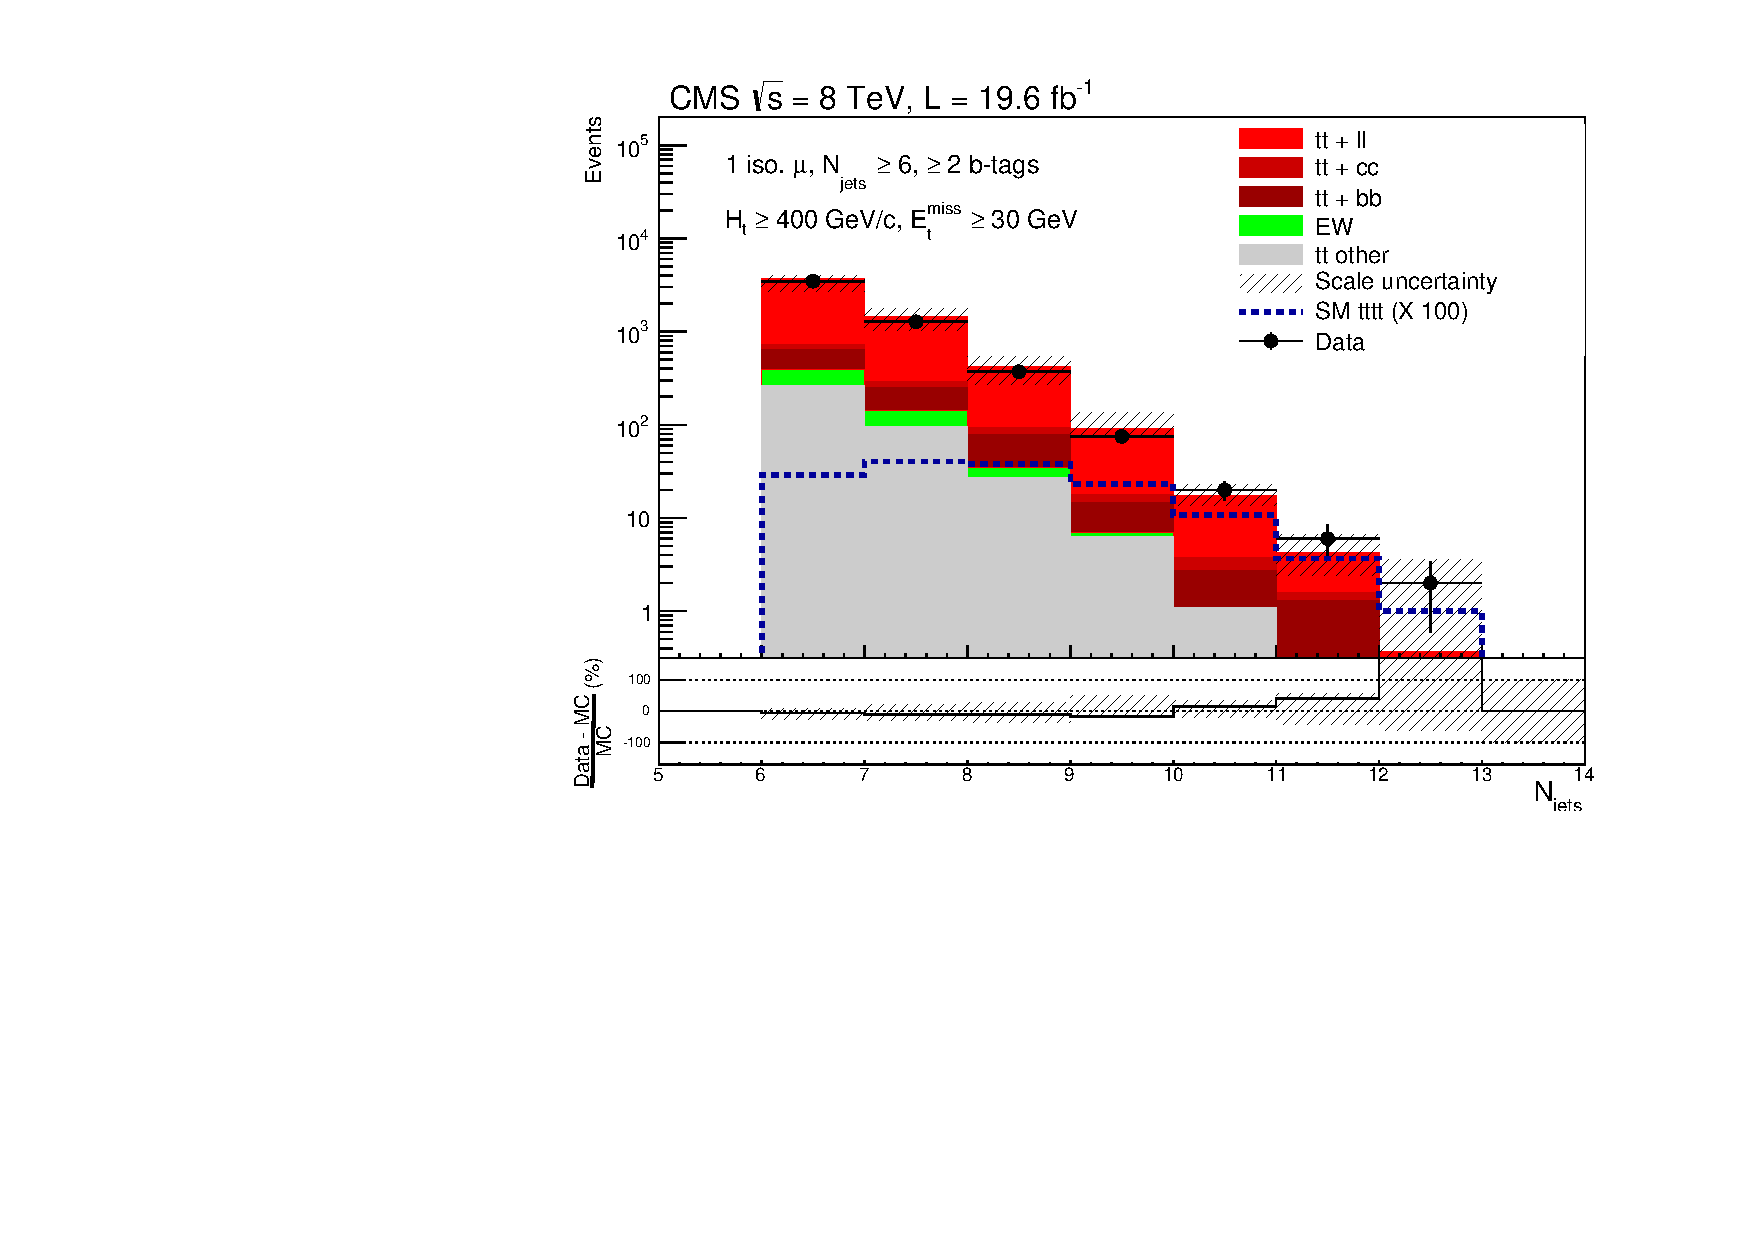
\includegraphics[width=0.49\textwidth]{images/Run1/NbOfSelectedJets_mu.pdf}
     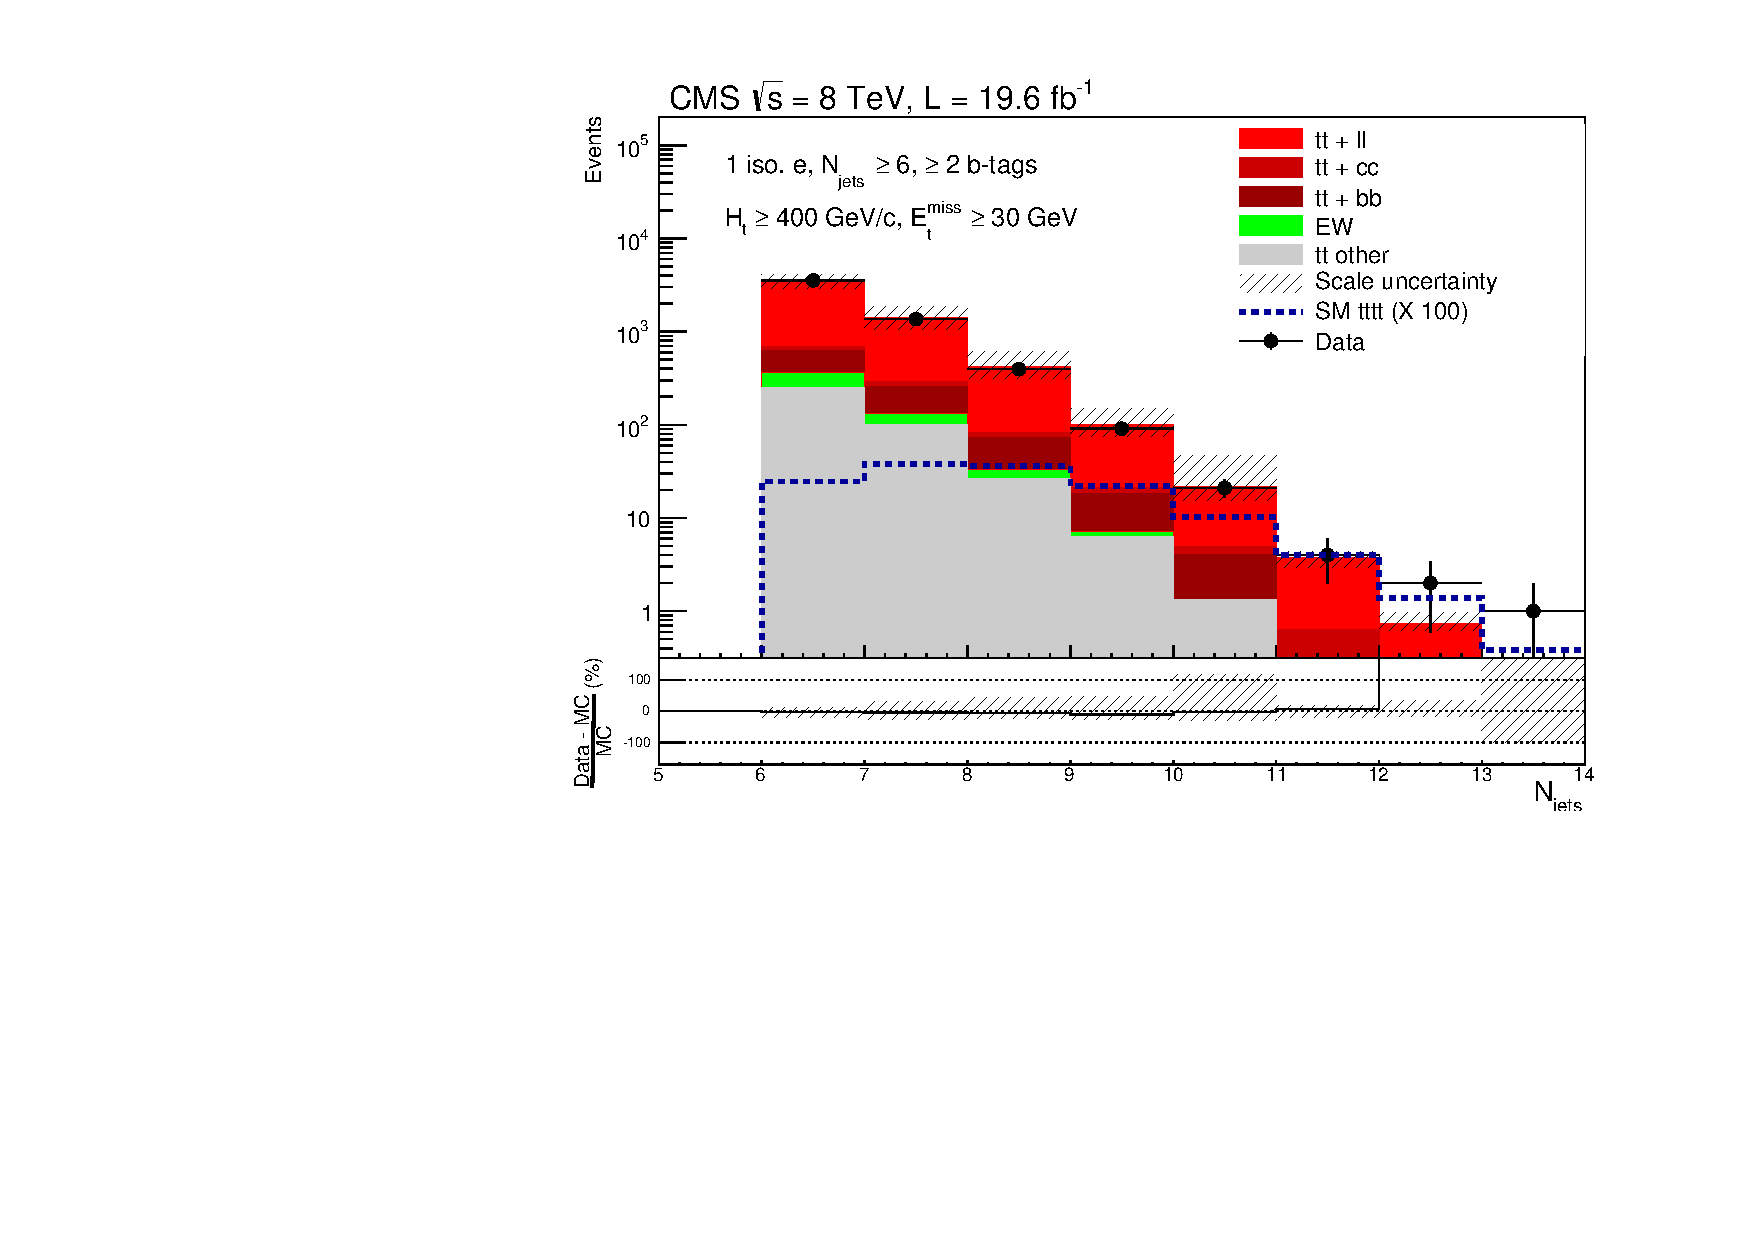
\includegraphics[width=0.49\textwidth]{images/Run1/NbOfSelectedJets_e.pdf}       
    \caption{Data-simulation comparison for \njets for $\mu$ + jets (right) and e + jets (left).}
    \label{fig:datasimnjets}
\end{figure}

\begin{figure}[ht!]
\centering
    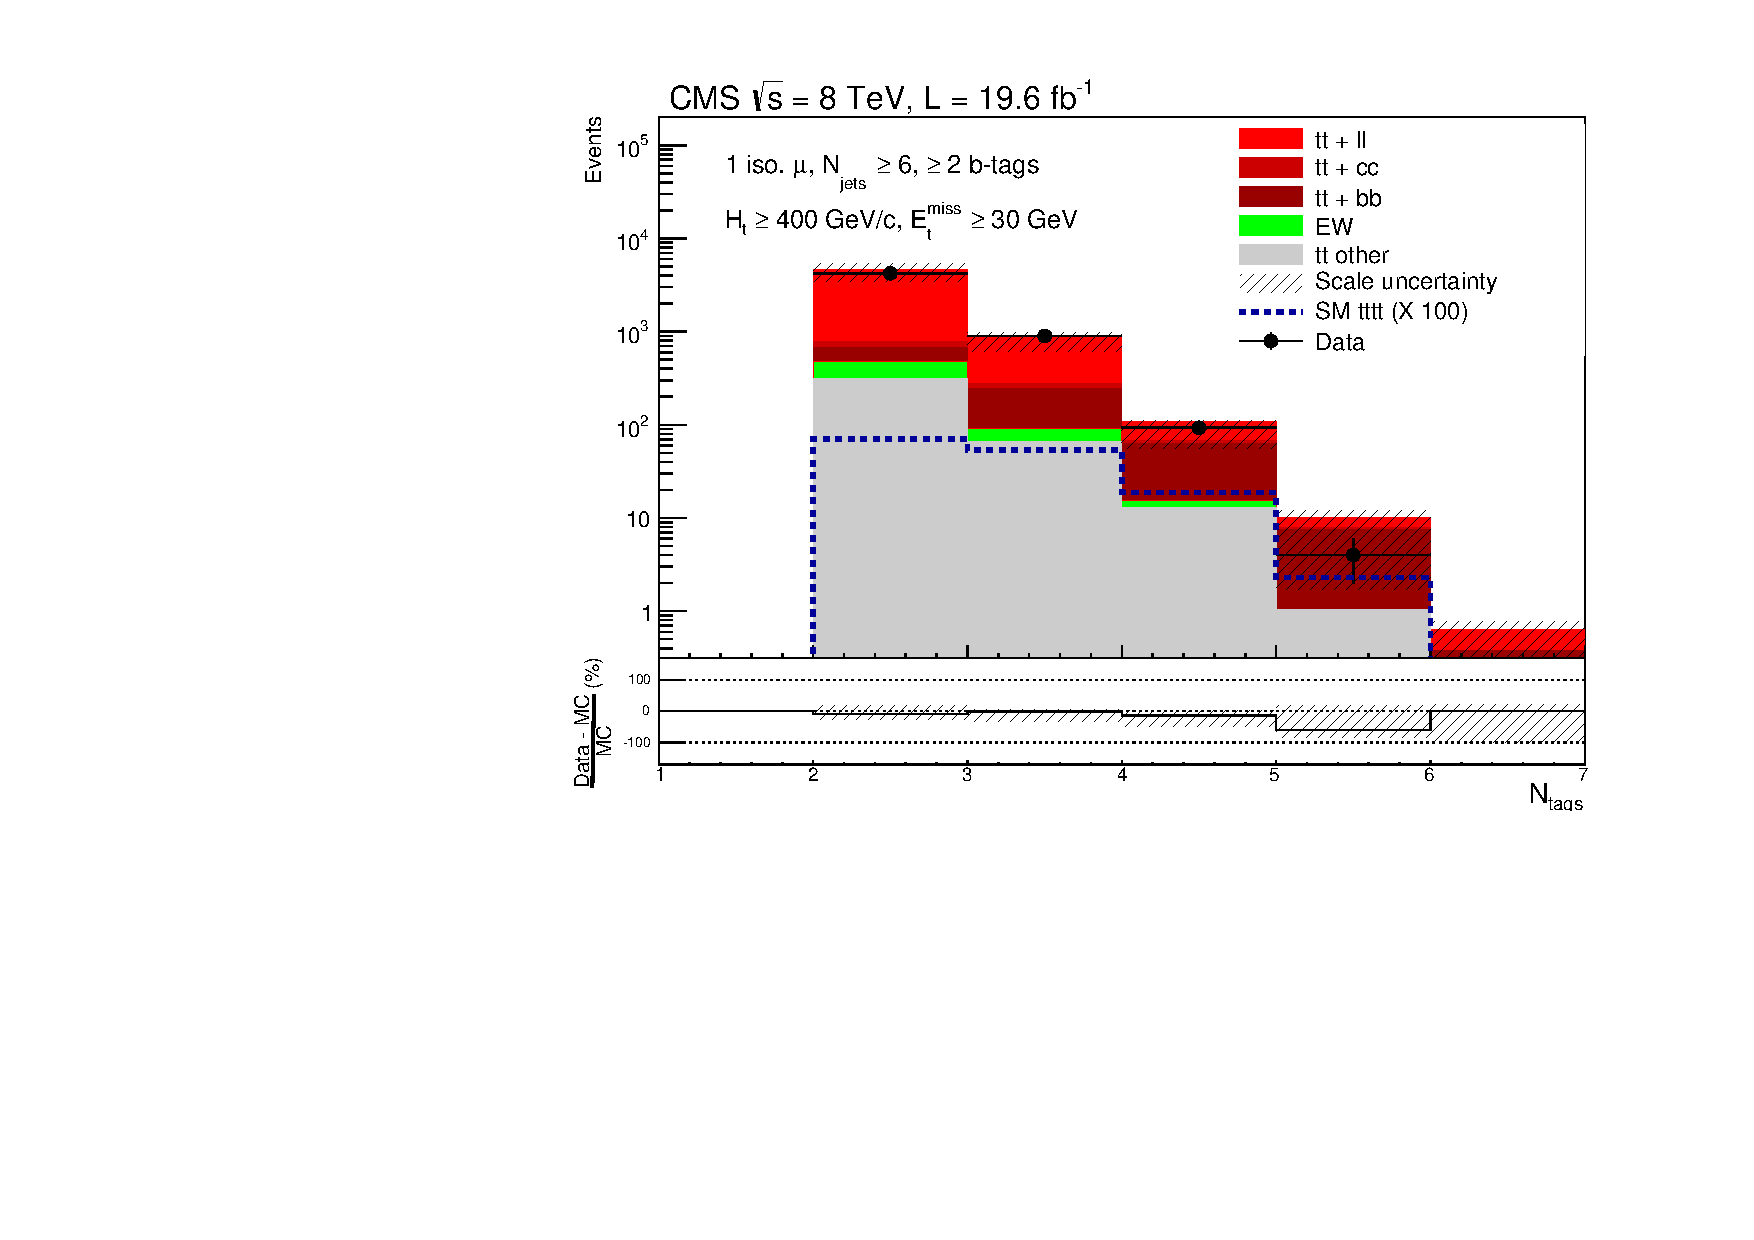
\includegraphics[width=0.49\textwidth]{images/Run1/NbOfSelectedBJets_mu.pdf}
     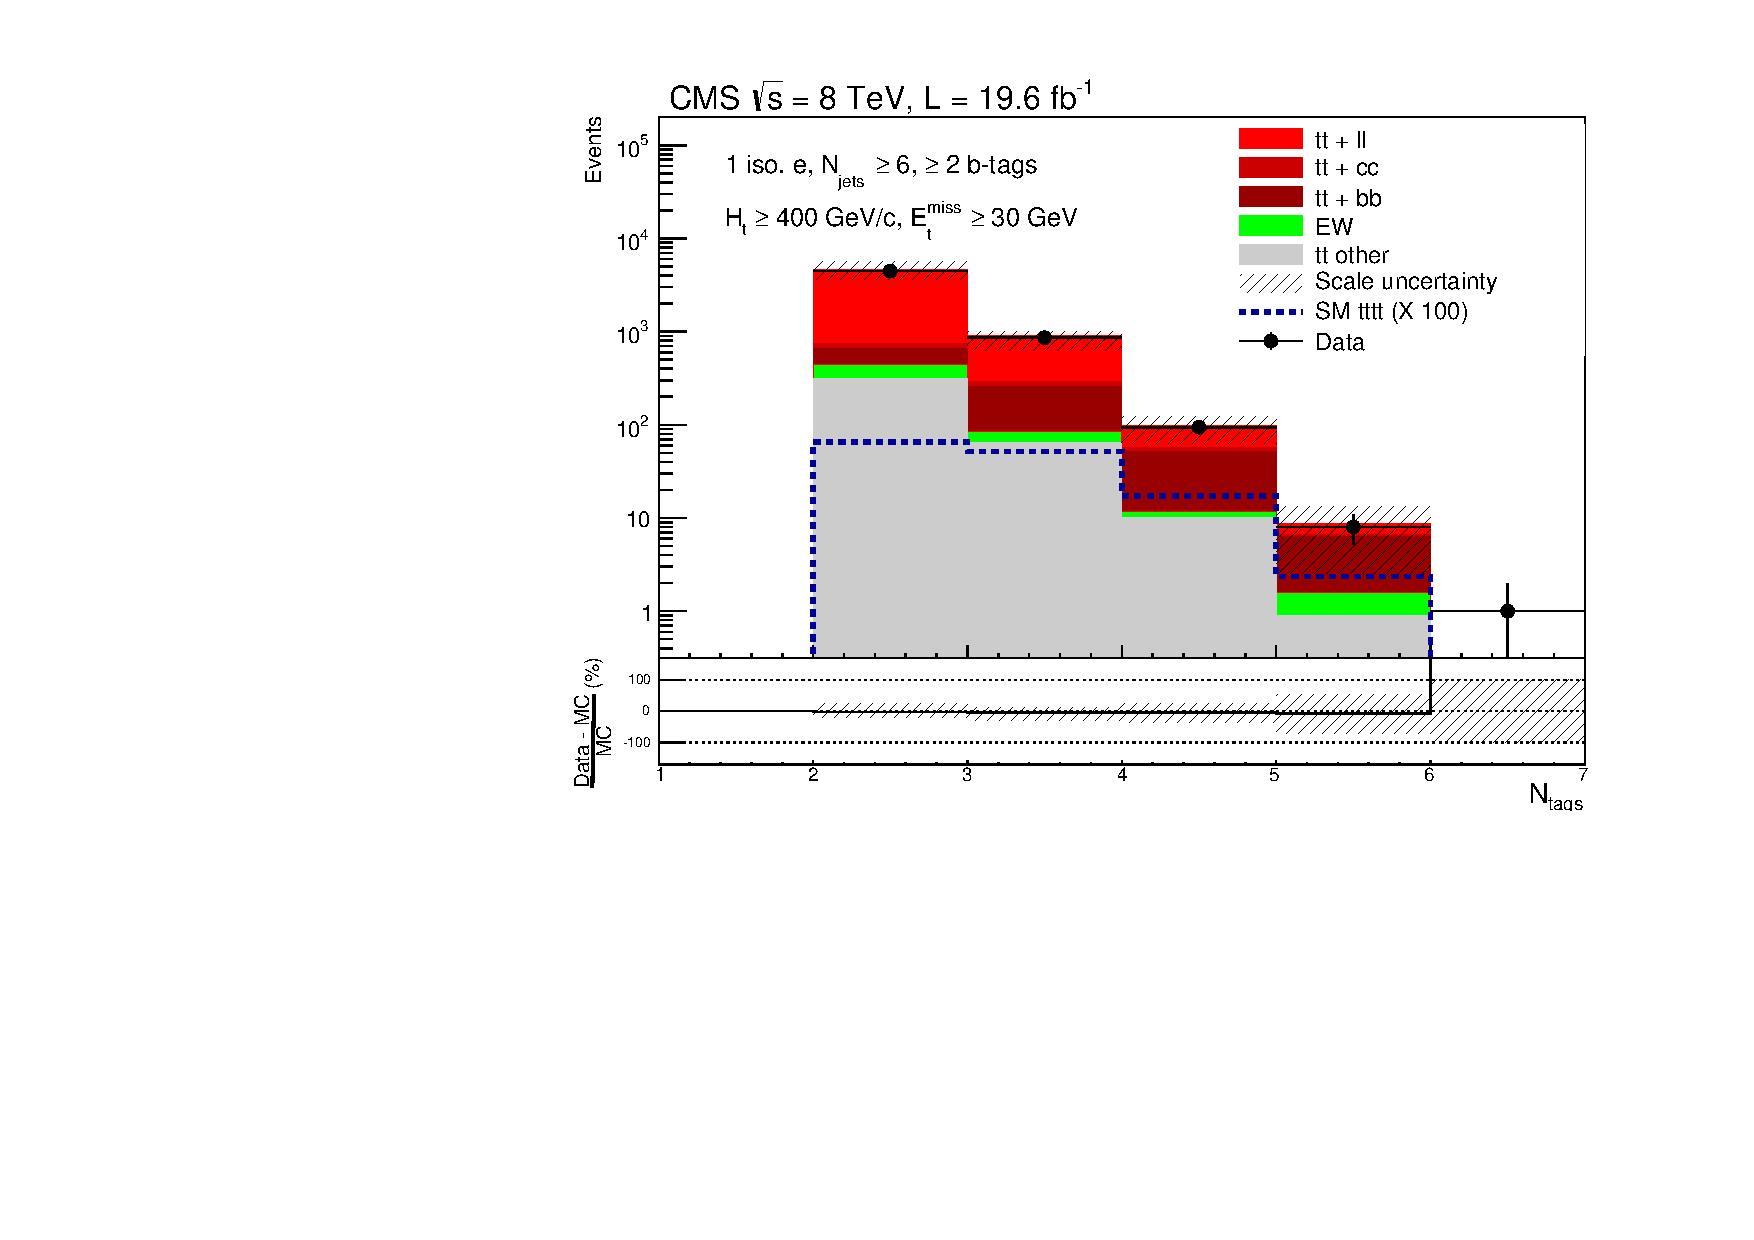
\includegraphics[width=0.49\textwidth]{images/Run1/NbOfSelectedBJets_e.pdf}        
    \caption{Data-simulation comparison for \nbtags for $\mu$ + jets (right) and e + jets (left).}
    \label{fig:datasimnbtags}
\end{figure}

\begin{figure}[ht!]
\centering
    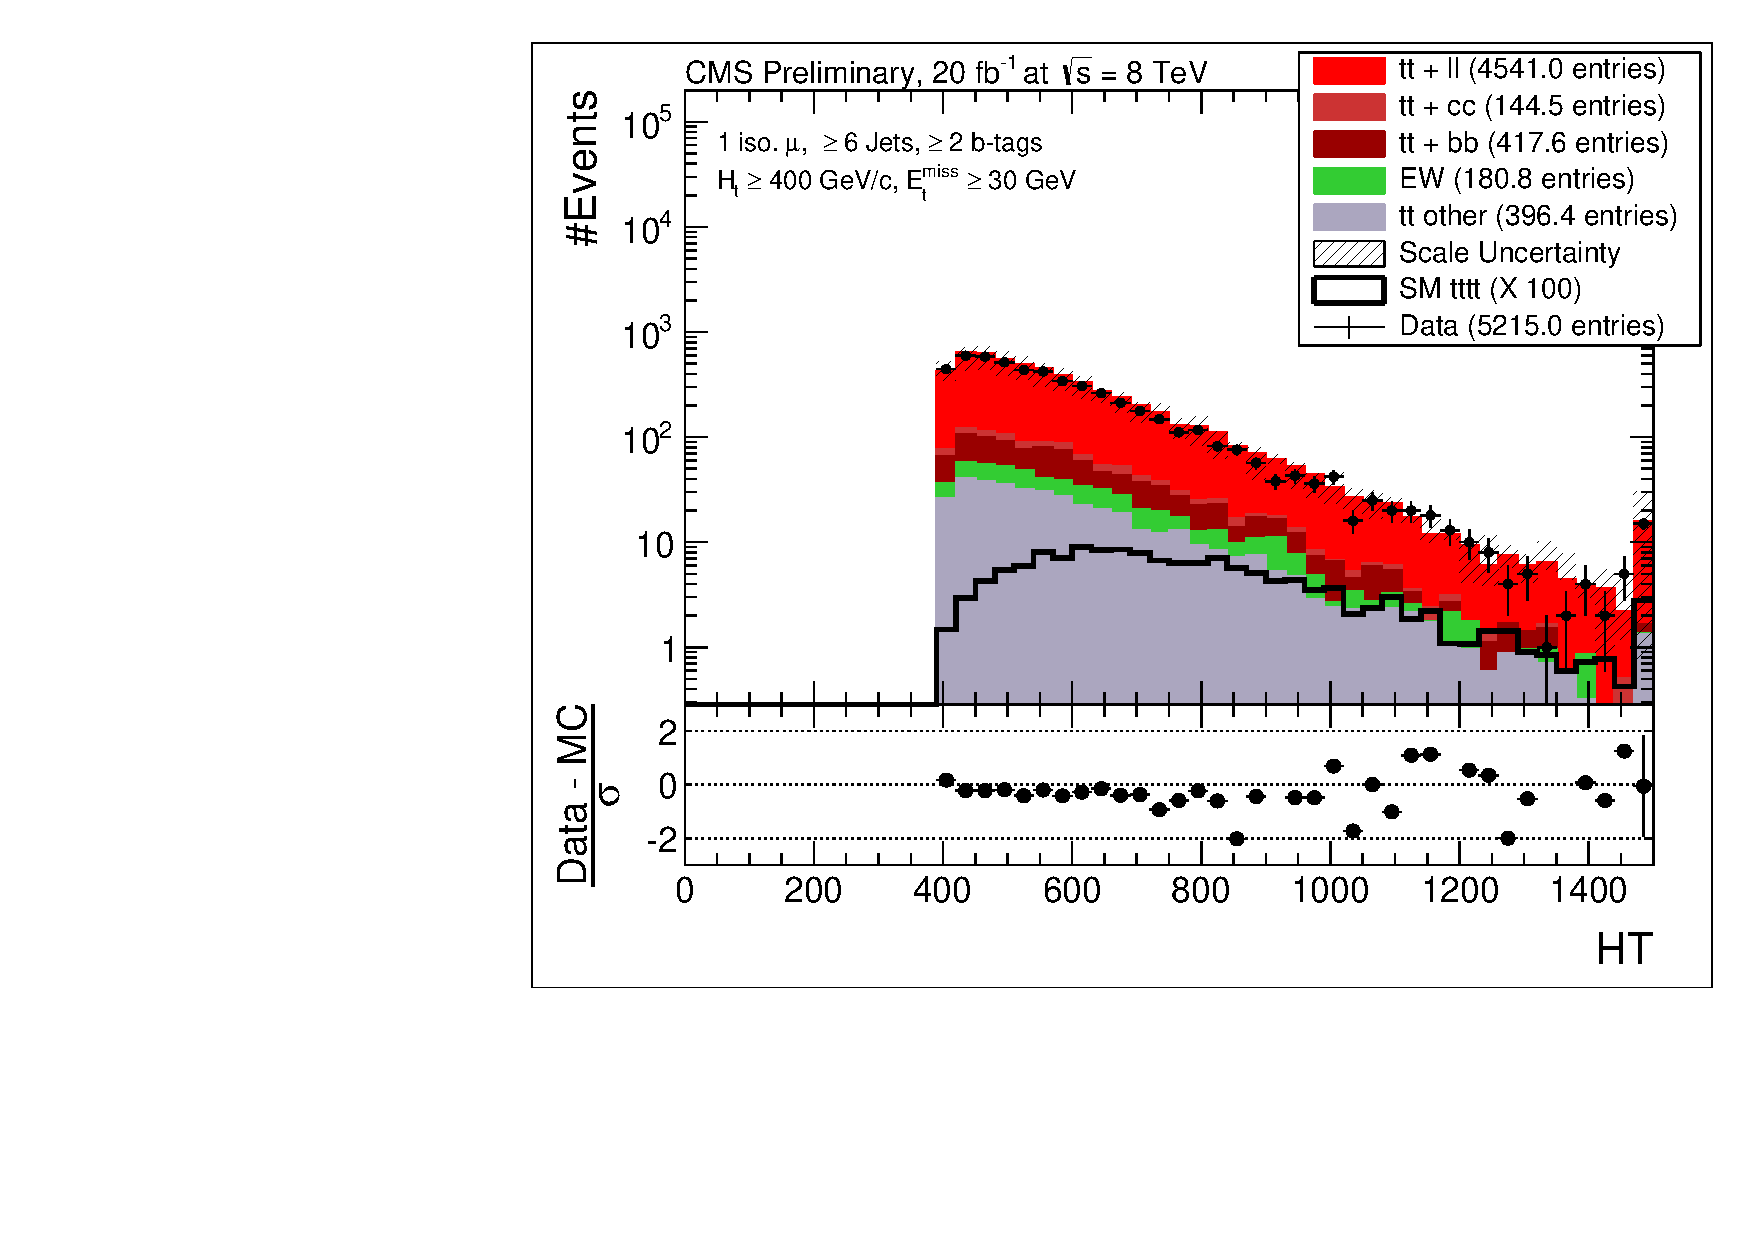
\includegraphics[width=0.49\textwidth]{images/Run1/HT_SelectedJets_StackLogY_Mu.pdf}
     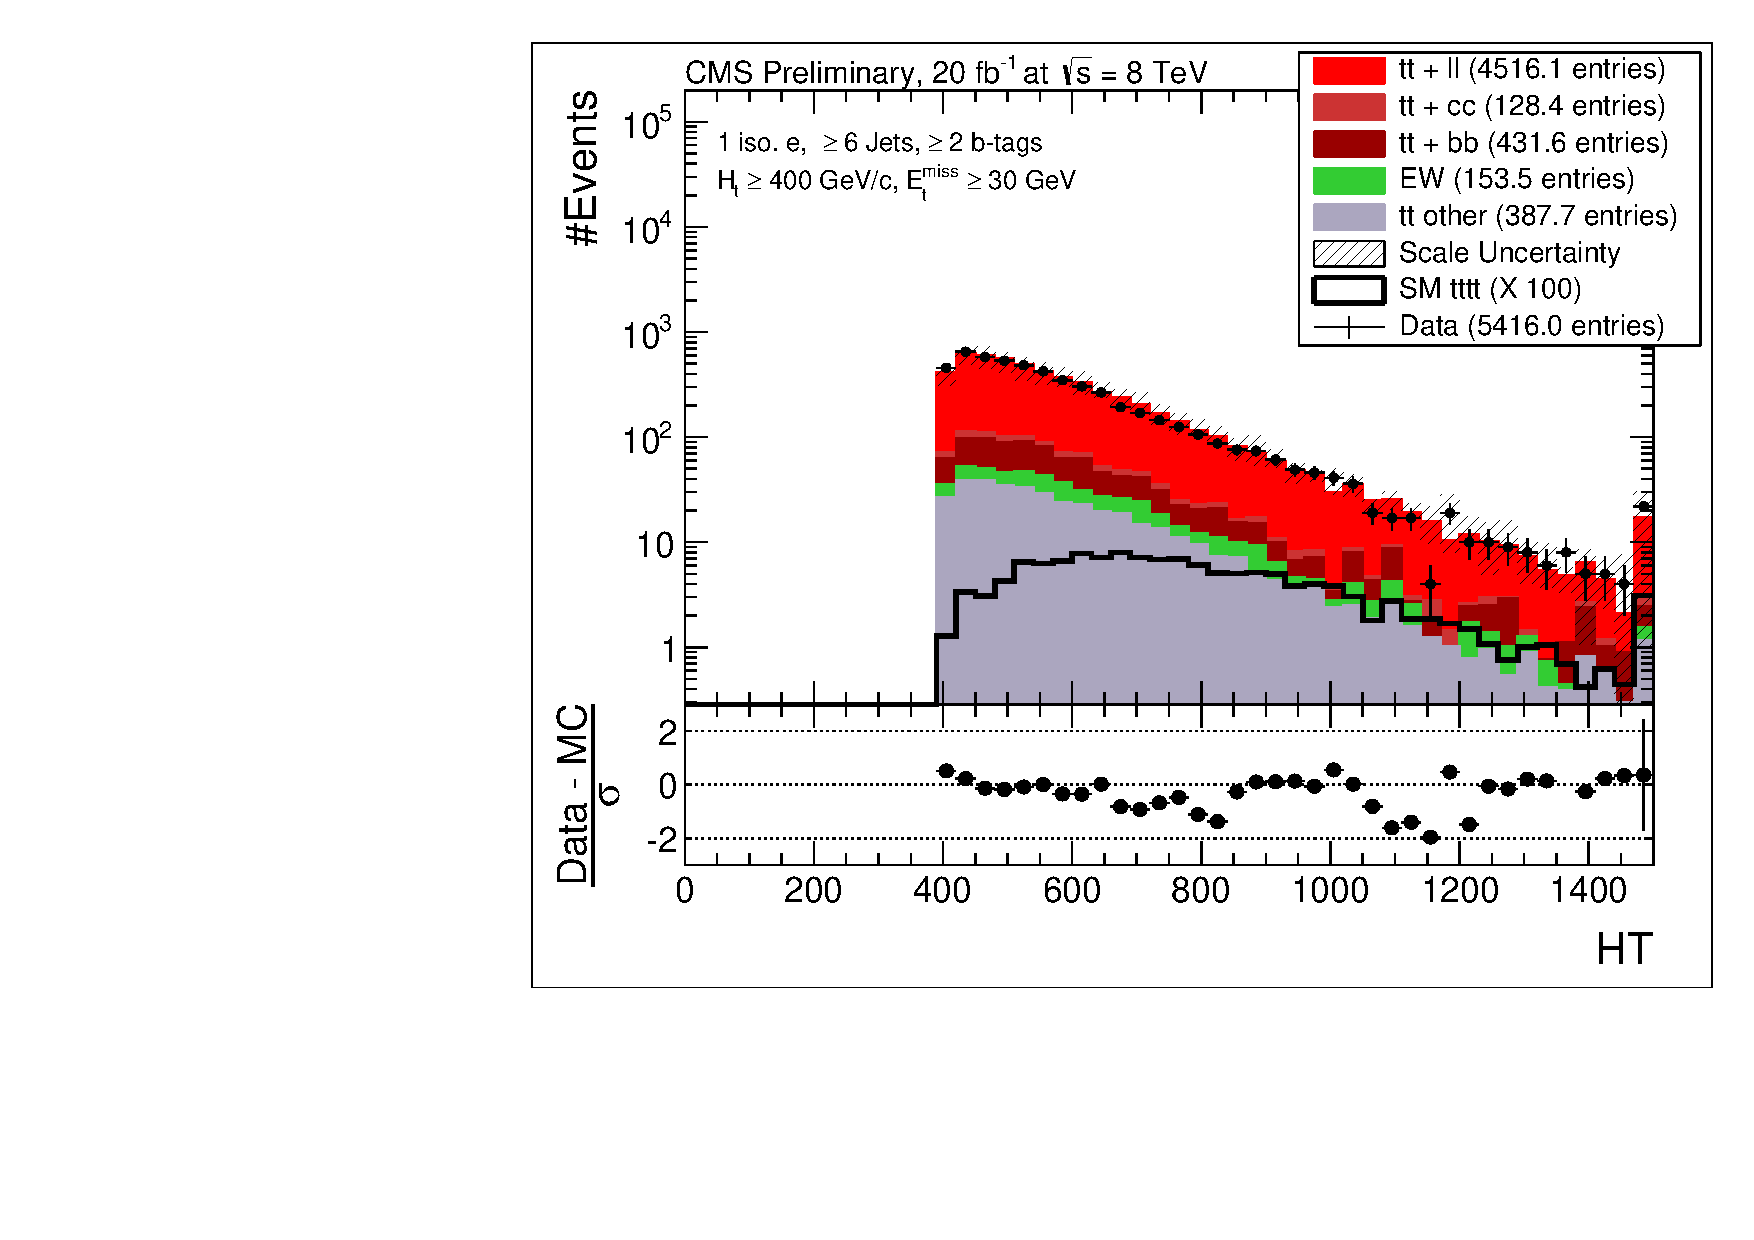
\includegraphics[width=0.49\textwidth]{images/Run1/HT_SelectedJets_StackLogY_e.pdf}          
    \caption{Data-simulation comparison for \HT for $\mu$ + jets (right) and e + jets (left). }
    \label{fig:datasimHT}
\end{figure}

\begin{figure}[ht!]
\centering
    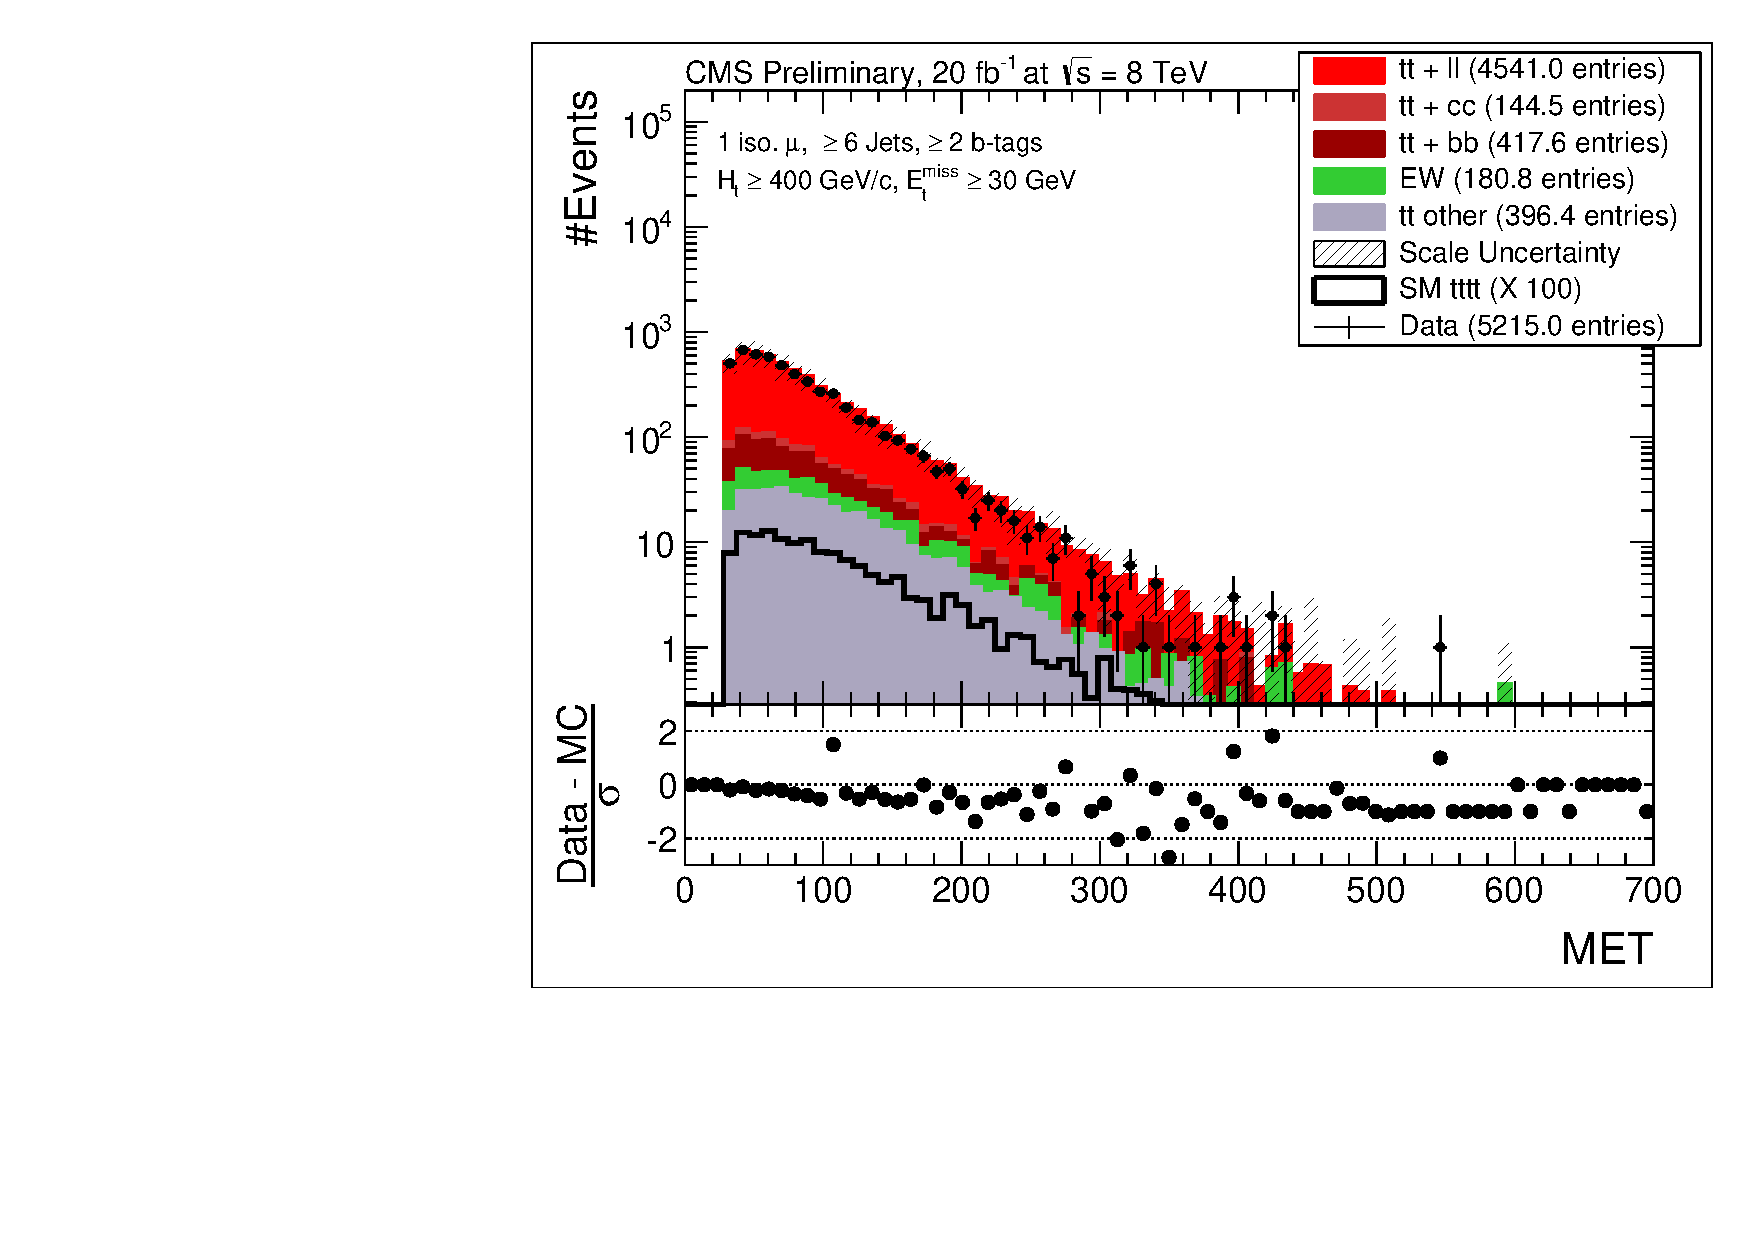
\includegraphics[width=0.49\textwidth]{images/Run1/MET_StackLogY_Mu.pdf}
     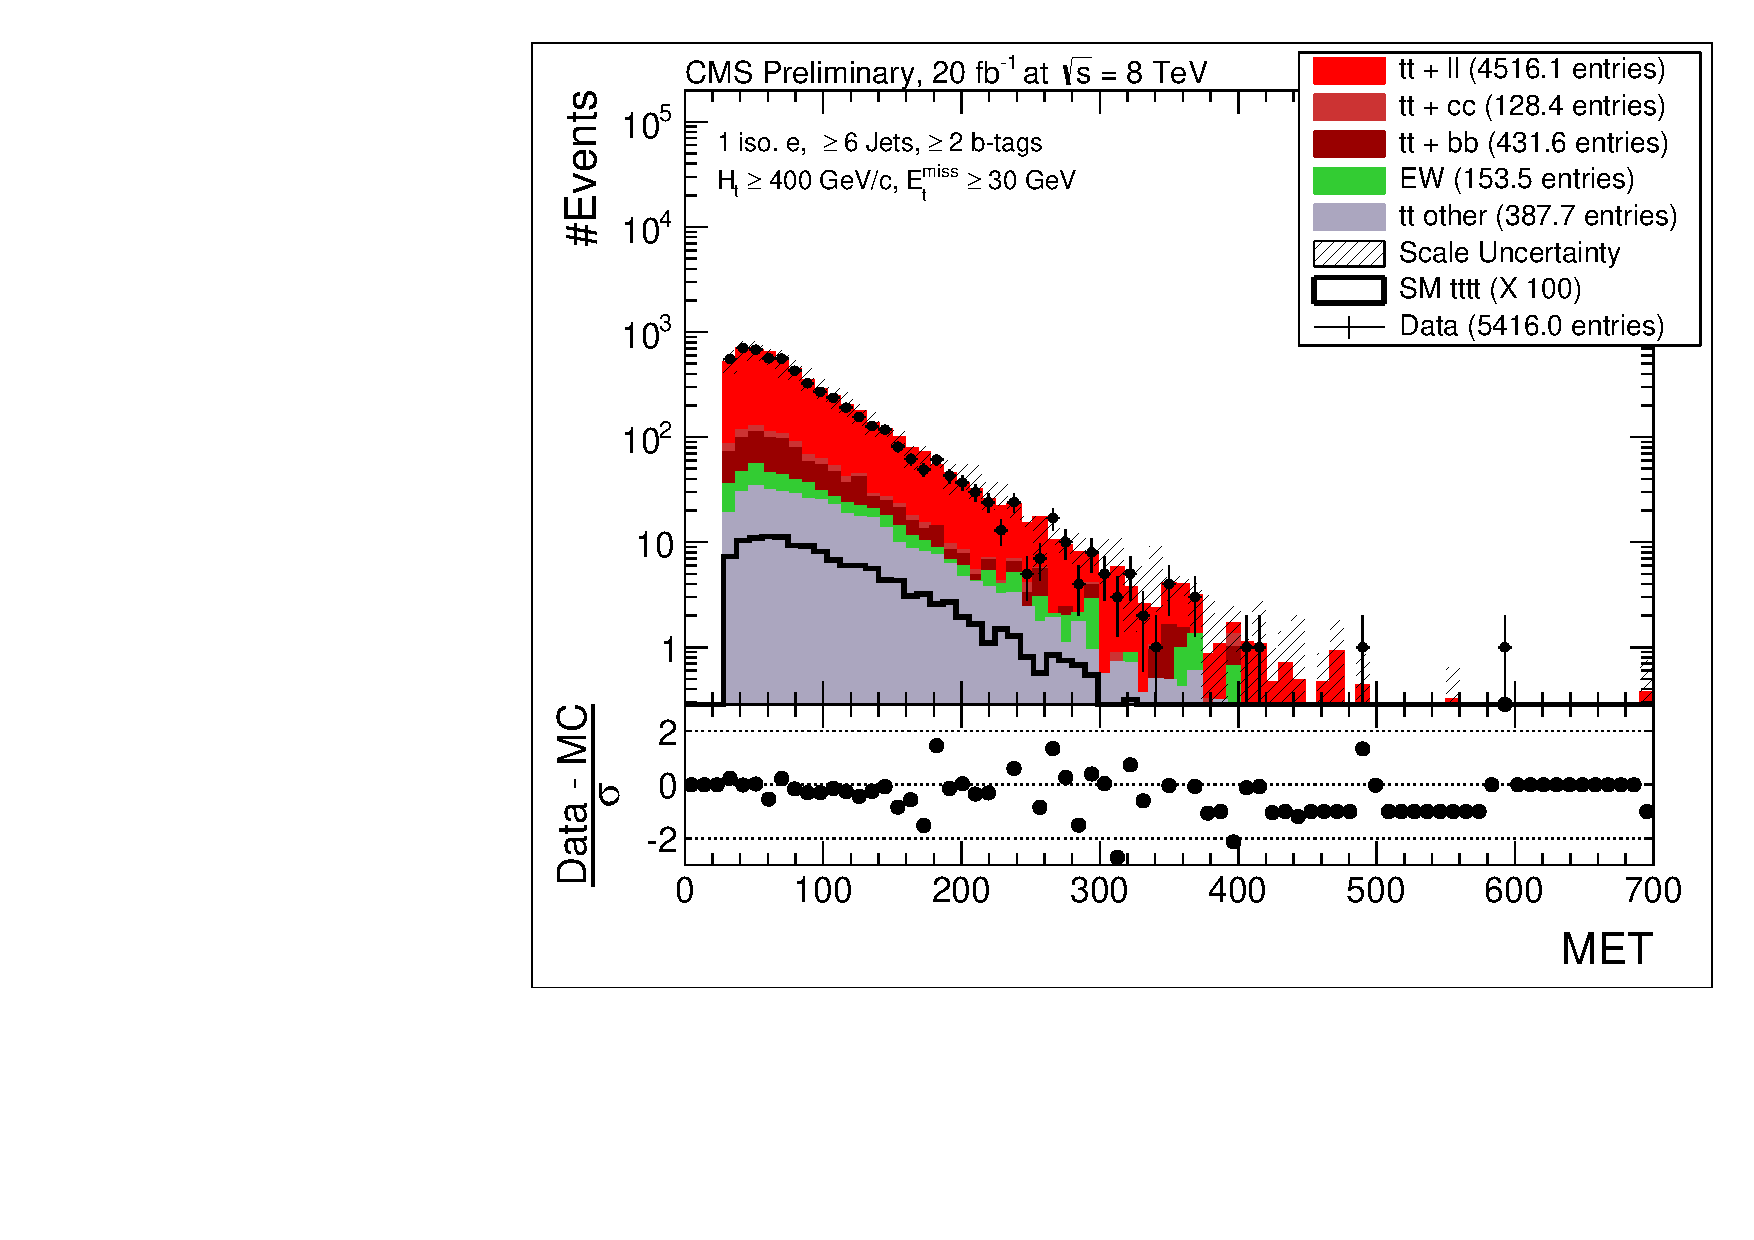
\includegraphics[width=0.49\textwidth]{images/Run1/MET_StackLogY_e.pdf}          
    \caption{Data-simulation comparison for \MET for $\mu$ + jets (right) and e + jets (left). }
    \label{fig:datasimMET}
\end{figure}



\section{Multi-jet background estimation}
\label{sec:QCDbackground}
The presence of multi-jet events within the signal region defined by the baseline selection is investigated in this section. 
%It is rare for multi-jet events to have a highly energetic undetectable particle. Therefore, the $\MET$ distributions for multi-jet events typically peak at \fxnote*{more specific?}{low values}. 
It can be seen from the MET distributions in Fig.~\ref{fig:datasimMET} that the data agrees well with the simulation at low values which suggests there are very few multi-jet events which pass the tight requirements in the baseline selection. 
%Due to this small number of events, it is not possible to use multi-jet MC to estimate this background. In this case, a data-driven method known as the \fxnote*{ref?}{ABCD method} may be used. This method proceeds by selecting two uncorrelated variables from the object or baseline selection and defining three control regions (A,B,C) and one signal region (D) in the 2-dimensional phase space of these variables. The event variable \MET and the lepton variable RelIso were selected as they are \fxnote*{uncorrelated proof??}{uncorrelated} and 
The defined regions in the uncorrelated variables of \MET and $RelIso$ are shown below. The upper bound in $RelIso$ is restricted by the minimum $RelIso$ values required by the HLT in the single muon and single electron data sets.\\

For the muon channel these are:
\begin{itemize}
\setlength\itemsep{0em}
\item A : 30 $<\MET<$ 500, 0.1 $<$ RelIso $<$ 0.15
\item B : 0 $<\MET<$ 30, 0.1 $<$ RelIso $<$ 0.15
\item C : 0 $<\MET<$ 30, 0 $<$ RelIso $<$ 0.1
\item D : 30 $<\MET<$ 500, 0 $<$ RelIso $<$ 0.1
\end{itemize}
For the \eplusjets:
\begin{itemize}
\itemsep0em
\item A : 30 $<\MET<$ 500, 0.12 $<$ RelIso $<$ 0.2
\item B : 0 $<\MET<$ 30, 0.12 $<$ RelIso $<$ 0.2
\item C : 0 $<\MET<$ 30, 0 $<$ RelIso $<$ 0.12
\item D : 30 $<\MET<$ 500, 0 $<$ RelIso $<$ 0.12
\end{itemize}

%It is assumed that the multi-jet background can be estimated from the data minus the background expectation from all of the other MC samples considered in Section~\ref{sec:datasimulation}. 
The results of the background subtraction from data and the defined ABCD regions are shown in Fig.~\ref{fig:QCDplots}.
The number of multi-jet events, N$_{\textrm{multi-jet}}$, in each of the control regions are used to predict the number of multi-jet events in region D using Eq.~\ref{N-multi-jet}, the results of which are shown in Table~\ref{tab:multijet}.

\begin{figure}[!ht]
    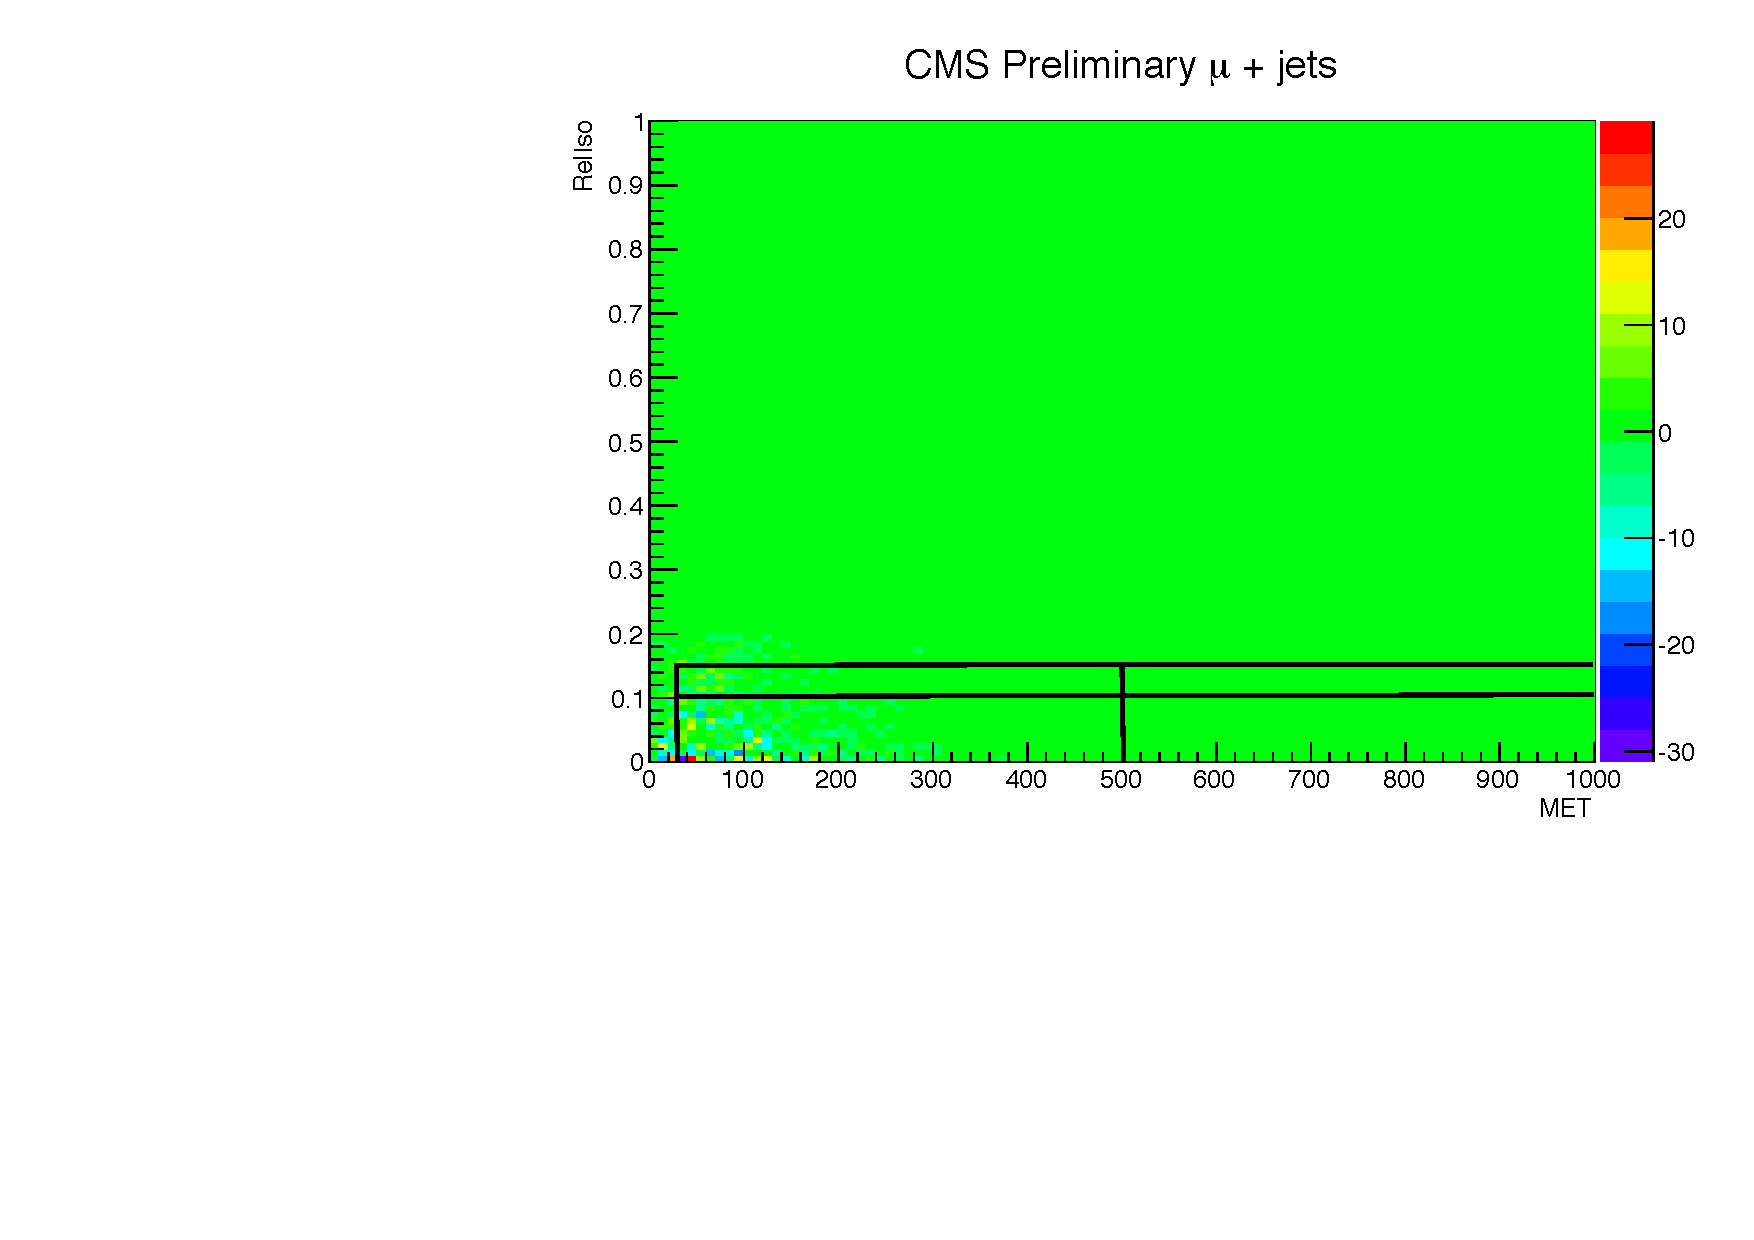
\includegraphics[width=0.49\textwidth]{images/Run1/Data_Minus_MC_Mu_Lines.pdf}
    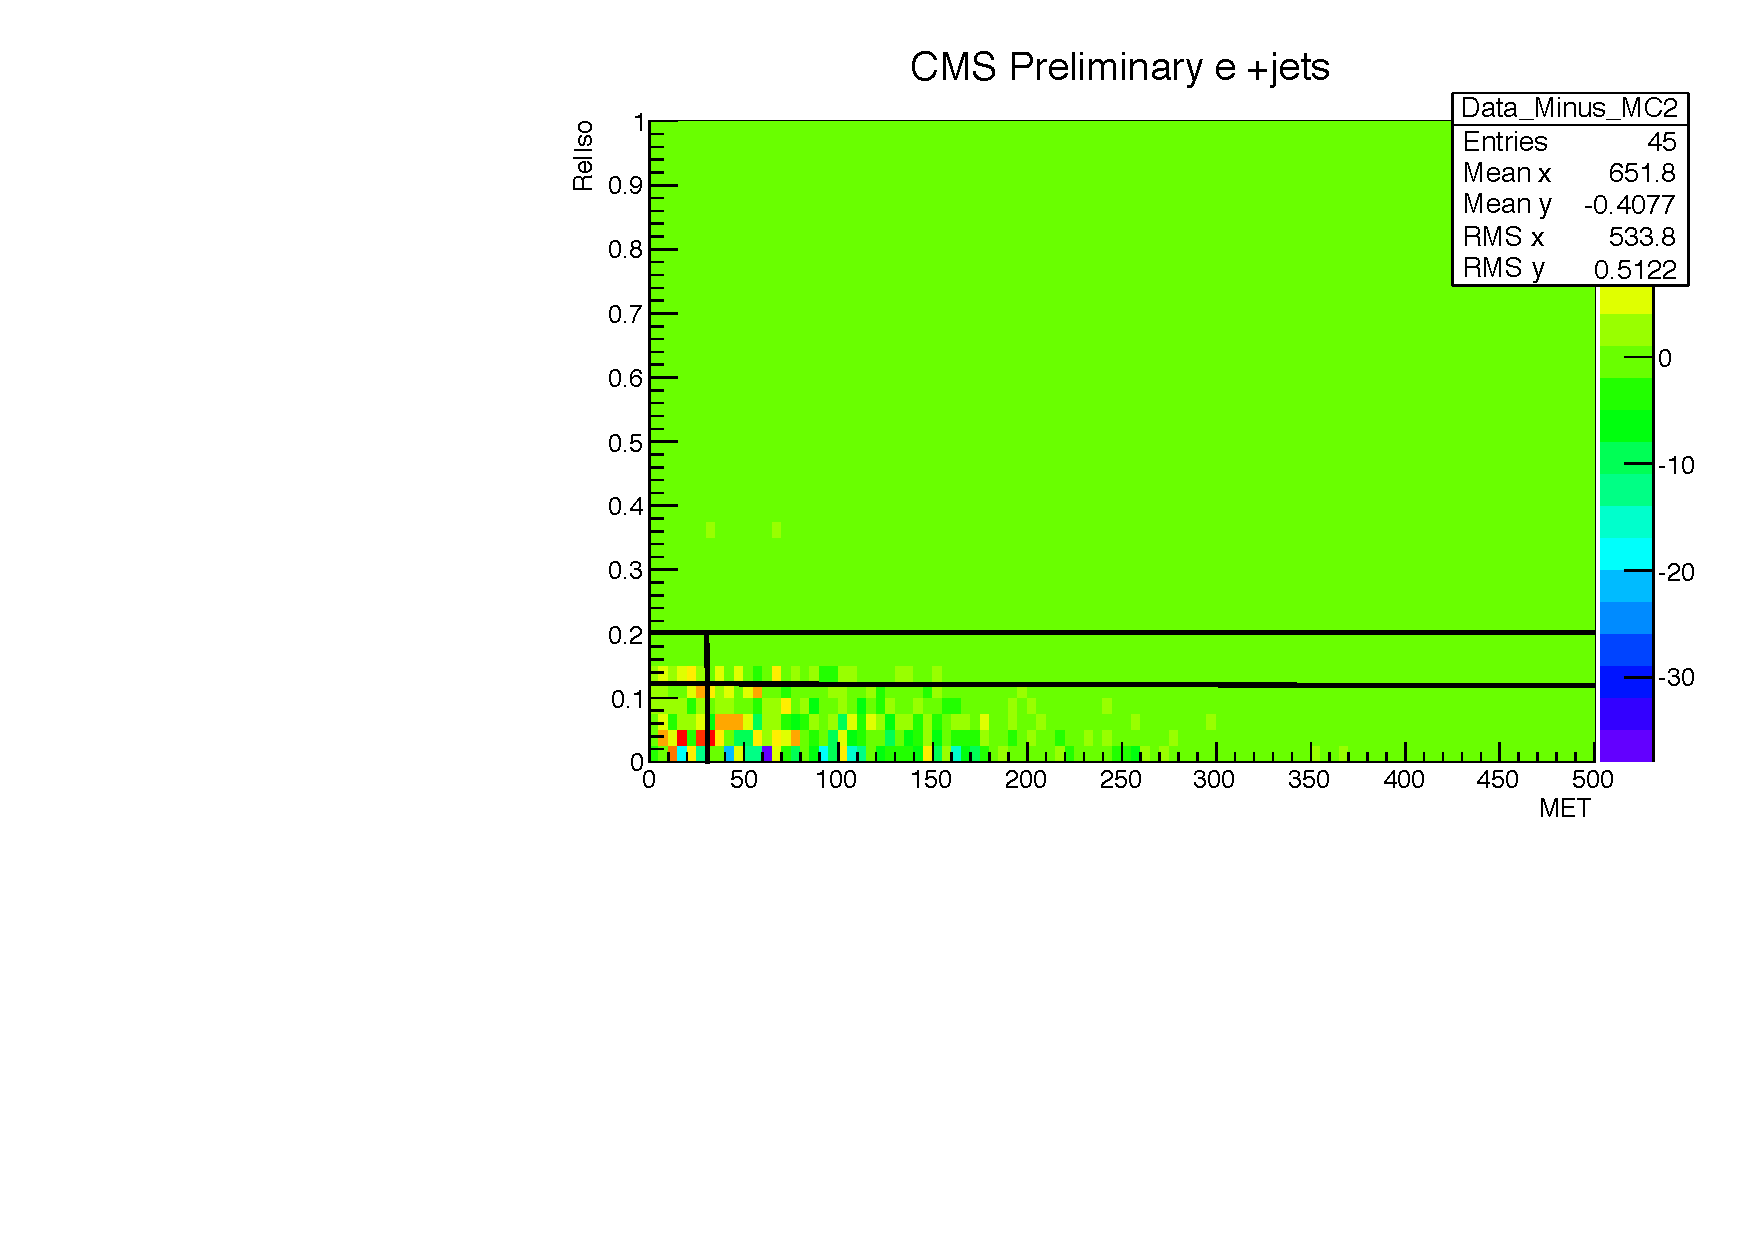
\includegraphics[width=0.49\textwidth]{images/Run1/Data_Minus_MC_El_Lines.pdf}
    \caption{Data minus MC background for MET vs lepton iso for $\mu$ + jets (right) and e + jets (left).}
    \label{fig:QCDplots}
\end{figure}


\begin{equation}
\frac{\textrm{N}^{\textrm{B}}_{\textrm{multi-jet}}}{\textrm{N}^{\textrm{A}}_{\textrm{multi-jet}}} = \frac{\textrm{N}^{\textrm{C}}_{\textrm{multi-jet}}}{\textrm{N}^{\textrm{D}}_{\textrm{multi-jet}}}
\label{N-multi-jet}
\end{equation}

\begin{table}[ht!]
\caption{Multi-jet estimation}
\centering
\begin{tabular}{|c |c |c |c |c |}
 \hline 
 Channel & N$^{\textrm{A}}_{\textrm{multi-jet}}$  & N$^{\textrm{B}}_{\textrm{multi-jet}}$ & N$^{\textrm{C}}_{\textrm{multi-jet}}$ & Prediction for N$^{\textrm{D}}_{\textrm{multi-jet}}$  \\
  \hline
$\mu$ + jets & 19.1 & 16.1 & -16.8 & -20  \\
 \hline
$e$ + jets & 36.8  & 50.8 & 62.7 &45.5  \\
\hline
\end{tabular}
\label{tab:multijet}
\end{table}

As the number of \ttbar events in simulation has fluctuated to be greater than the data in region C in the muon channel, the prediction for the signal region D is negative. As this prediction is unphysical, the number of events is estimated to be zero in the muon channel. In the electron, 45.5 multi-jet events are predicted which is considered negligible at $<1\%$ of the massive \ttbar background. Hence, the multi-jet background is not considered further.
% \fxnote{scale up scale down...200\% uncertainty?}

\section{Discriminating between signal and background}
\label{sec:discriminating}
As seen from the cut flow in section~\ref{cutflow}, the dominant background process after the baseline selection is \ttbar production, which is three orders of magnitude greater than the \tttt signal process in the signal region.
In this section, details of the hadronic top quark reconstruction described in section~\ref{sec:topreco} and the variables that can be defined as a result of this MVA will be discussed as well as the variables which are used in the event-level BDT

 % This motivates the search for variables which can discriminate between these two processes.
  There are three main features which can be used to discriminate; the number of top quarks which can be reconstructed in the event, the number of b-jets found in each event, and event activity such as \HT.

\subsection{Hadronic top quark content}
\label{sec:topContent}
% In the single lepton channel for \tttt production, there are three top quarks where the W boson decays hadronically, these will be referred to as hadronic top quarks. For the main background of \ttbar there is only one hadronic top quark. Additional jets in \ttbar come from \fxnote*{assume previously defined}{ISR or FSR} in order to satisfy the requirements of the baseline selection. Therefore, it should only be possible to reconstruct more than one top quark from three jets originating from it's hadronic decay in \tttt but not in \ttbar. However, 

The \antikt algorithm can only distinguish separate jets if they have \DR$>0.5$ between them, hence it may not always be possible to reconstruct all hadronic top quarks. To ascertain whether this might be a powerful technique for separating \tttt and \ttbar or not, 1000 \tttt and 1000 \ttbar events were analysed where there was one muon with \PT $>$ 26 GeV and exactly 6 jets with \PT $>$ 30 and $\lvert \eta \rvert<$ 2.5. Hadronic top quarks are considered reconstructible at parton level if they decayed into jets with \DR  $>$  0.5. The number of reconstructible hadronic top quarks for \tttt and \ttbar are shown in Fig.~\ref{fig:ReconHadTops}.

\begin{figure}[!ht]
\centering

    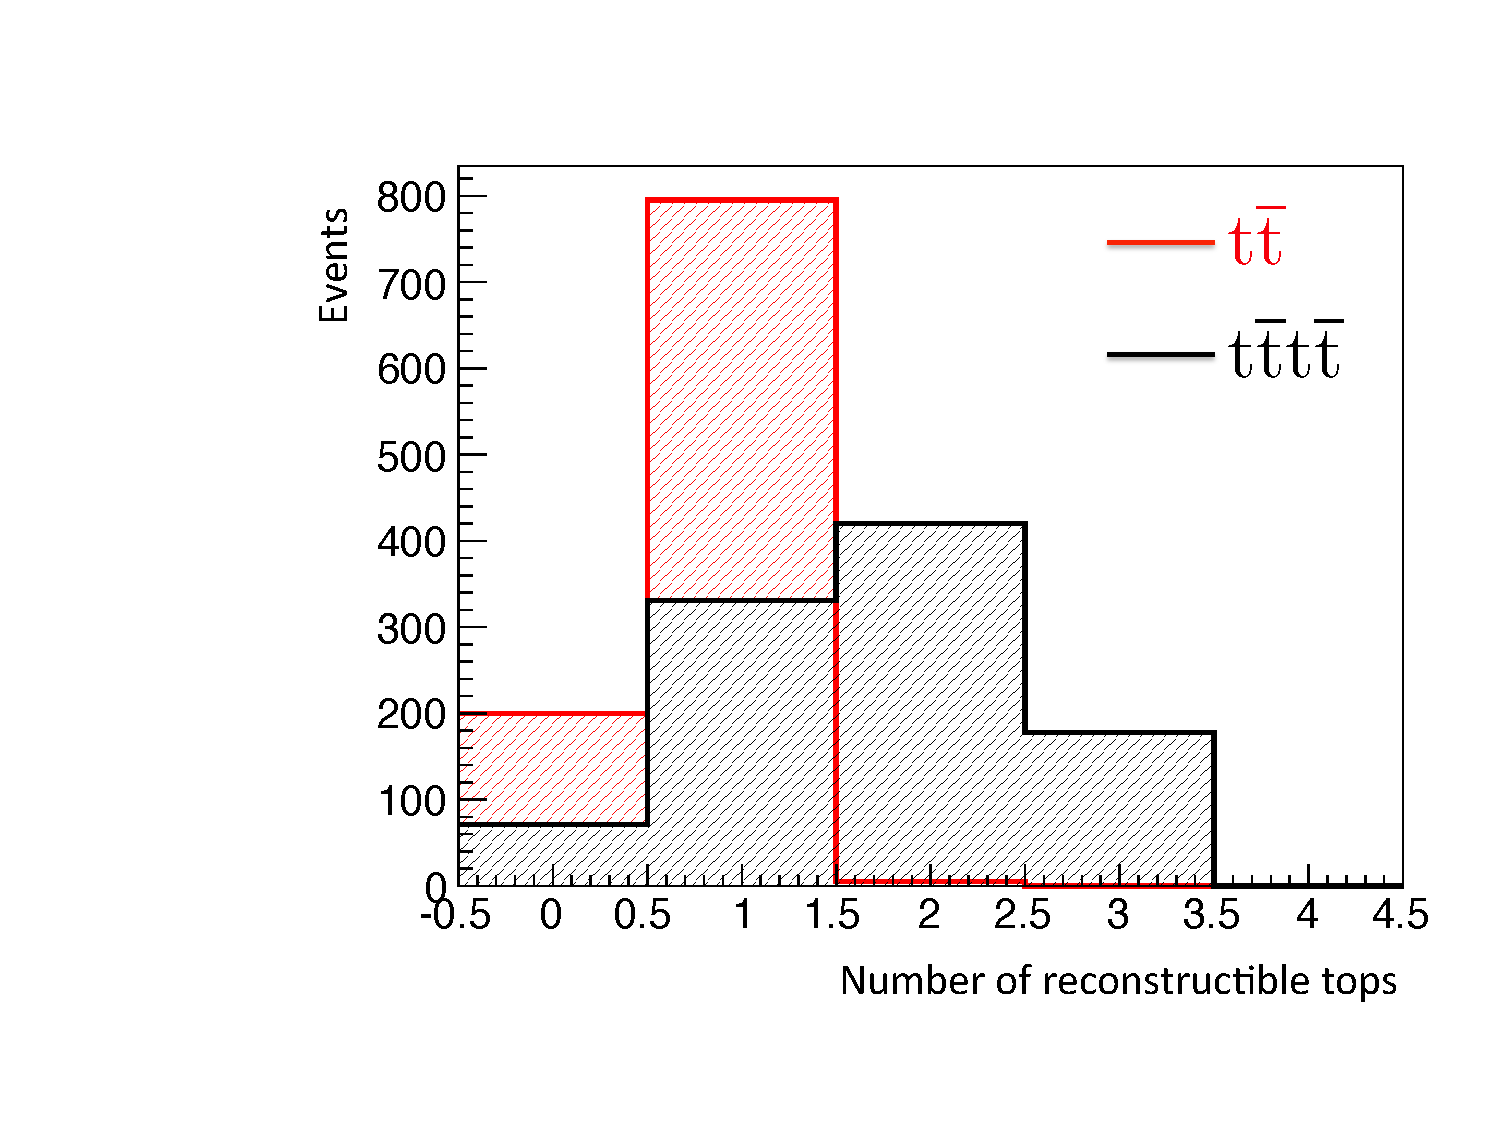
\includegraphics[width=0.6\textwidth]{images/Run1/HadRecoTops.pdf}
    \caption{The number of reconstructible hadronic top quarks in \tttt and \ttbar}
    \label{fig:ReconHadTops}
\end{figure}

For \tttt production at parton level it is possible to reconstruct more than one hadronic top quark $\approx$ 63 $\%$ of the time compared to a negligible number of times in \ttbar, as is evident in the Fig.~\ref{fig:ReconHadTops}. Hence, using the number of hadronic tops can be assumed to be a powerful variable worth investigating. 
% One obstacle to this is the large number of ways in which the jets can be combined in events with \njets $\geq 6$.\fxnote{more on combinatorics? -> but James' work} 

% This motivates the use of multi-variate analysis to distinguish between good tri-jet combinations and bad tri-jet combinations, where a tri-jet refers to any given combination of three jets. Figure~\ref{fig:TopBDTinput} shows the minimal number of discriminating variables which are used including:\\
% \textbf{Tri-jet invariant mass} - Good tri-jet combinations should have an invariant mass distribution which peaks around the top mass.\\
% \textbf{Di-jet invariant mass} - The di-jet combination is formed from the two jets with the smallest \DR separation. The invariant mass distribution should peak around the W mass.\\
% \textbf{\ptrat} - This is the ratio of the vectorial \pt to the scalar sum of the \pt of the jets in the tri-jet combination.\\
% \textbf{\DPTW} - This is the \Dphi separation between the tri-jet and di-jet system.\\
% \textbf{\DPTb} - This is the \Dphi separation between the tri-jet and remaining jet not included in the di-jet system.\\
% \textbf{\CSVj} - For the jet not used in the di-jet system, the CSV b-tagging discriminator value is used.\\

The variables used in the hadronic top quark reconstruction BDT are shown in Fig.~\ref{fig:TopBDTinput} where it can be seen that the tri-jet and dijet invariant masses provide the most powerful separation. This visualisation can help in finding discriminating variables but it should be considered that the shapes of these distributions will changes as the events progress through the BDT where certain events will become more heavily weighted. For instance the $CSV_{j}$ variable appears to not have much separation power initially but the distribution may look quite different in certain areas of phase space or after boosting weights have been applied and the inclusion of this variable improved the overall separation of the BDT output discriminator.

\begin{figure}[ht!]
\centering
    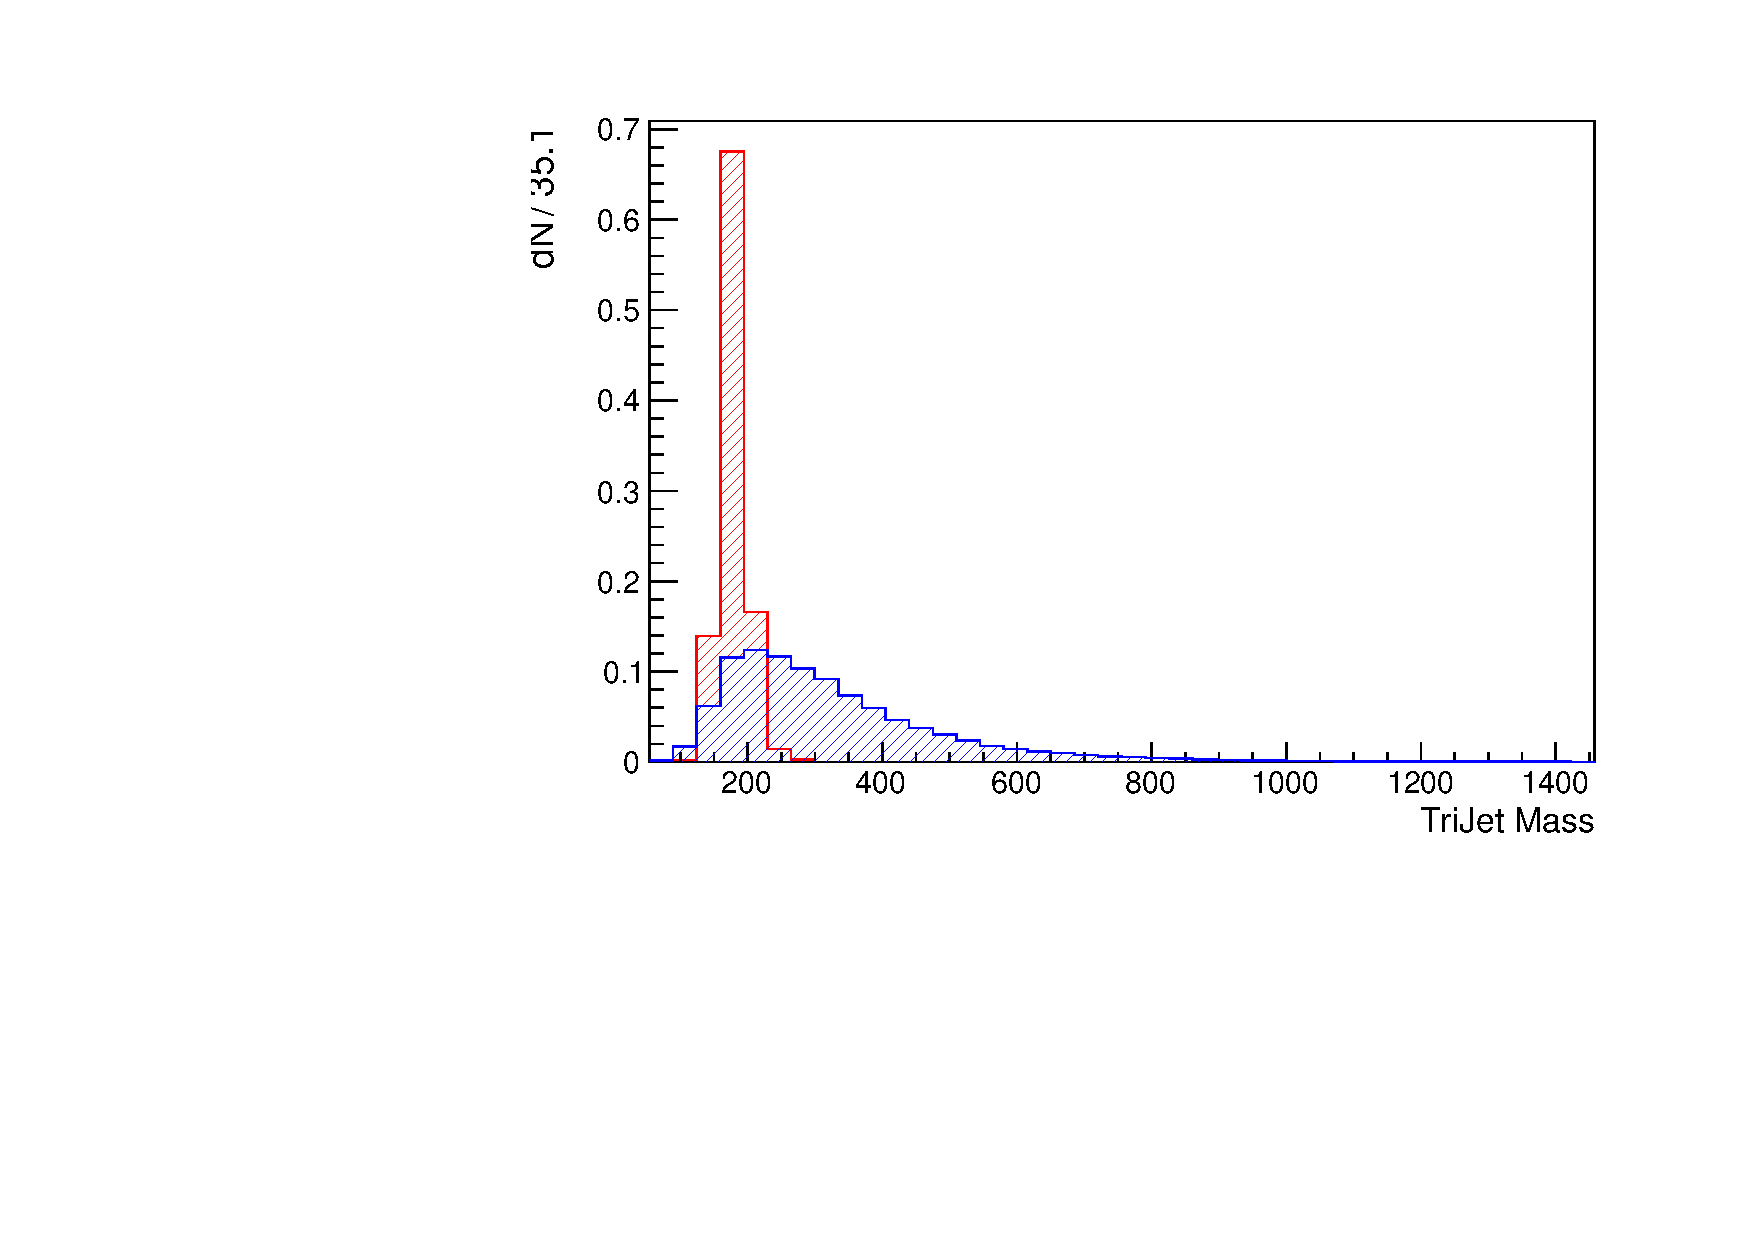
\includegraphics[width=0.49\textwidth]{images/Run1/TriJetMass.pdf}
     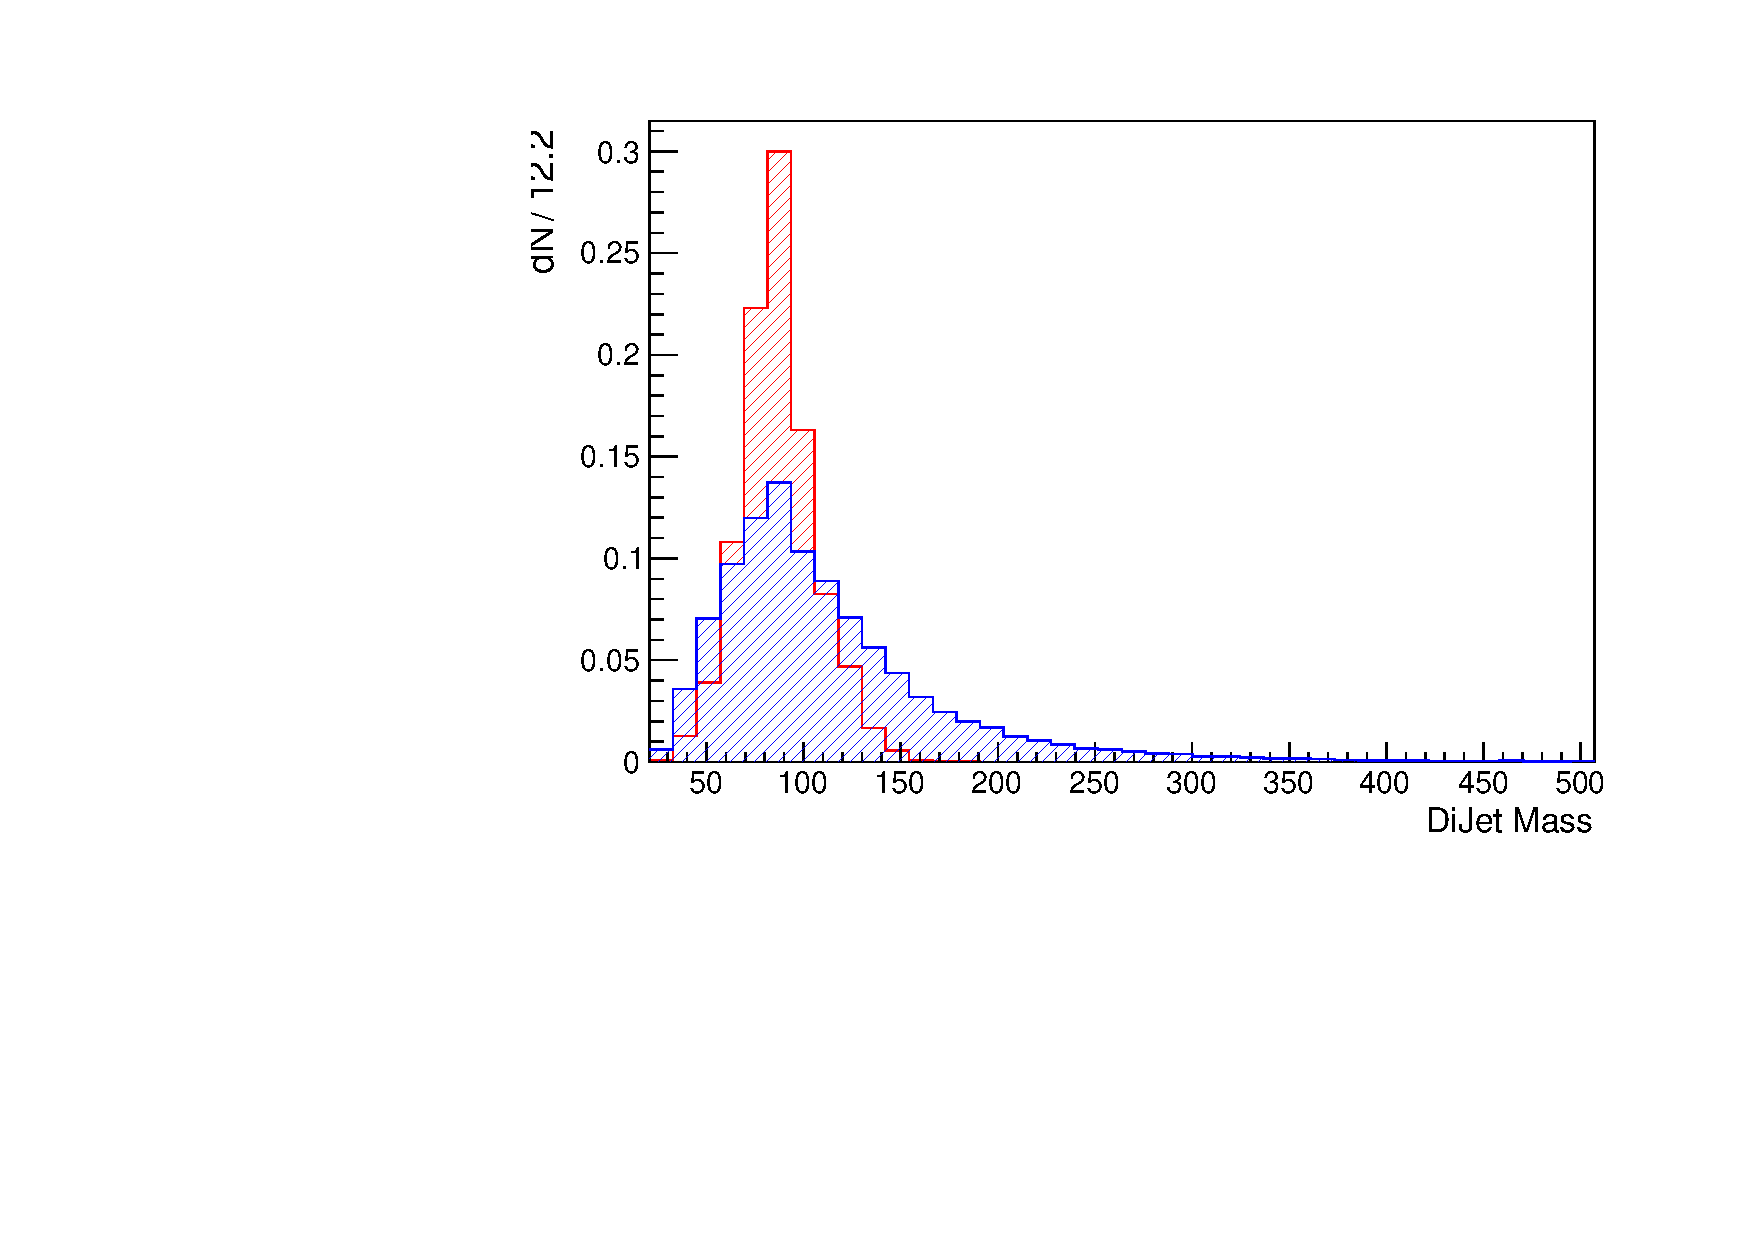
\includegraphics[width=0.49\textwidth]{images/Run1/HadWMass.pdf}
    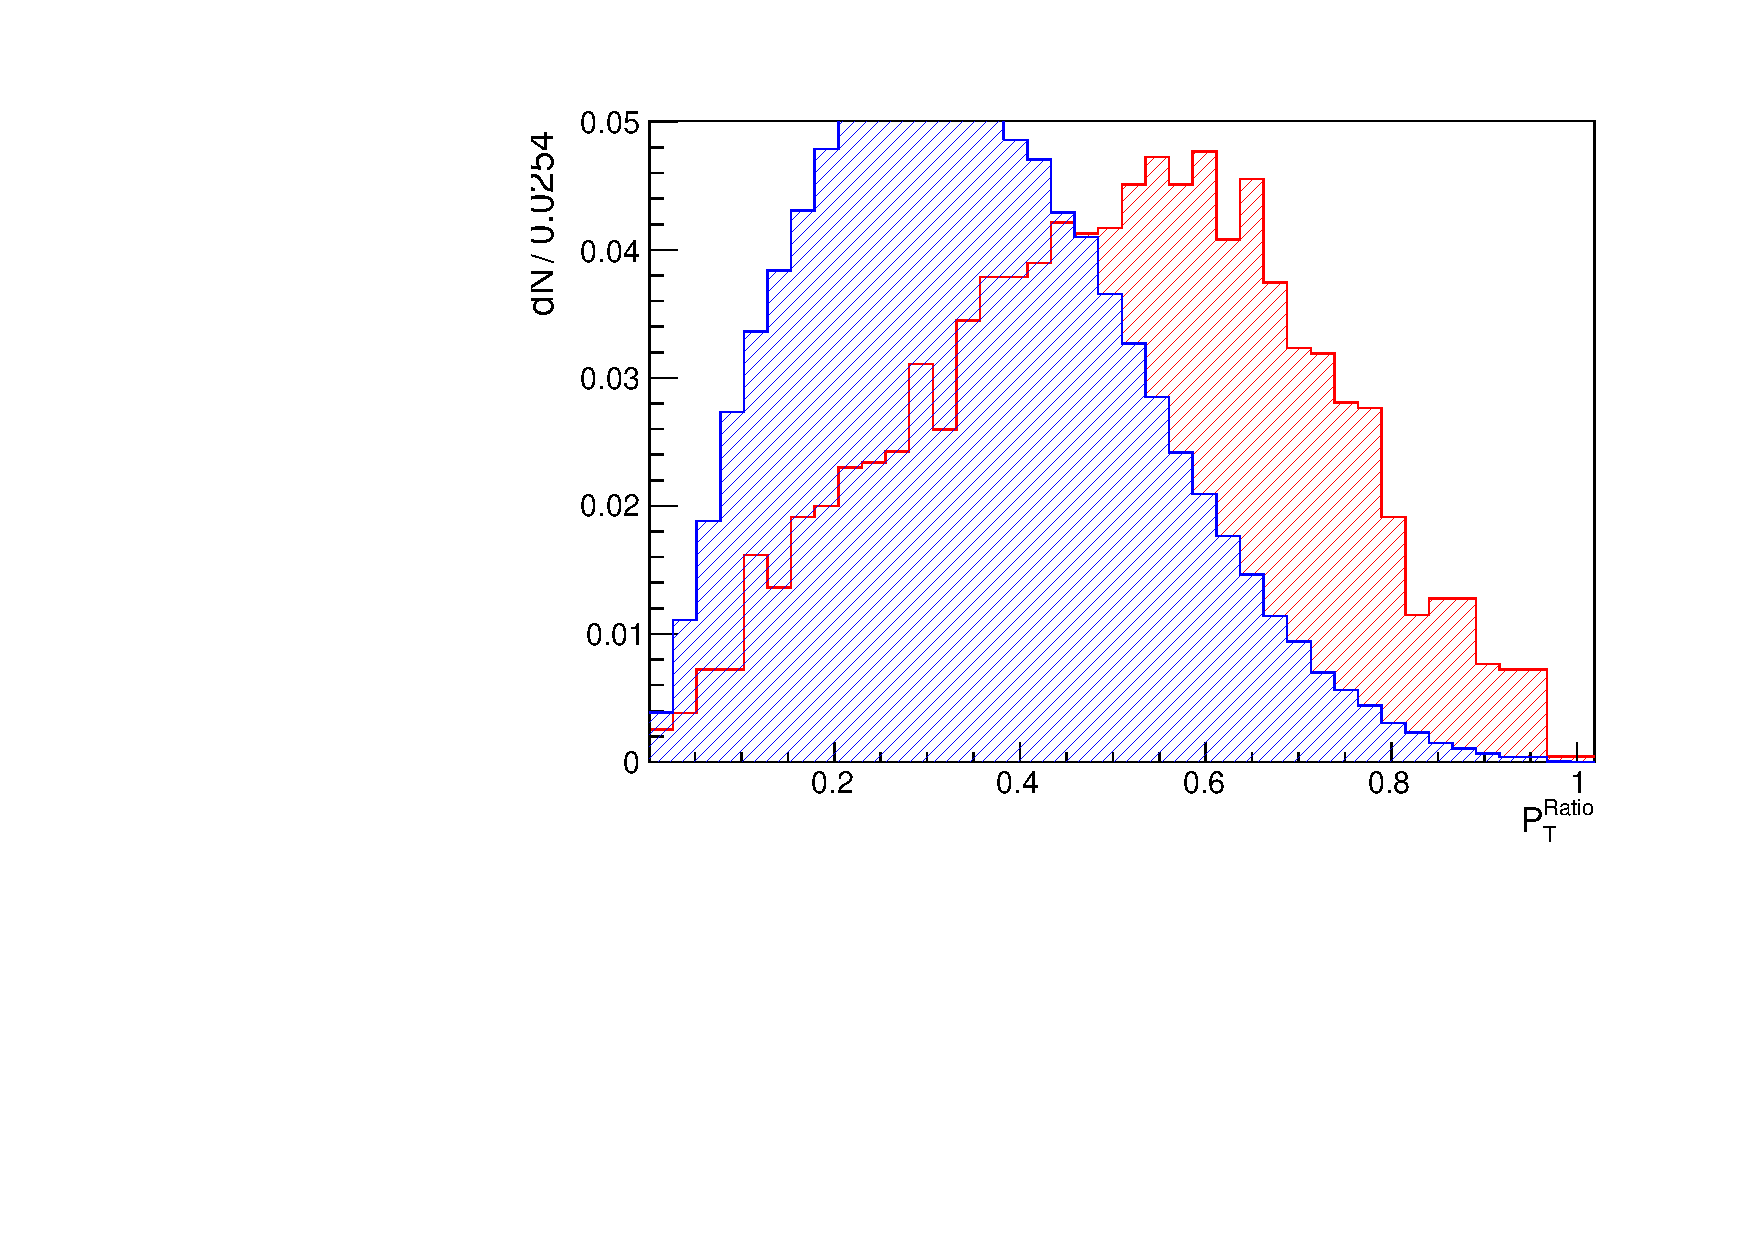
\includegraphics[width=0.49\textwidth]{images/Run1/ThSumPTVecPT.pdf}
     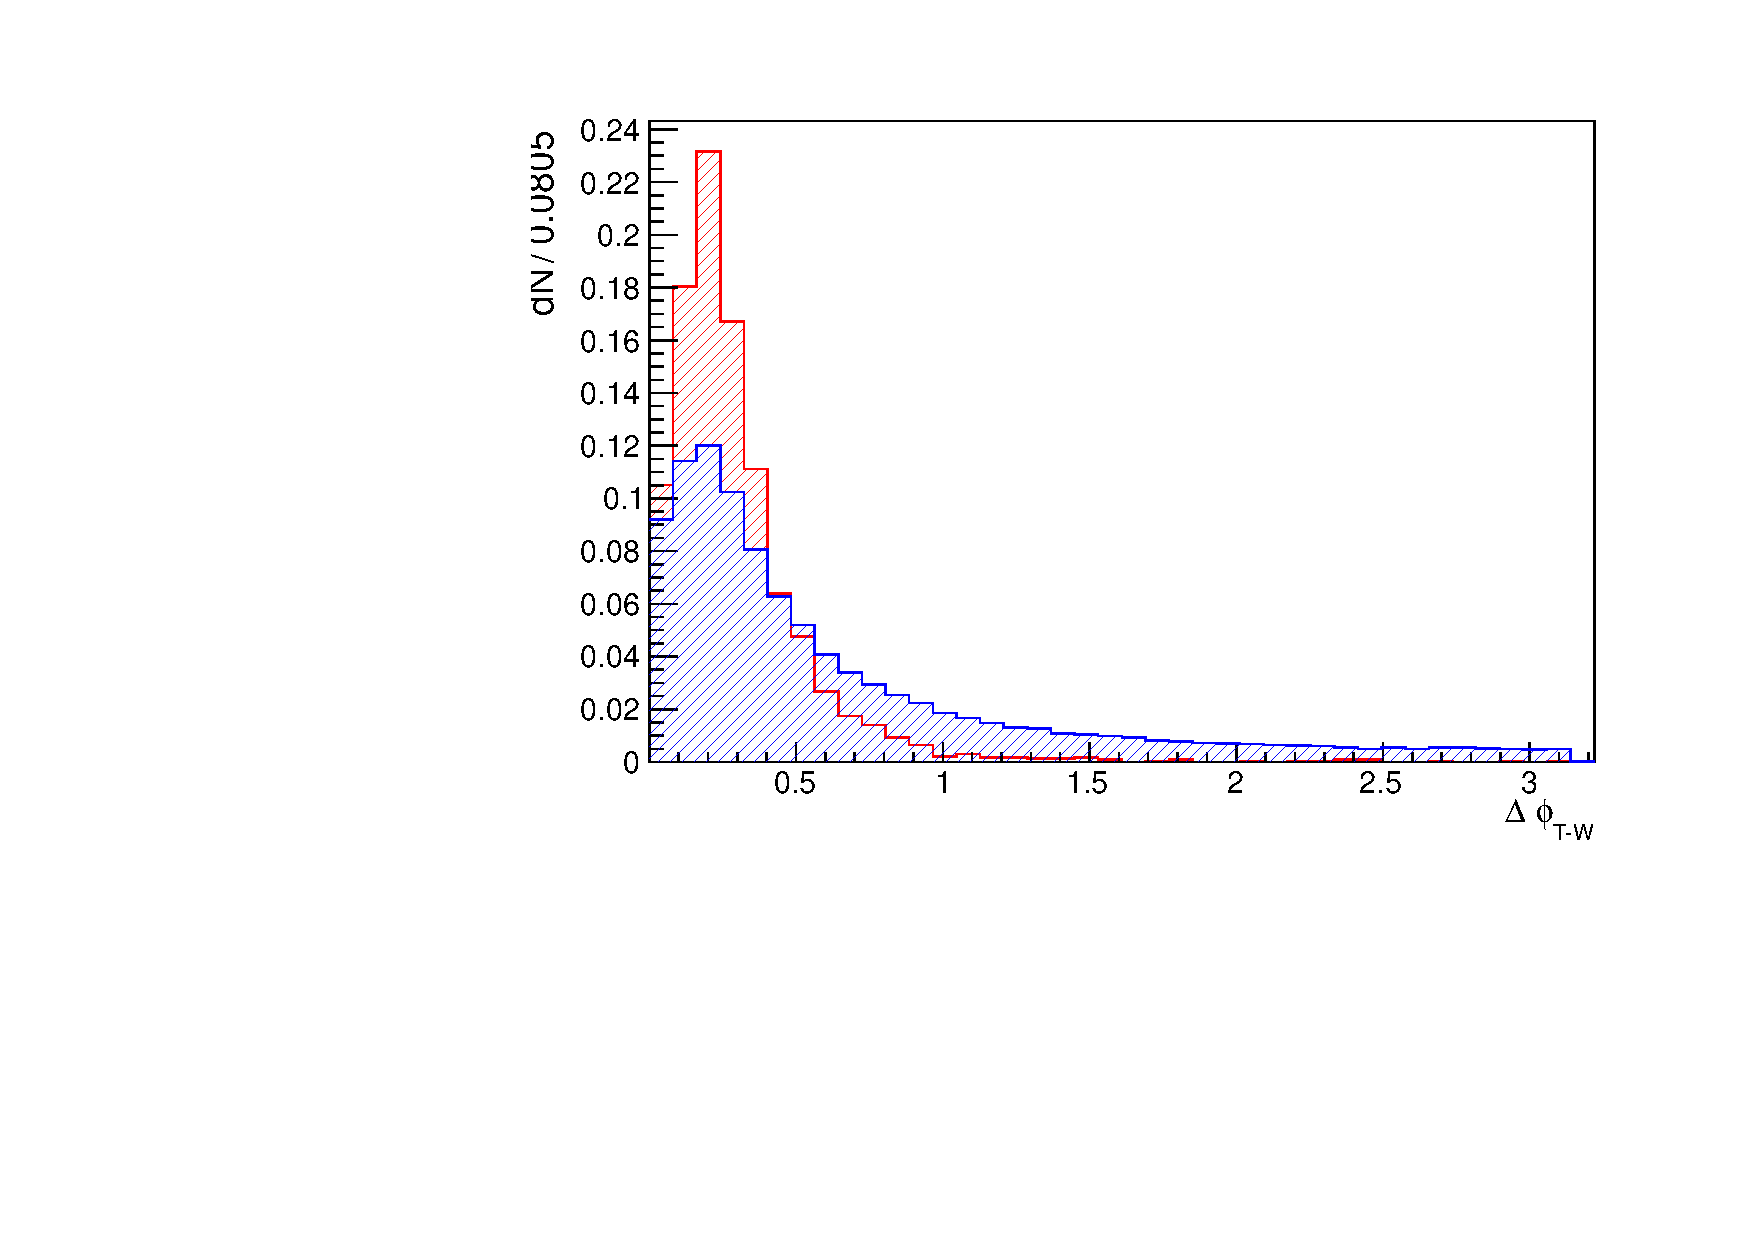
\includegraphics[width=0.49\textwidth]{images/Run1/AnThWh.pdf}
    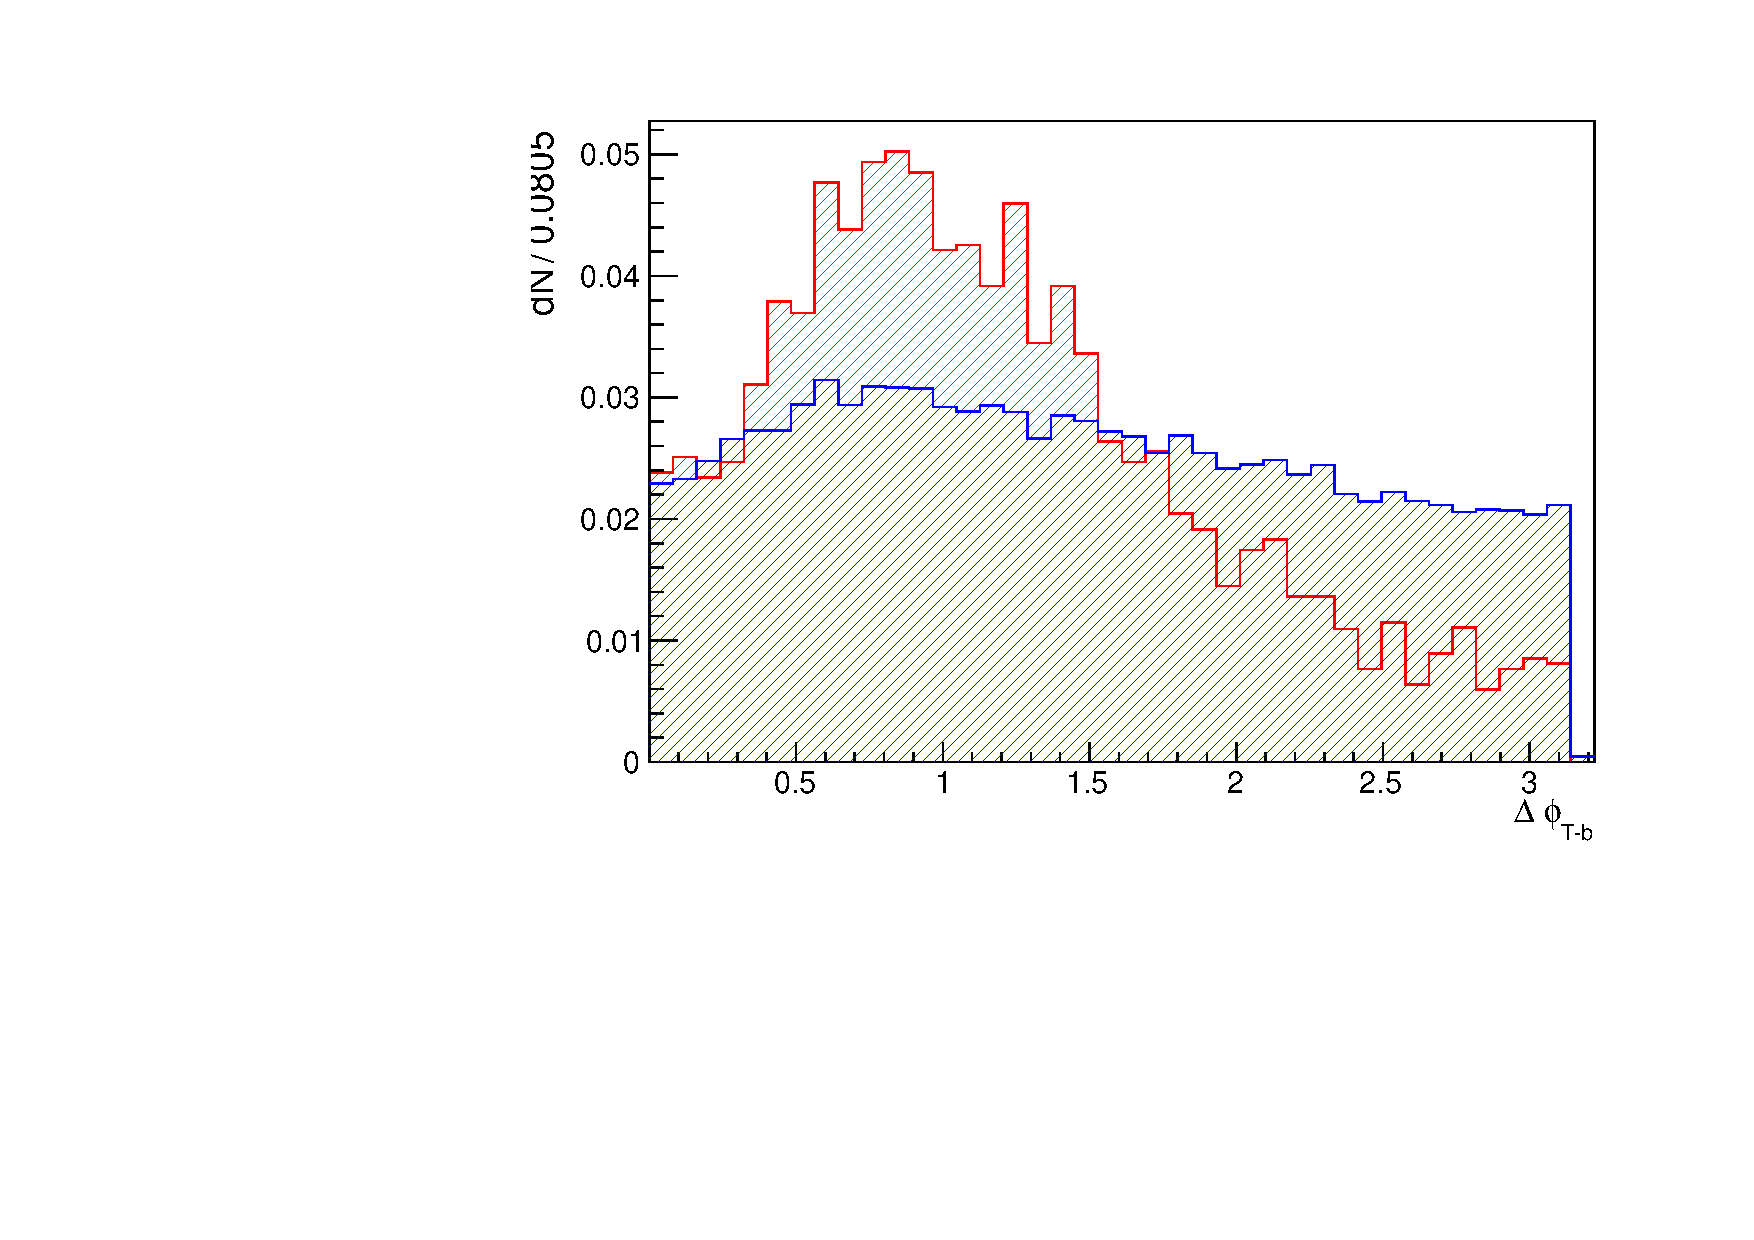
\includegraphics[width=0.49\textwidth]{images/Run1/AnThBh.pdf}
     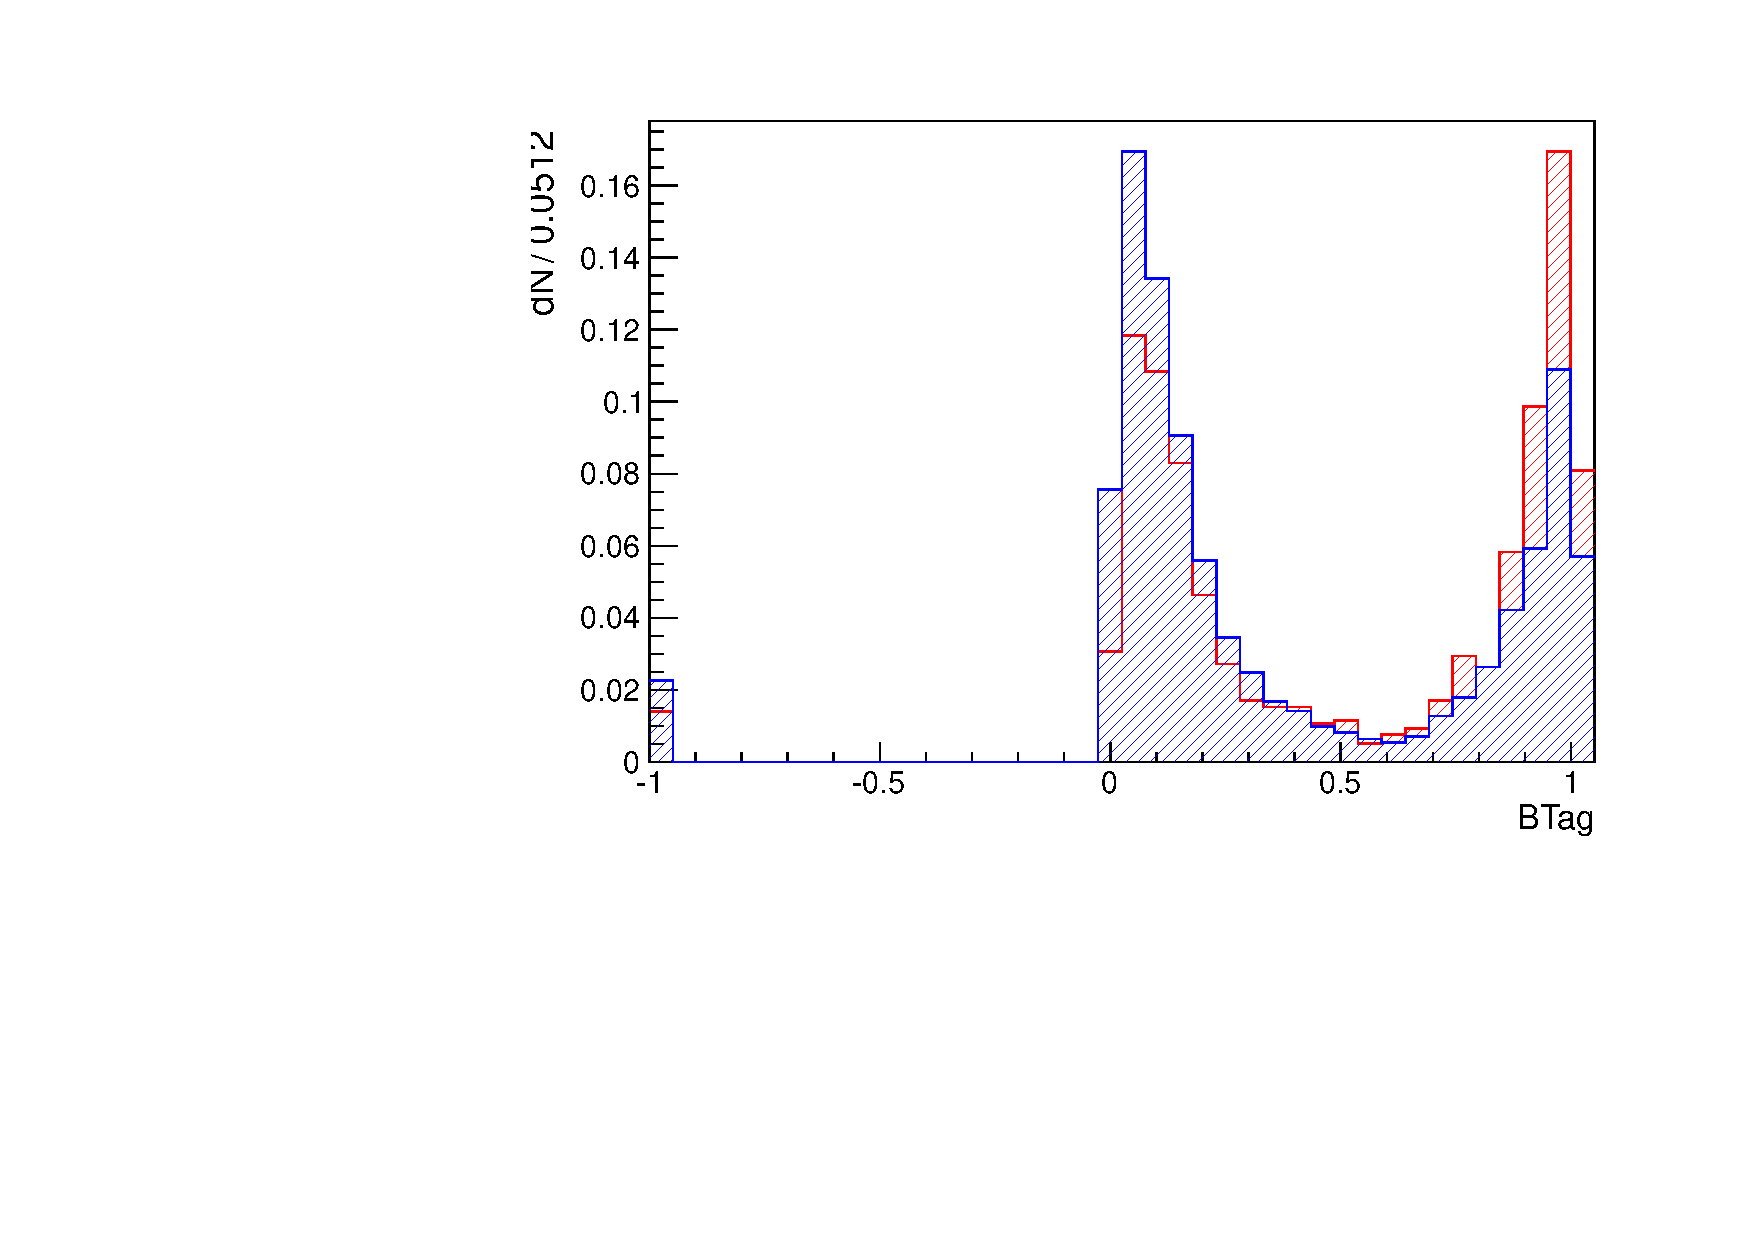
\includegraphics[width=0.49\textwidth]{images/Run1/BTag.pdf}          
    \caption{Input variables into hadronic top quark reconstruction BDT.}
    \label{fig:TopBDTinput}
\end{figure}

% The multi-variate analysis tool chosen to calculate a variable to discriminate between good and bad tri-jet combinations is a BDT. The BDT is described in more detail in Section~\ref{sec:BDT}. 
The distribution of the discriminator values output from the BDT is shown in Fig.~\ref{fig:TopBDToutput} where the features in the shape are caused by the large discriminating power of the tri-jet and di-jet invariant mass. In Fig.~\ref{fig:TopBDToutput} it can be seen in the tri-jet vs BDT output value plot that tri-jet candidates with an invariant mass close to the top mass are associated with larger BDT output values and particularly there is a split in the BDT discriminator value at $\approx -0.5$ which can be seen as the division between the two peaks in the BDT discriminator plot. Tri-jets with an invariant mass $\gtrsim 300$~GeV tend to have BDT discriminator values $< -0.5$.

\begin{figure}[!ht]
\centering
    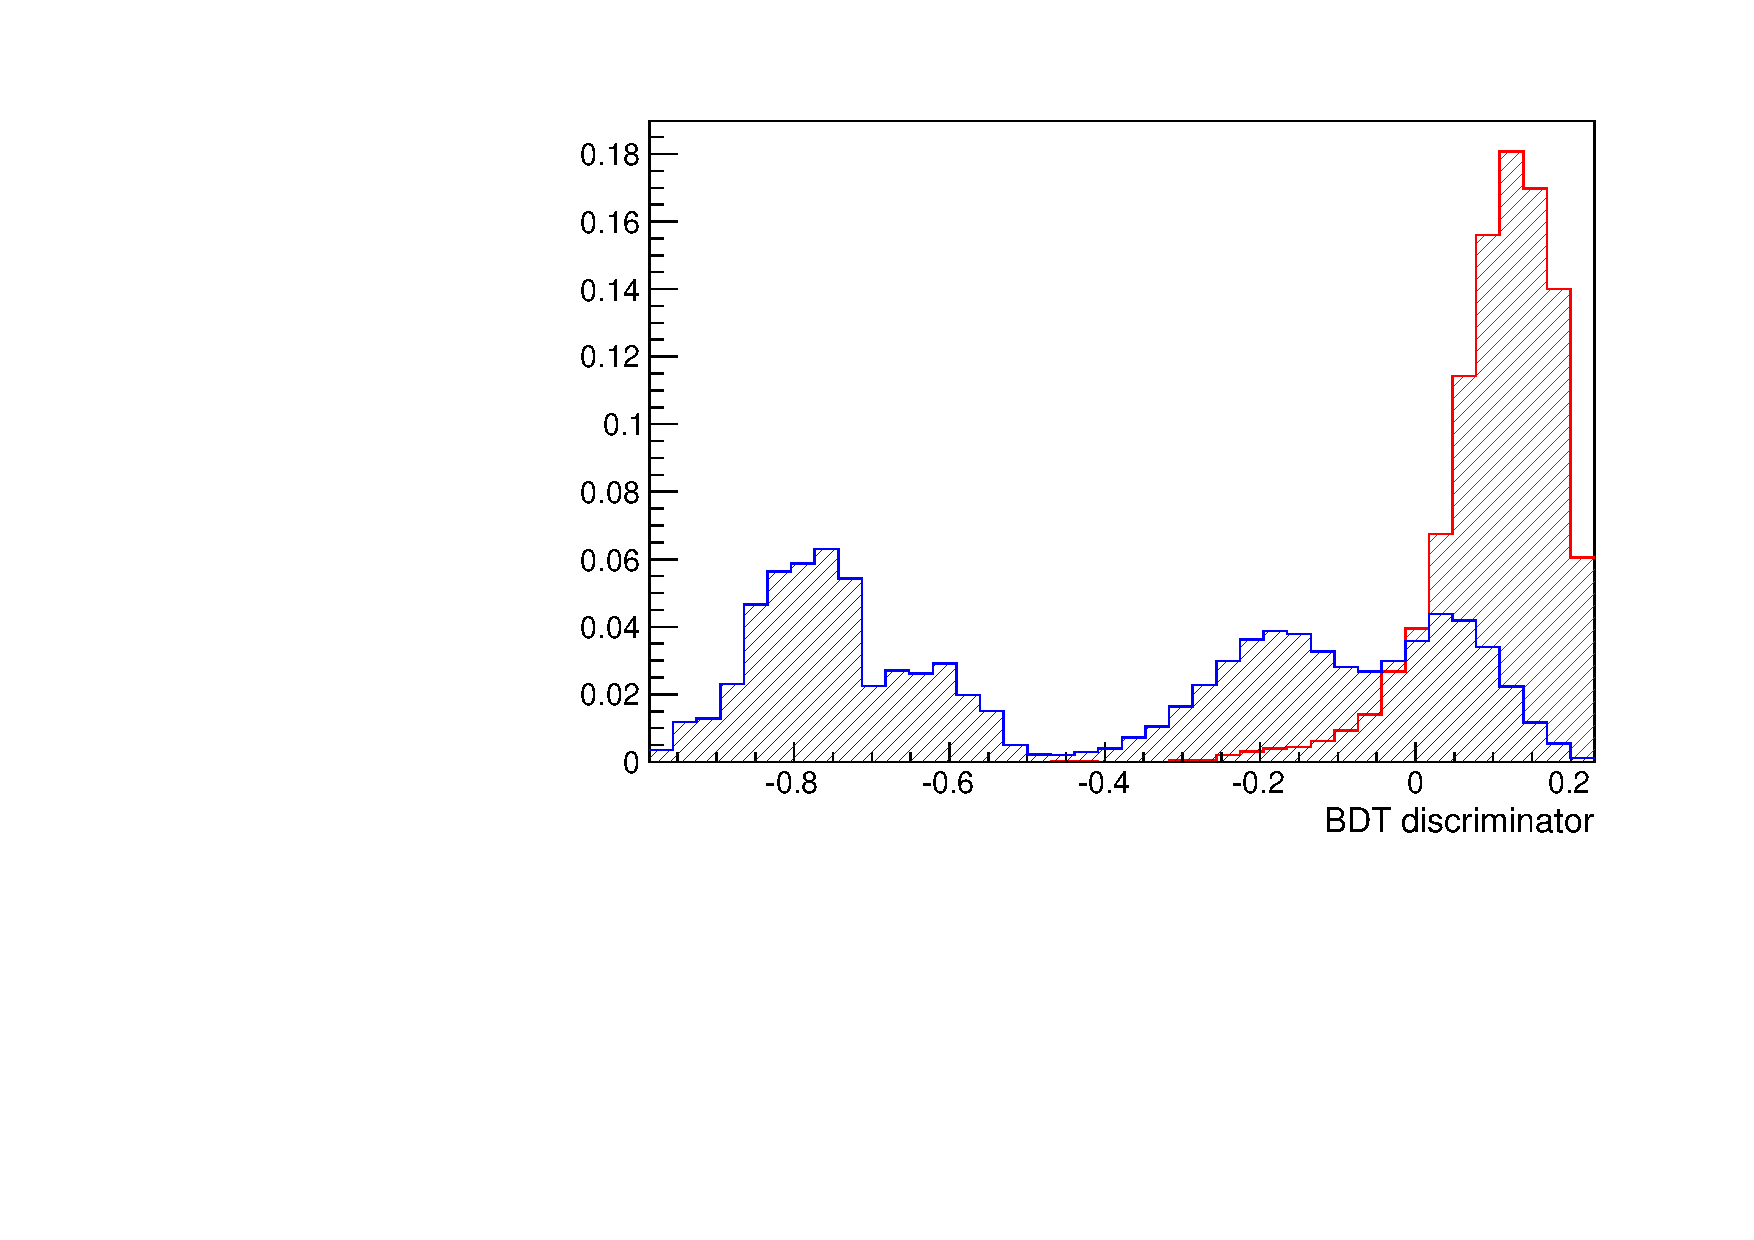
\includegraphics[width=0.49\textwidth]{images/Run1/BDT_Disc.pdf}
    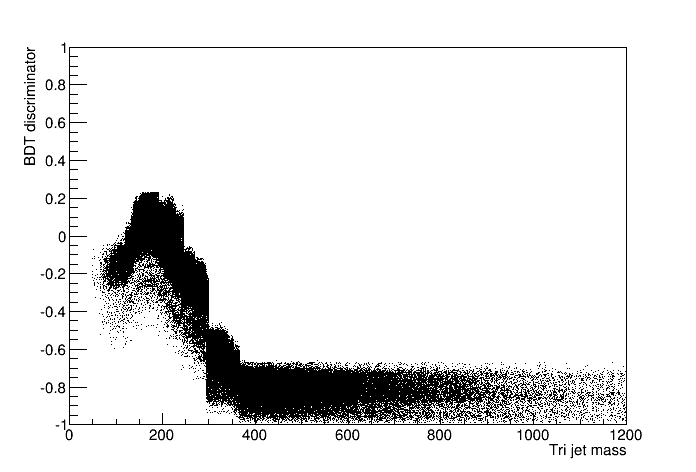
\includegraphics[width=0.49\textwidth]{images/Run1/TrijetmassVsBDT.png}
    \caption{Output discriminator variable from top quark reconstruction BDT (left) and tri-jet mass vs BDT score (right)}
    \label{fig:TopBDToutput}
\end{figure}

\subsubsection*{BDT$_{tri-jet2}$}
% Multitopness is defined to be the BDT discriminator value of the second highest ranking tri-jet after the first highest-ranking tri-jet has been removed from the collection and the remaining jets have been passed through the BDT again. The multitopness value should have values close to 1 for events where there is a second reconstructible top and a value close to -1 where there is only one reconstructible top which has been removed from the collection and the remaining jets are from ISR or FSR. 
The distributions of the BDT$_{tri-jet2}$ variable are shown in Fig.~\ref{fig:Multitopness} for the muon and electron channel. It can be seen that the data and simulation agree well. There is some difference between the shape of the signal and background distributions which can be exploited by the event-level BDT.
%The interesting features in the distributions shape come from the  BDT. 
%The two strongest variables, the tri-jet invariant mass and the di-jet invariant mass, split the dataset sharply into two and then four main sections.

\begin{figure}[!ht]
    \includegraphics[width=0.49\textwidth]{images/Run1/MultiTopness_Mu.pdf}
    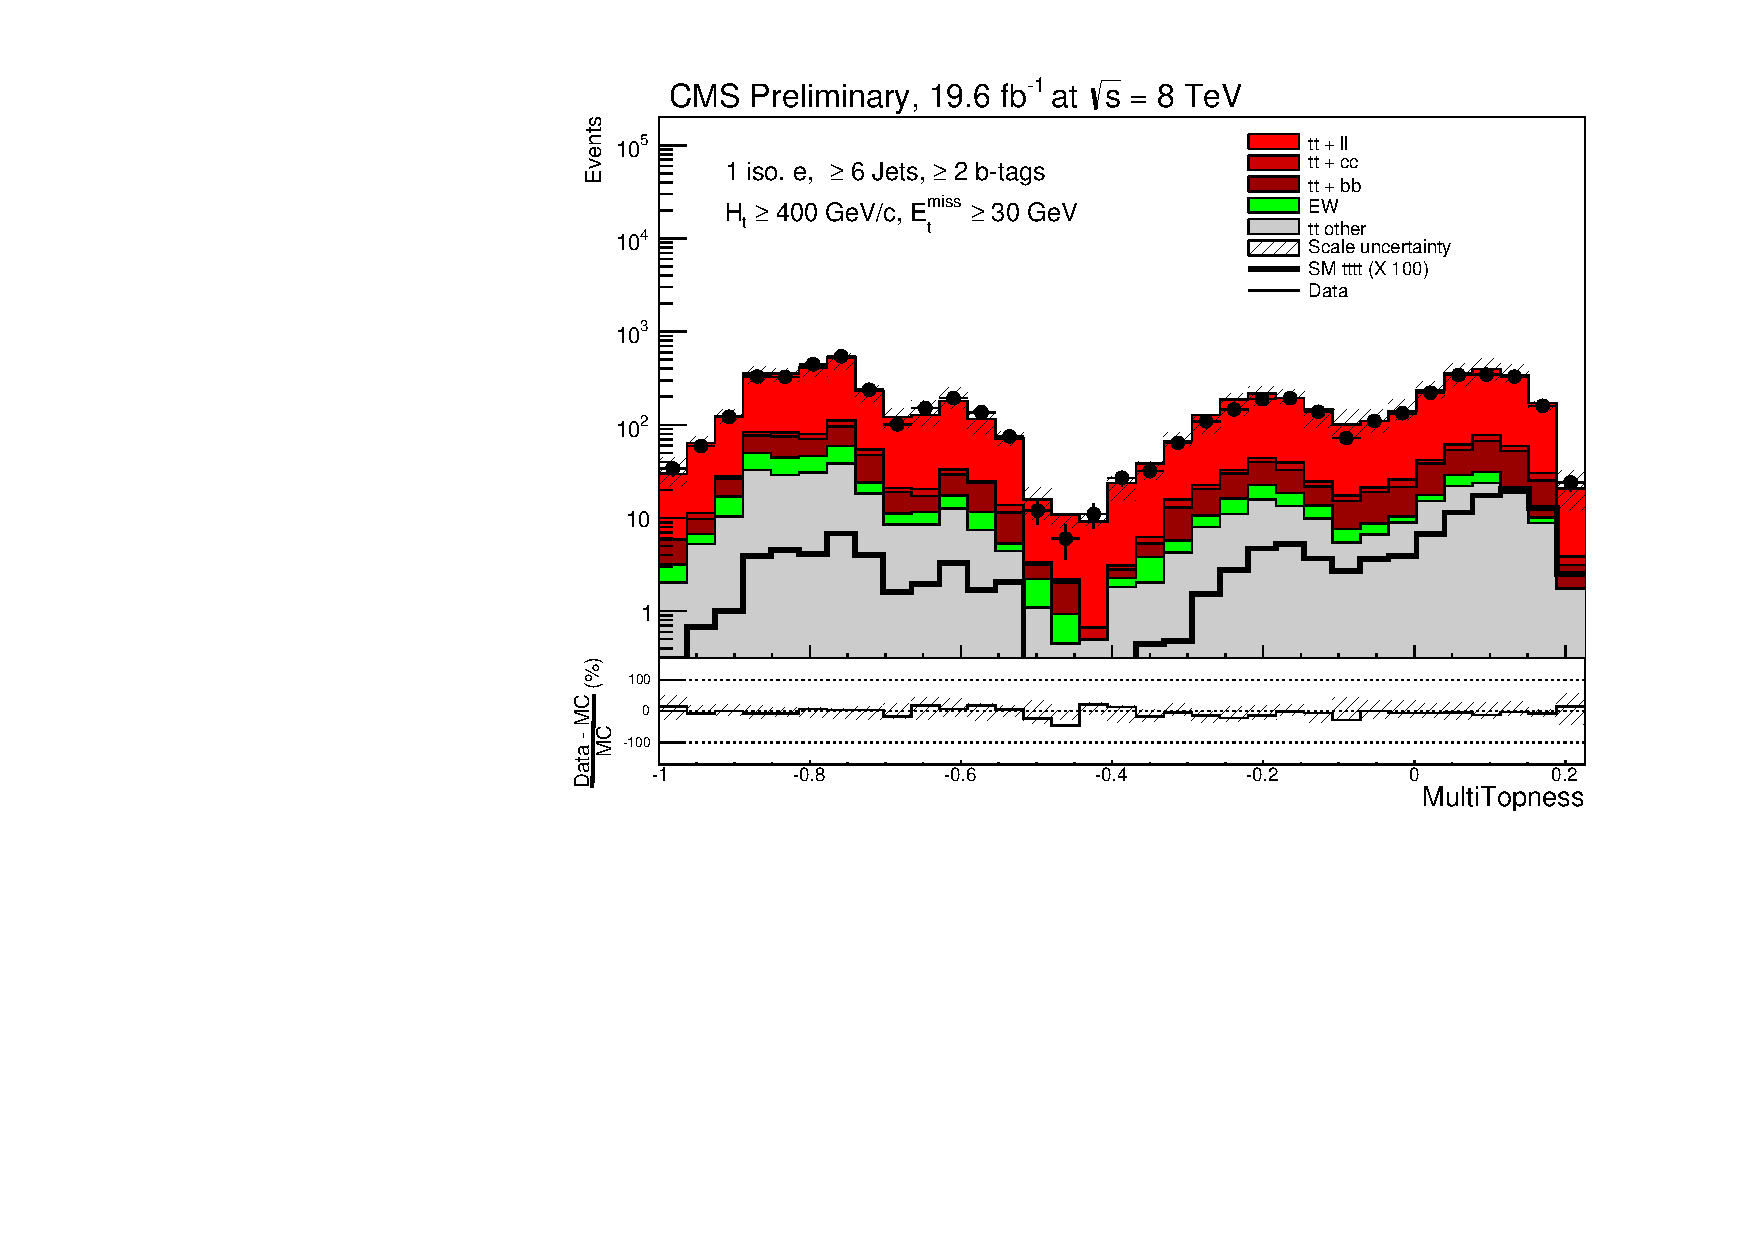
\includegraphics[width=0.49\textwidth]{images/Run1/MultiTopness_e.pdf}
    \caption{BDT$_{tri-jet2}$ in data and simulation for $\mu$ + jets (right) and e + jets (left).}
    \label{fig:Multitopness}
\end{figure}

\subsubsection*{Reduced Event Variables}
% New event variables are constructed from removing the highest ranking tri-jet from the jets collection to created a reduced event. These reduced event variables exploit the fact the \ttbar events should only have softer jets remaining from ISR and FSR, whereas \tttt events should have ore energetic jets from the two additional hadronic top quarks.

% \textbf{\HTX} - This is the \HT of the reduced event.\\
% \textbf{\sumjetmassX} - Invariant mass of all jets contained in the reduced event.

Plots for the \HTX and \sumjetmassX reduced variables, which are derived from the reduced event where jets from the highest ranked hadronic top quark candidate are removed, can be seen in Figs~\ref{fig:HTX},~\ref{fig:sumjetmassX}. These variables have excellent agreement between data and simulation and it is apparent, particularly in the \HTX distribution, that these variables will provide some discrimination power in the event-level BDT.

\begin{figure}[!ht]
    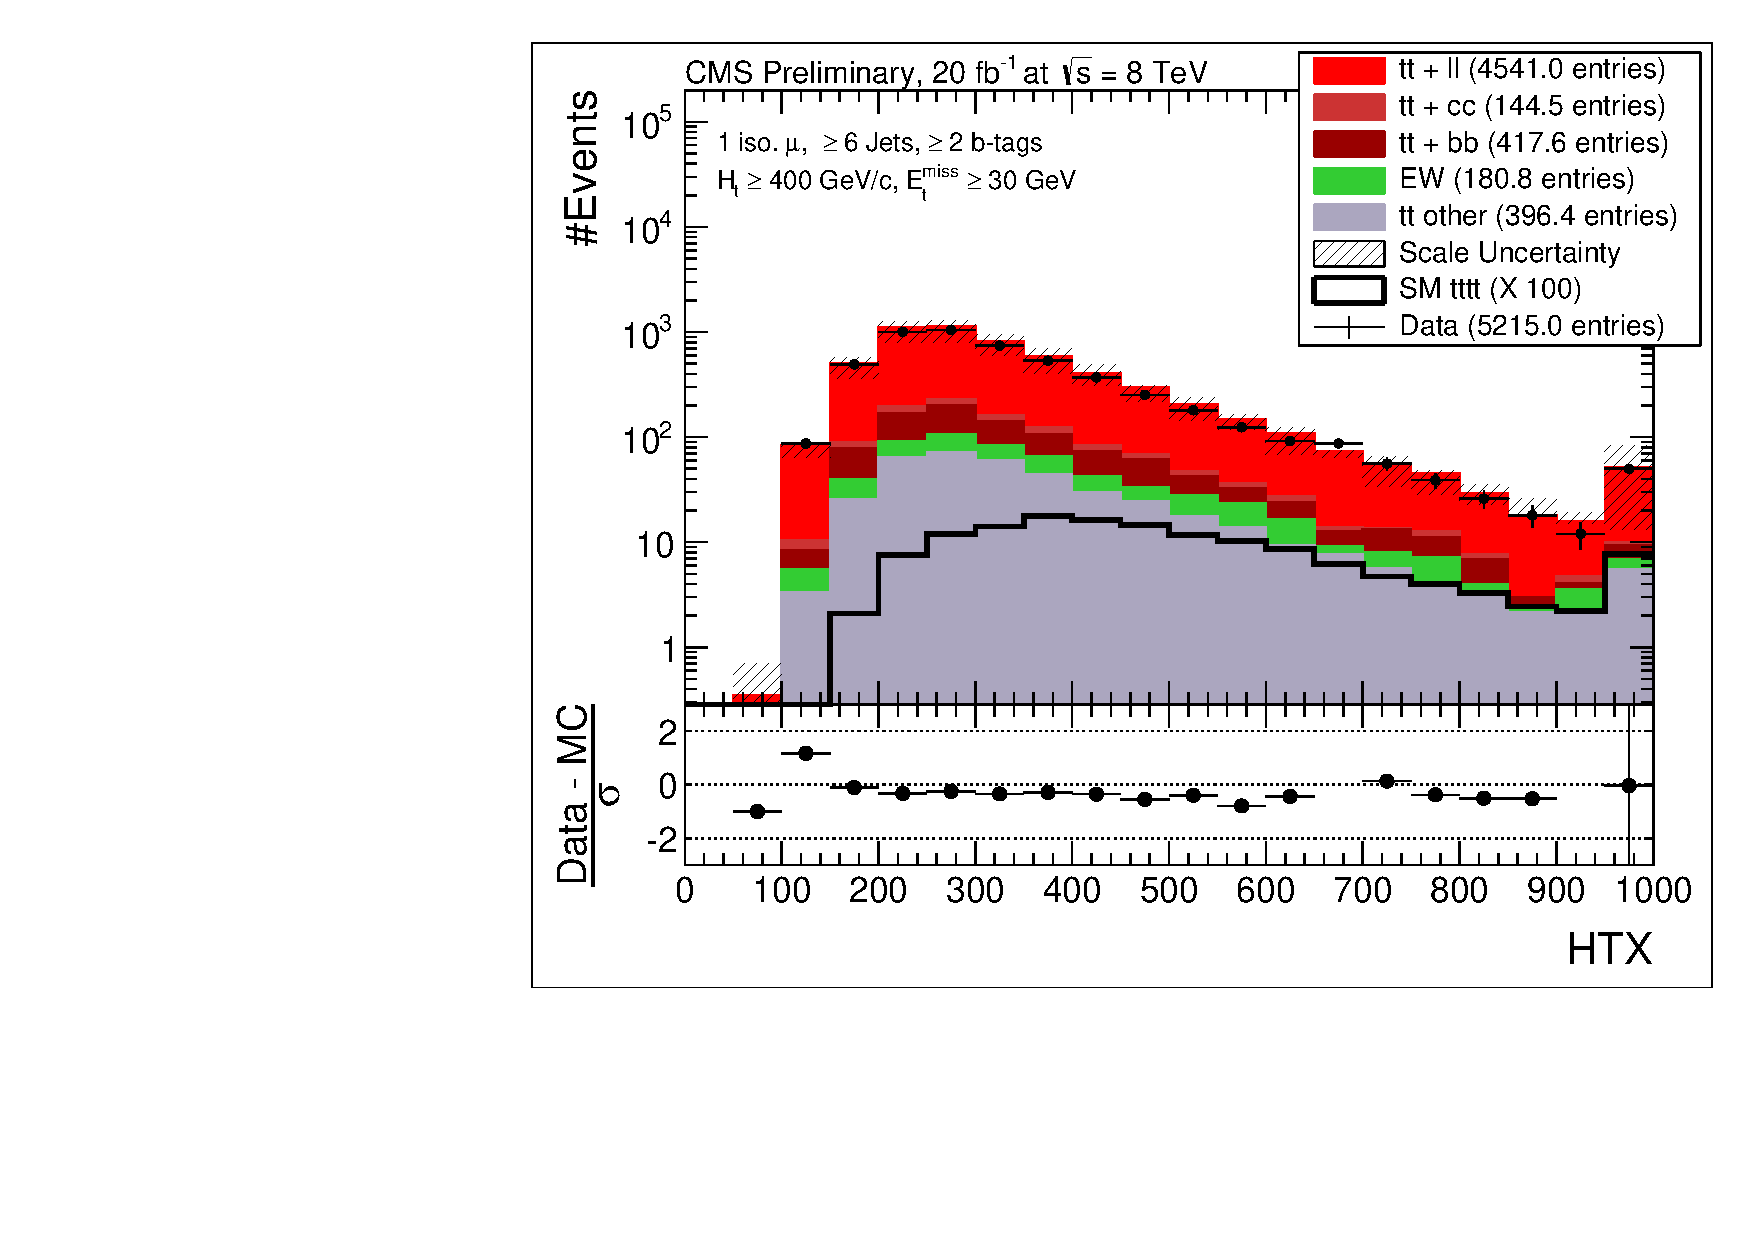
\includegraphics[width=0.49\textwidth]{images/Run1/HTX_StackLogY_Mu.pdf}
    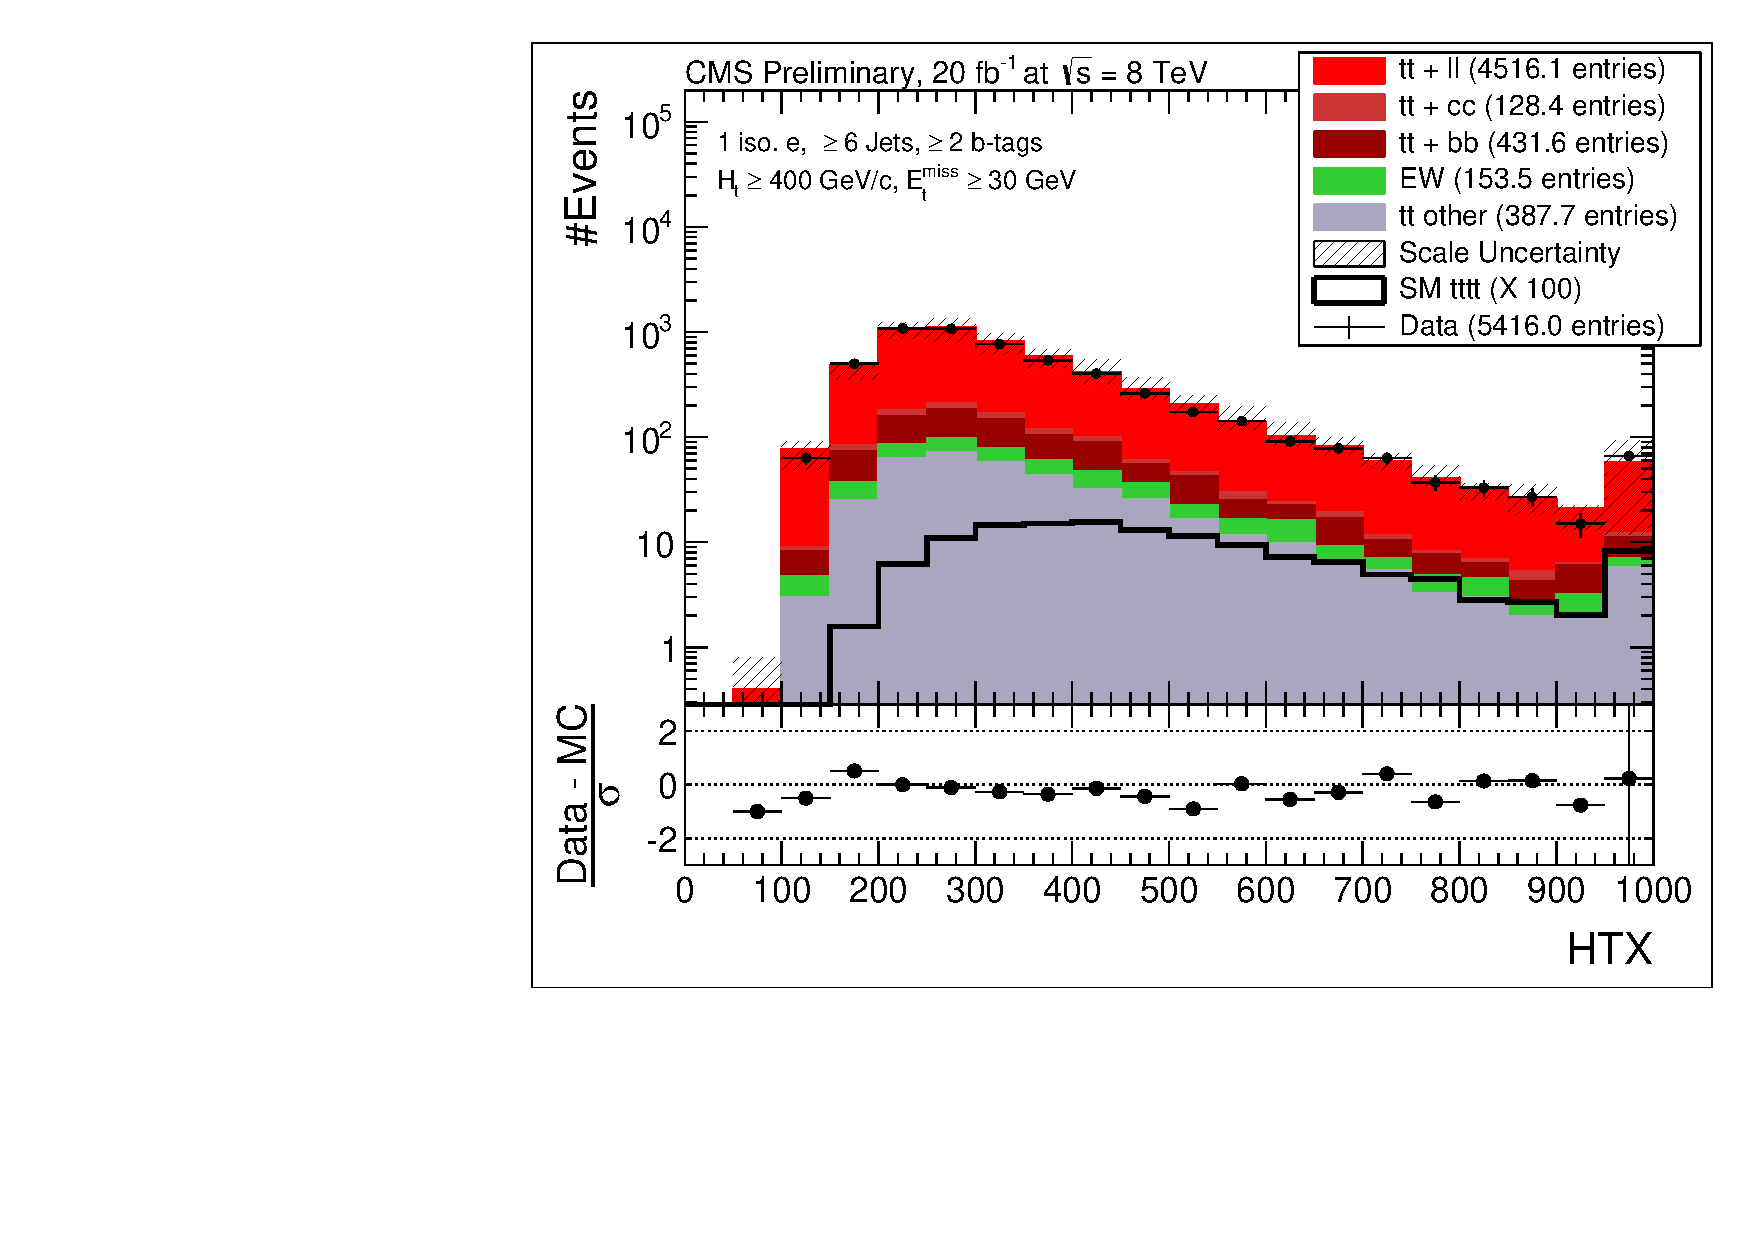
\includegraphics[width=0.49\textwidth]{images/Run1/HTX_StackLogY_e.pdf}
    \caption{\HTX for $\mu$ + jets (right) and e + jets (left).}
    \label{fig:HTX}
\end{figure}

\begin{figure}[!ht]
    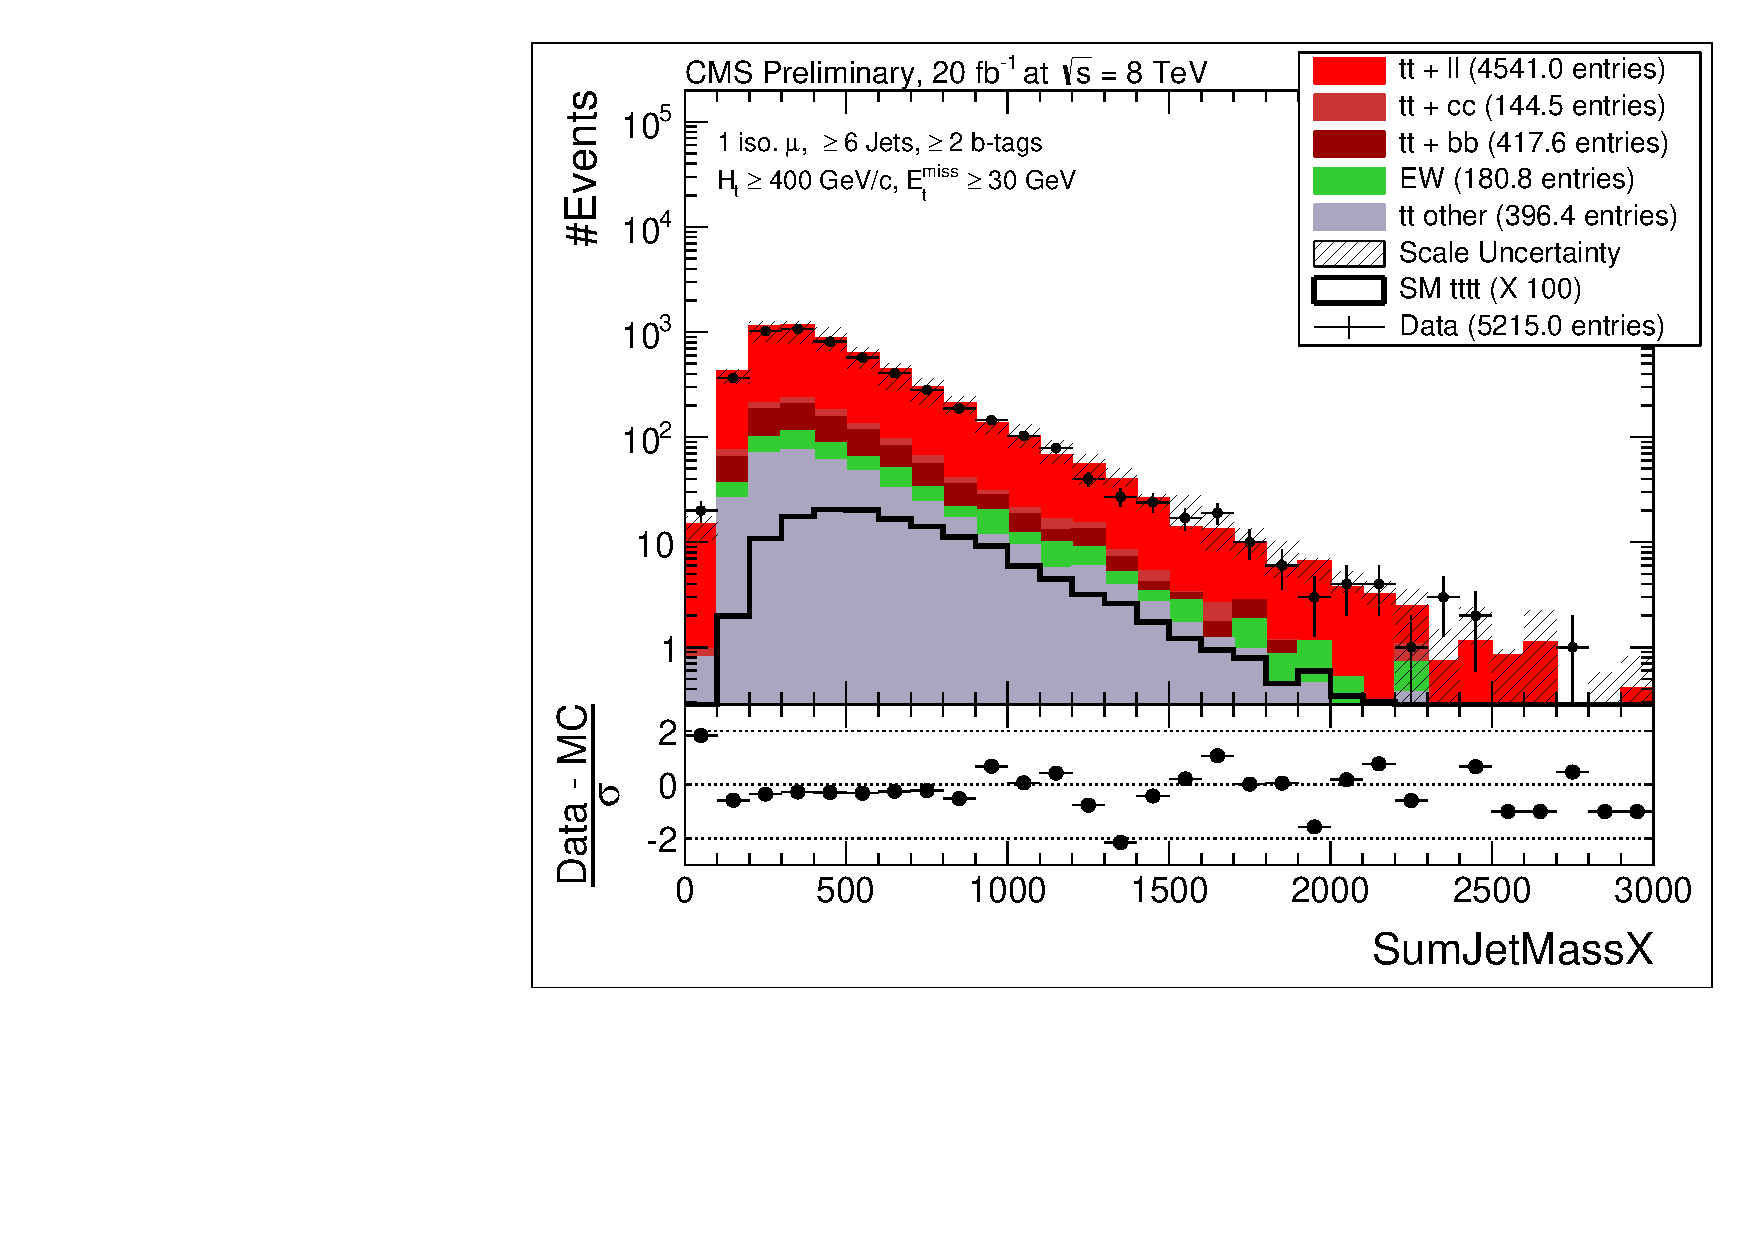
\includegraphics[width=0.49\textwidth]{images/Run1/SumJetMassX_StackLogY_Mu.pdf}
    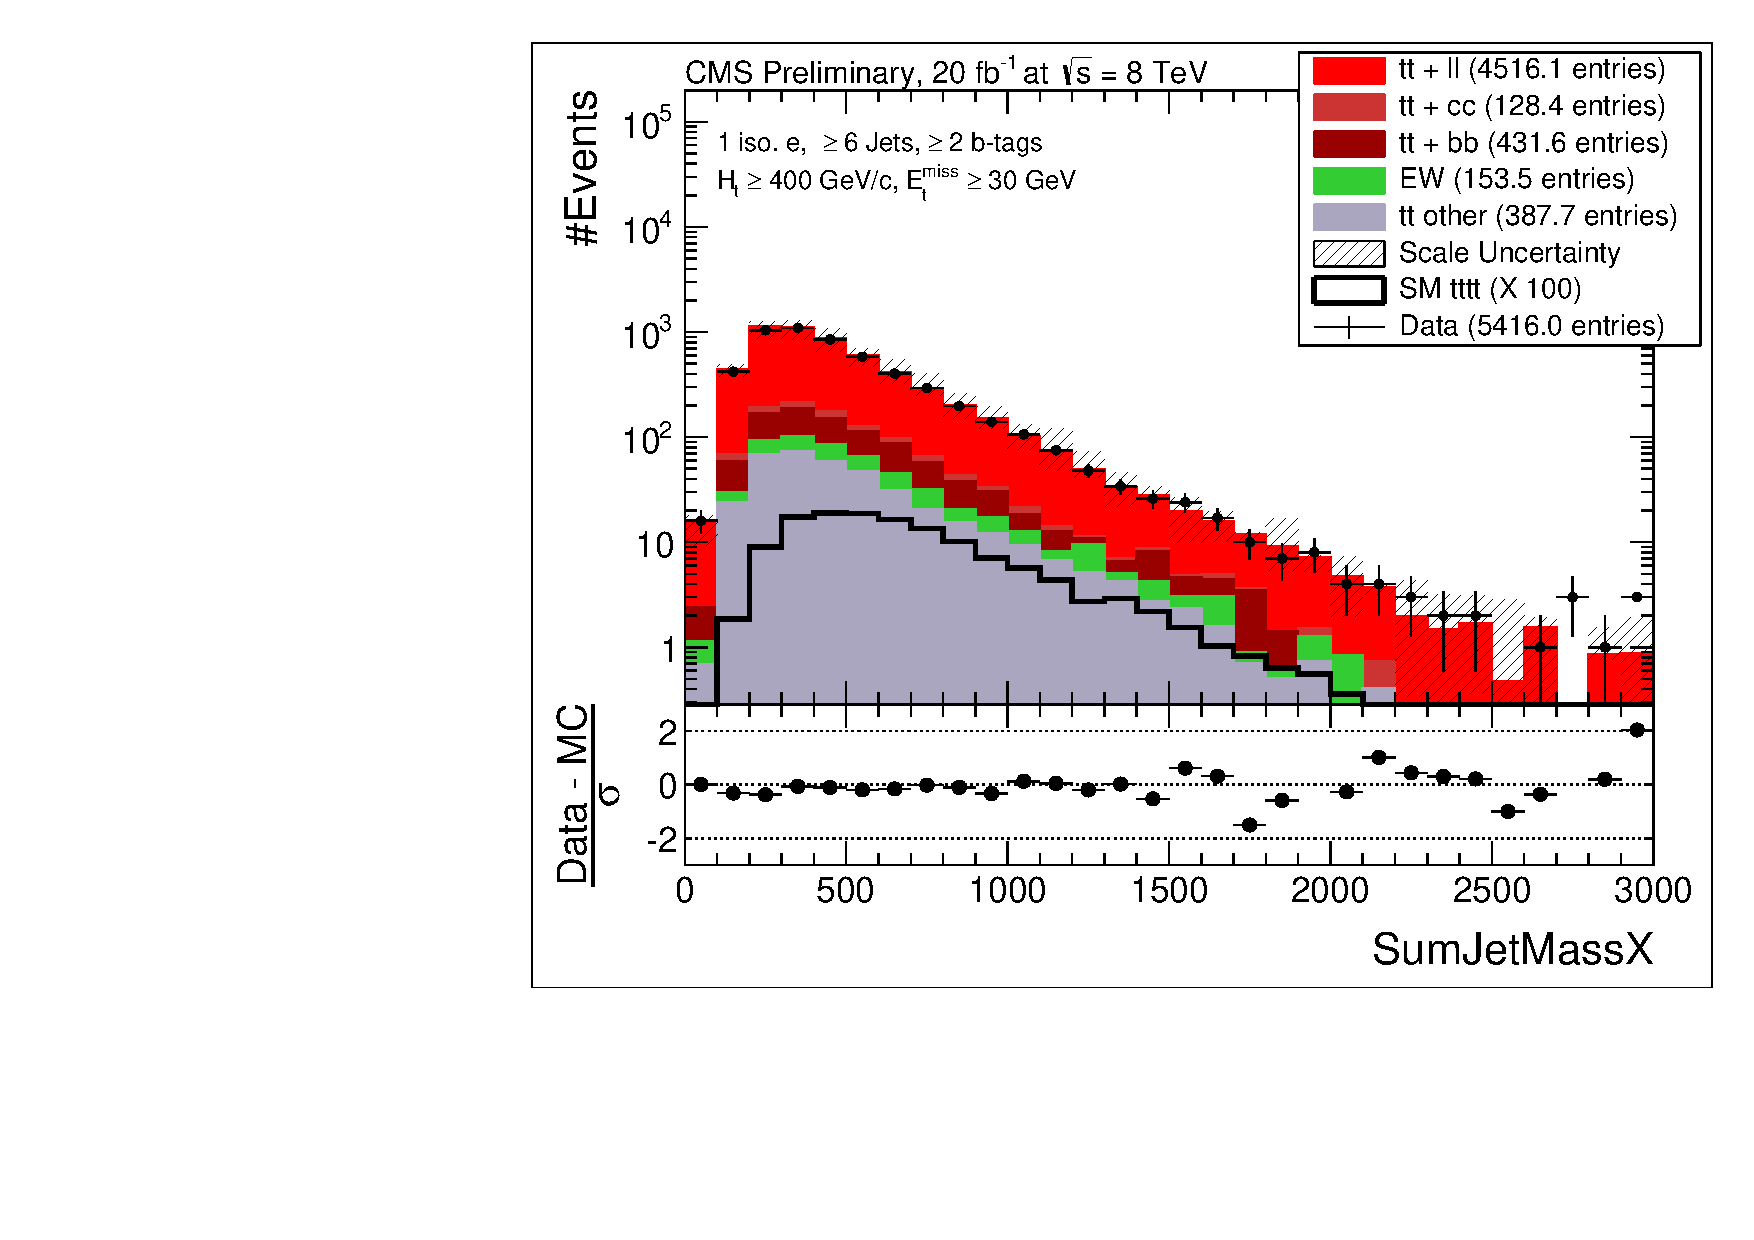
\includegraphics[width=0.49\textwidth]{images/Run1/SumJetMassX_StackLogY_e.pdf}
    \caption{\sumjetmassX for $\mu$ + jets (right) and e + jets (left).}
    \label{fig:sumjetmassX}
\end{figure}

% \subsection{b-jet content}
% \label{sec:bottomContent}
% Top quarks decay almost exclusively into bottom quarks by \cPqt $\rightarrow$ \cPqb \Wplus or \cPaqt $\rightarrow$ \cPaqb \Wminus. Therefore, it should be possible to use the number of bottom quarks in the event to distinguish between \tttt events, which should have four bottom quarks in comparison to \ttbar + jets events which typically have two bottom quarks. However this variable does not help to distinguish between \tttt and \ttbb as \ttbb will also have four bottom quarks in the final state. Also \ttbar + jets may have additional bottom quarks arising from the ISR or FSR. 


\subsection{Event activity and b-jet content variables chosen for the event-level BDT}
\label{sec:eventActivity}
% Many variables can be derived by utilising the fact that \tttt events can have up to 10 hard jets whereas \ttbar events should only have up to 4 hard jets. This difference in hadronic activity is exploited by forming the following variables:\\
% \textbf{\njets} - The number of jets is an obvious variable for distinguishing between \tttt and \ttbar. It can be seen in Fig.~\ref{fig:datasimnjets}. \\
% \textbf{\HTb} - The scalar sum of the \pt of the b-tagged jets in the event. Bottom quarks which come from top quark decays tend to have higher \pt than bottom quarks which come from gluon splitting and other processes. As \tttt events should contain four b-quarks which come from top decays and \ttbar events contain two b-quarks from top decays, this variable should be larger for \tttt events, as can be seen in Fig.~\ref{fig:HTb}.\\
% \textbf{Centrality} - This is defined as the ratio of the \HT in the event to the H in the event, where H is the scalar sum of the total momentum (P) in the event.\\
% \textbf{\HTrat} - This is defined as the ratio of the \HT of the four leading jets to the \HT of the other jets in the event. For \ttbar, which should have only four hard jets, this ratio should be larger than \tttt which should have a value closer to one as the four hardest jets are balanced be additional hard jets in the event. \\
% \textbf{5th jet \pt} - After the four leading hard jets in \ttbar, the 5th jet should have, on average, a lower momentum in \ttbar events than in \tttt events. This can be seen in Fig.~\ref{fig:5thjetpt}.\\
% \textbf{6th jet \pt} - Again, the \pt of the 6th jet in \ttbar events should be, on average, lower than in \tttt where the 6th jet is still coming from a hard process. This can be seen in Fig.~\ref{fig:6thjetpt}.\\

The variables chosen for use in the event-level BDT due to their discrimination power include:
\begin{multicols}{2}
\begin{itemize}
\item \njets
\item \nMtags
\item \HTb
\item Centrality
\item \HTrat
\item 5th jet \pt
\item 6th jet \pt
\item BDT$_{tri-jet2}$
\item \sumjetmassX
\item \HTX
\end{itemize}
\end{multicols}
These variables are fully described in section~\ref{sec:MVAtechniques}. All of the variables in Figures~\ref{fig:HTb}-~\ref{fig:6thjetpt} show good agreement between data and simulation and the discriminating power is quite apparent in the distributions of Centrality and \HTrat in Fig.~\ref{fig:centrality} and Fig.~\ref{fig:HTrat}, respectively. Fig~\ref{fig:datasimnbtags} shows the distribution of \nMtags which again shows good agreement between data and simulation and it can be seen that the \tttt signal is more likely to produce events with a higher number of \nMtags than the background due to having four b-quarks in the final state.


\begin{figure}[!ht]
    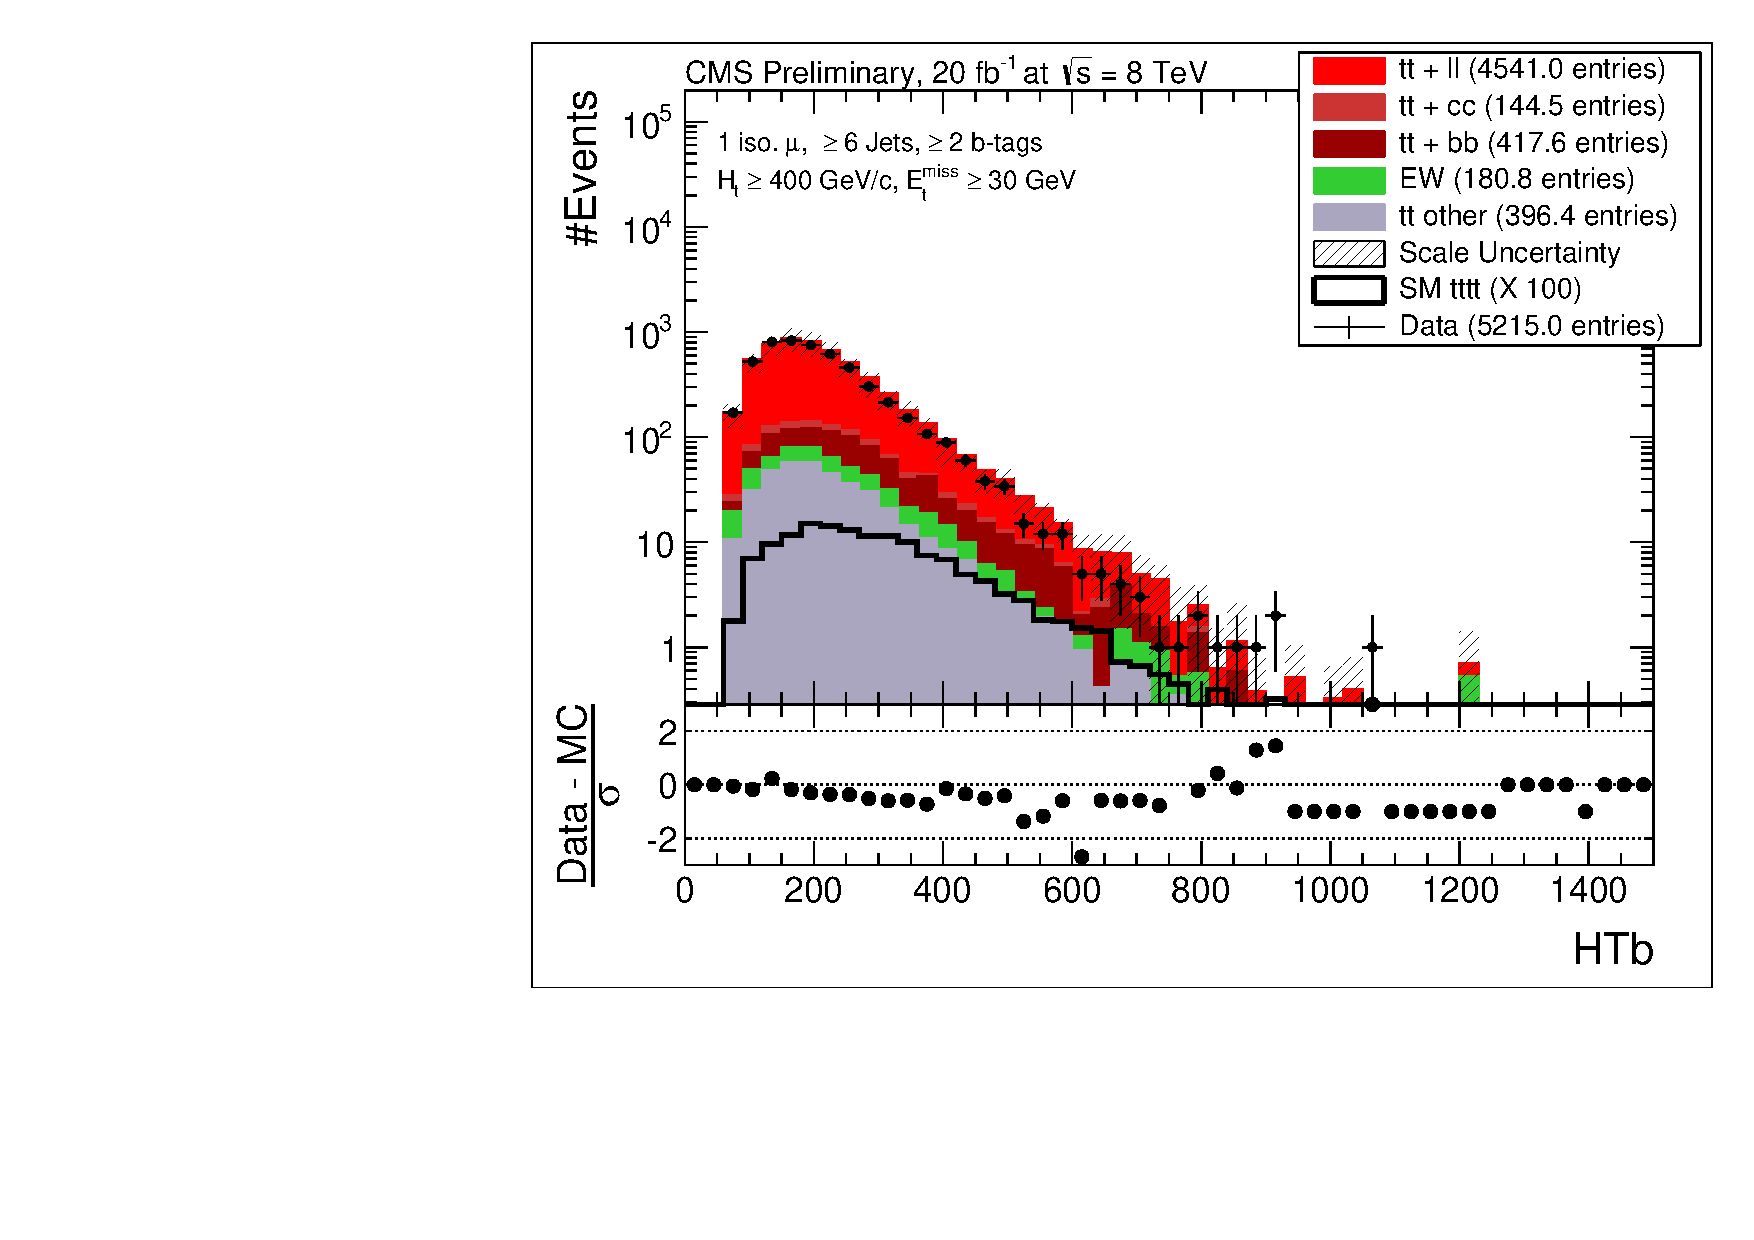
\includegraphics[width=0.49\textwidth]{images/Run1/HTb_SelectedJets_StackLogY_Mu.pdf}
    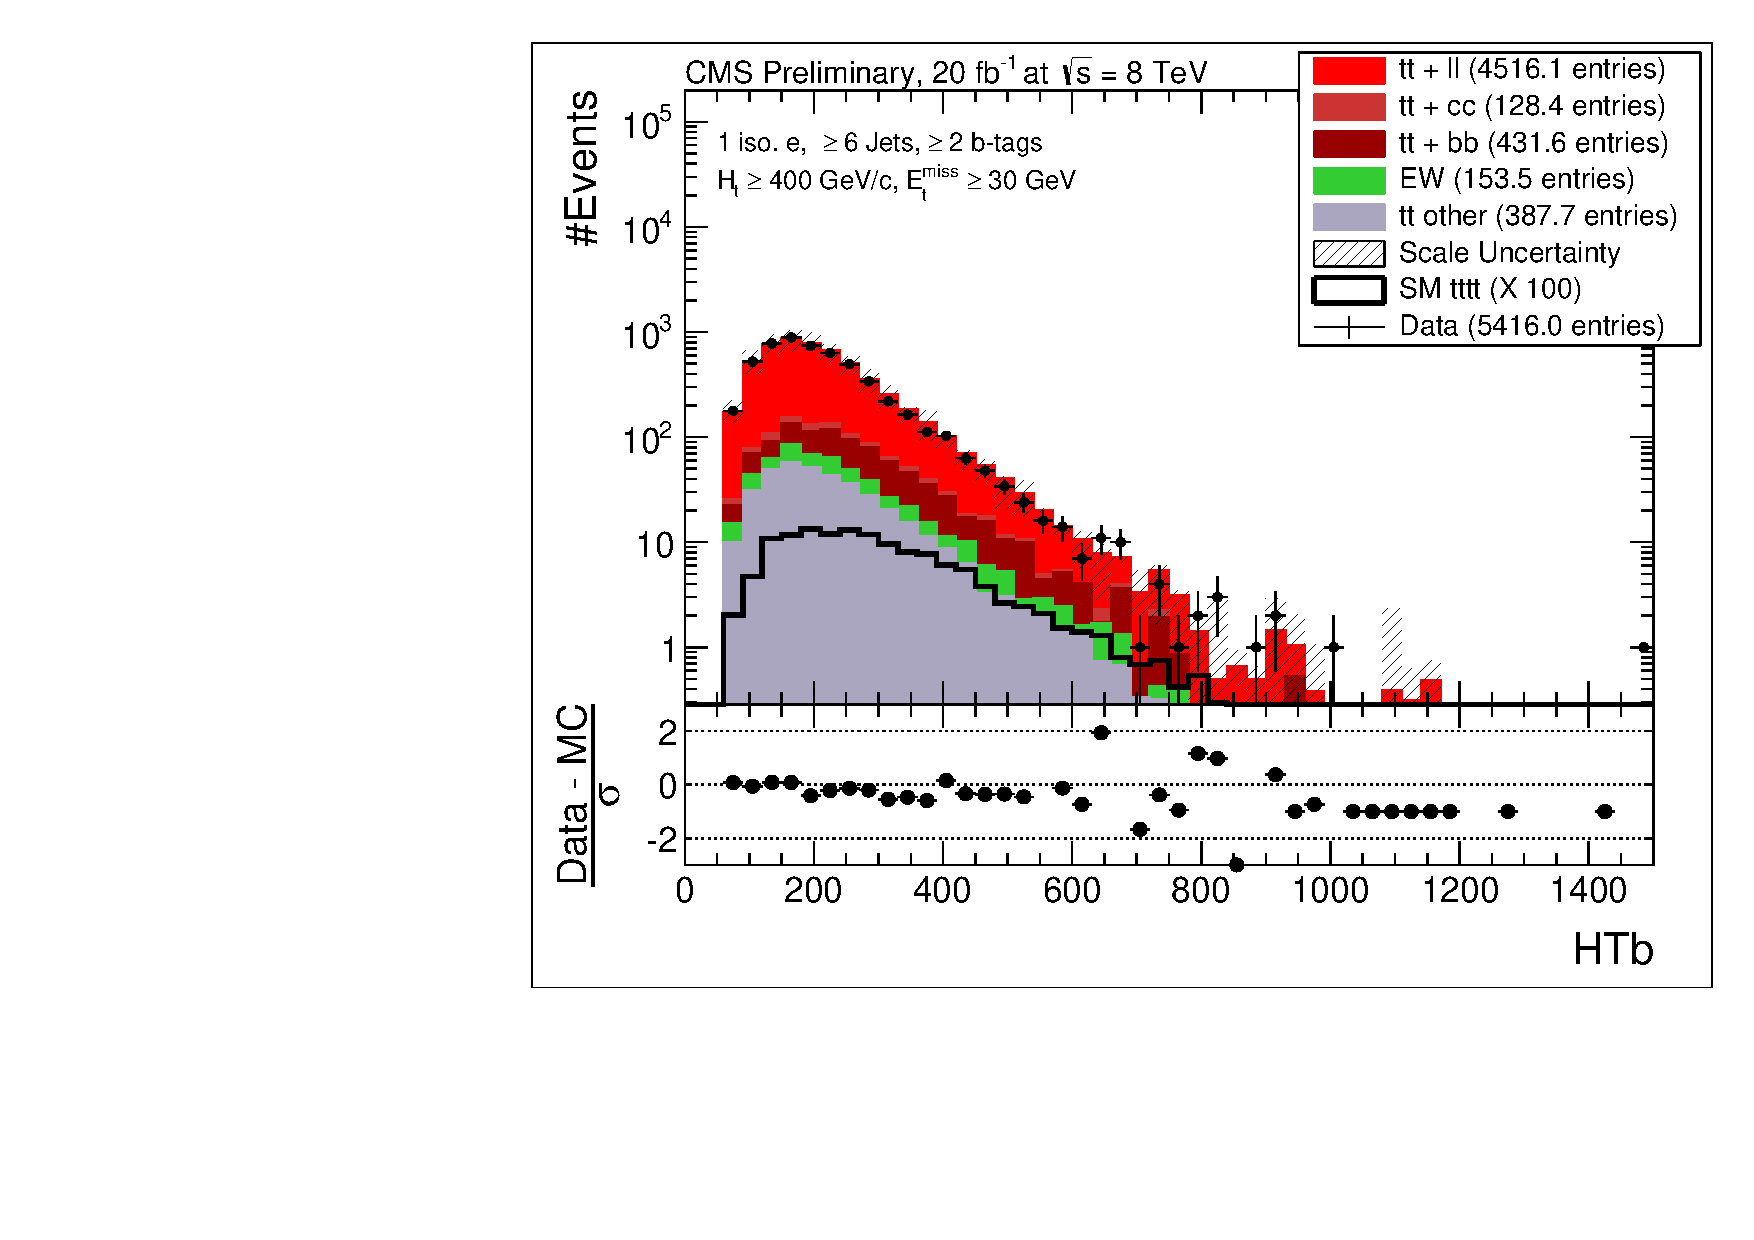
\includegraphics[width=0.49\textwidth]{images/Run1/HTb_SelectedJets_StackLogY_e.pdf}
    \caption{\HTb for $\mu$ + jets (right) and e + jets (left).}
    \label{fig:HTb}
\end{figure}

\begin{figure}[!ht]
    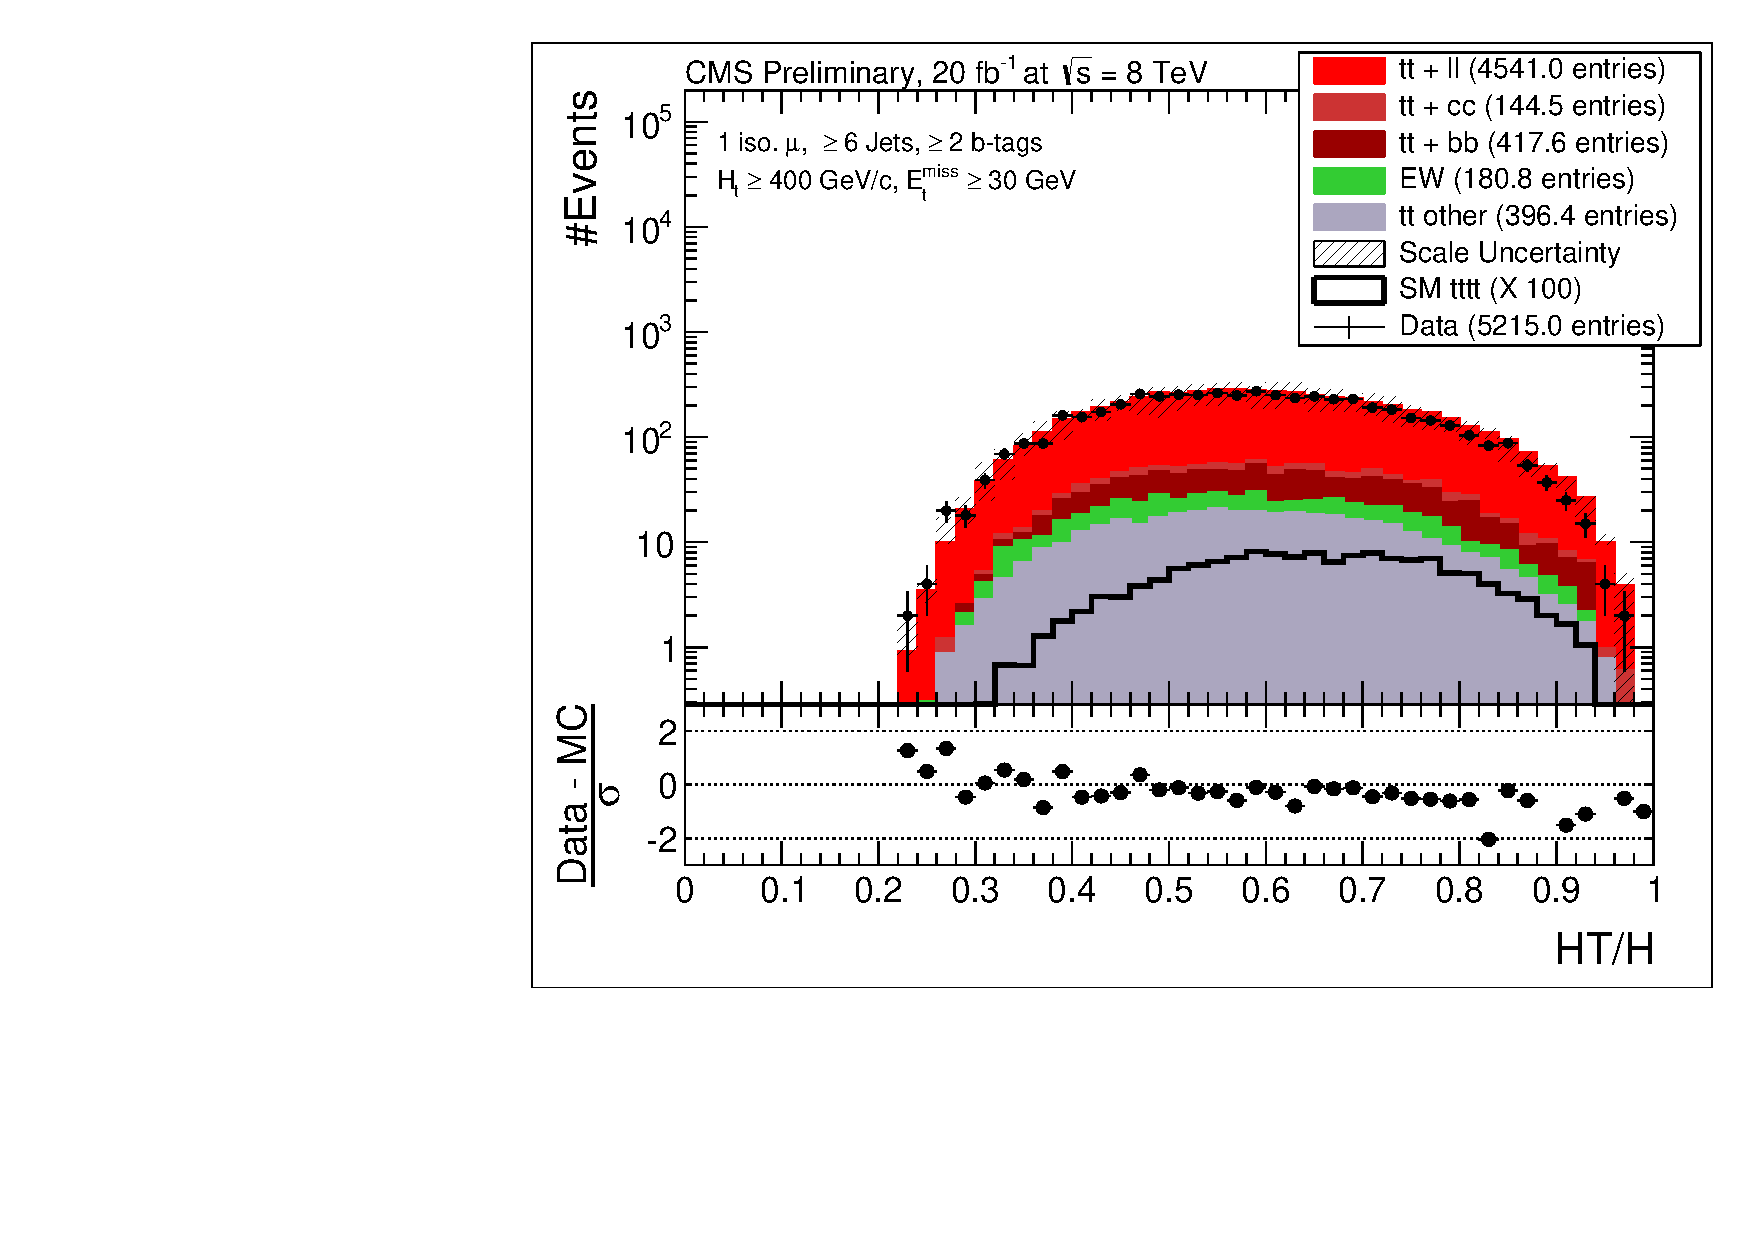
\includegraphics[width=0.49\textwidth]{images/Run1/HTH_StackLogY_Mu.pdf}
    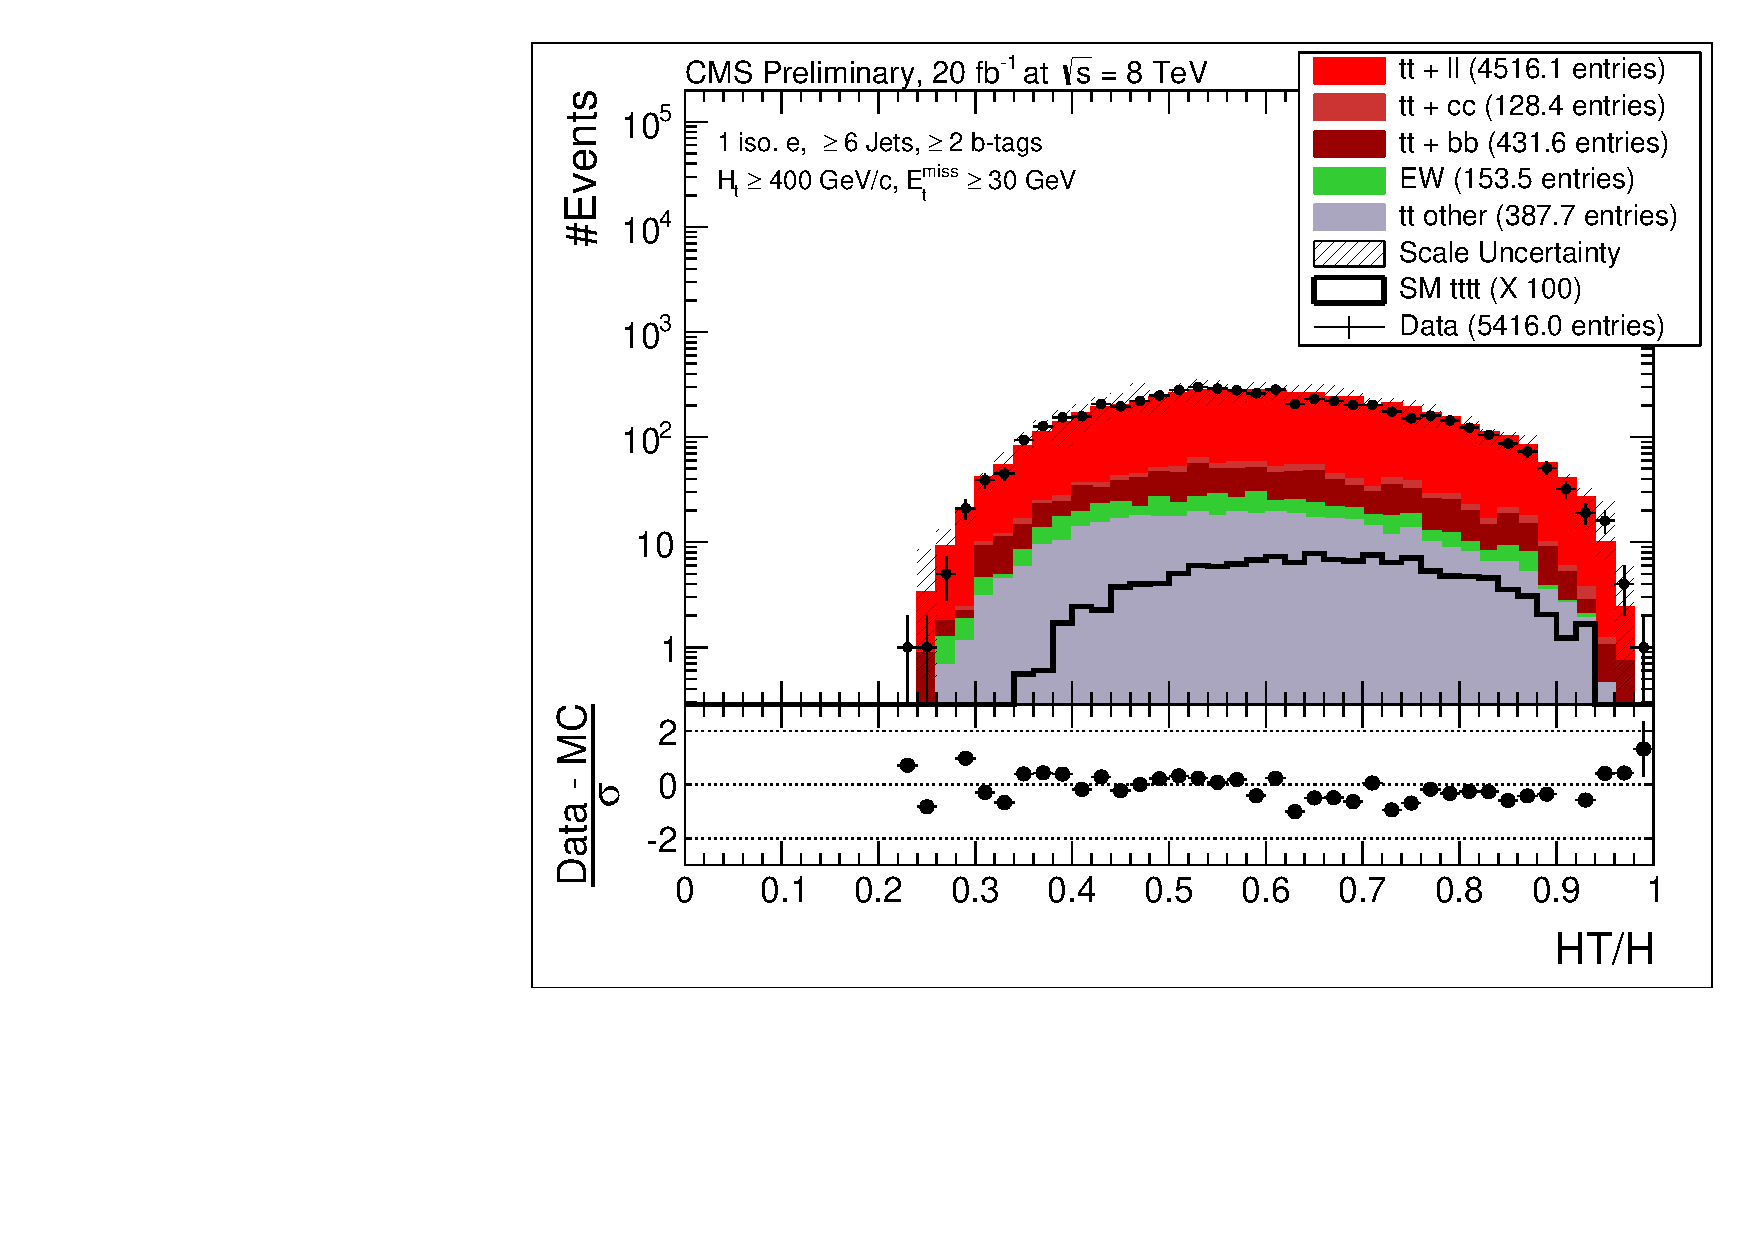
\includegraphics[width=0.49\textwidth]{images/Run1/HTH_StackLogY_e.pdf}
    \caption{Centrality for $\mu$ + jets (right) and e + jets (left).}
    \label{fig:centrality}
\end{figure}

\begin{figure}[!ht]
    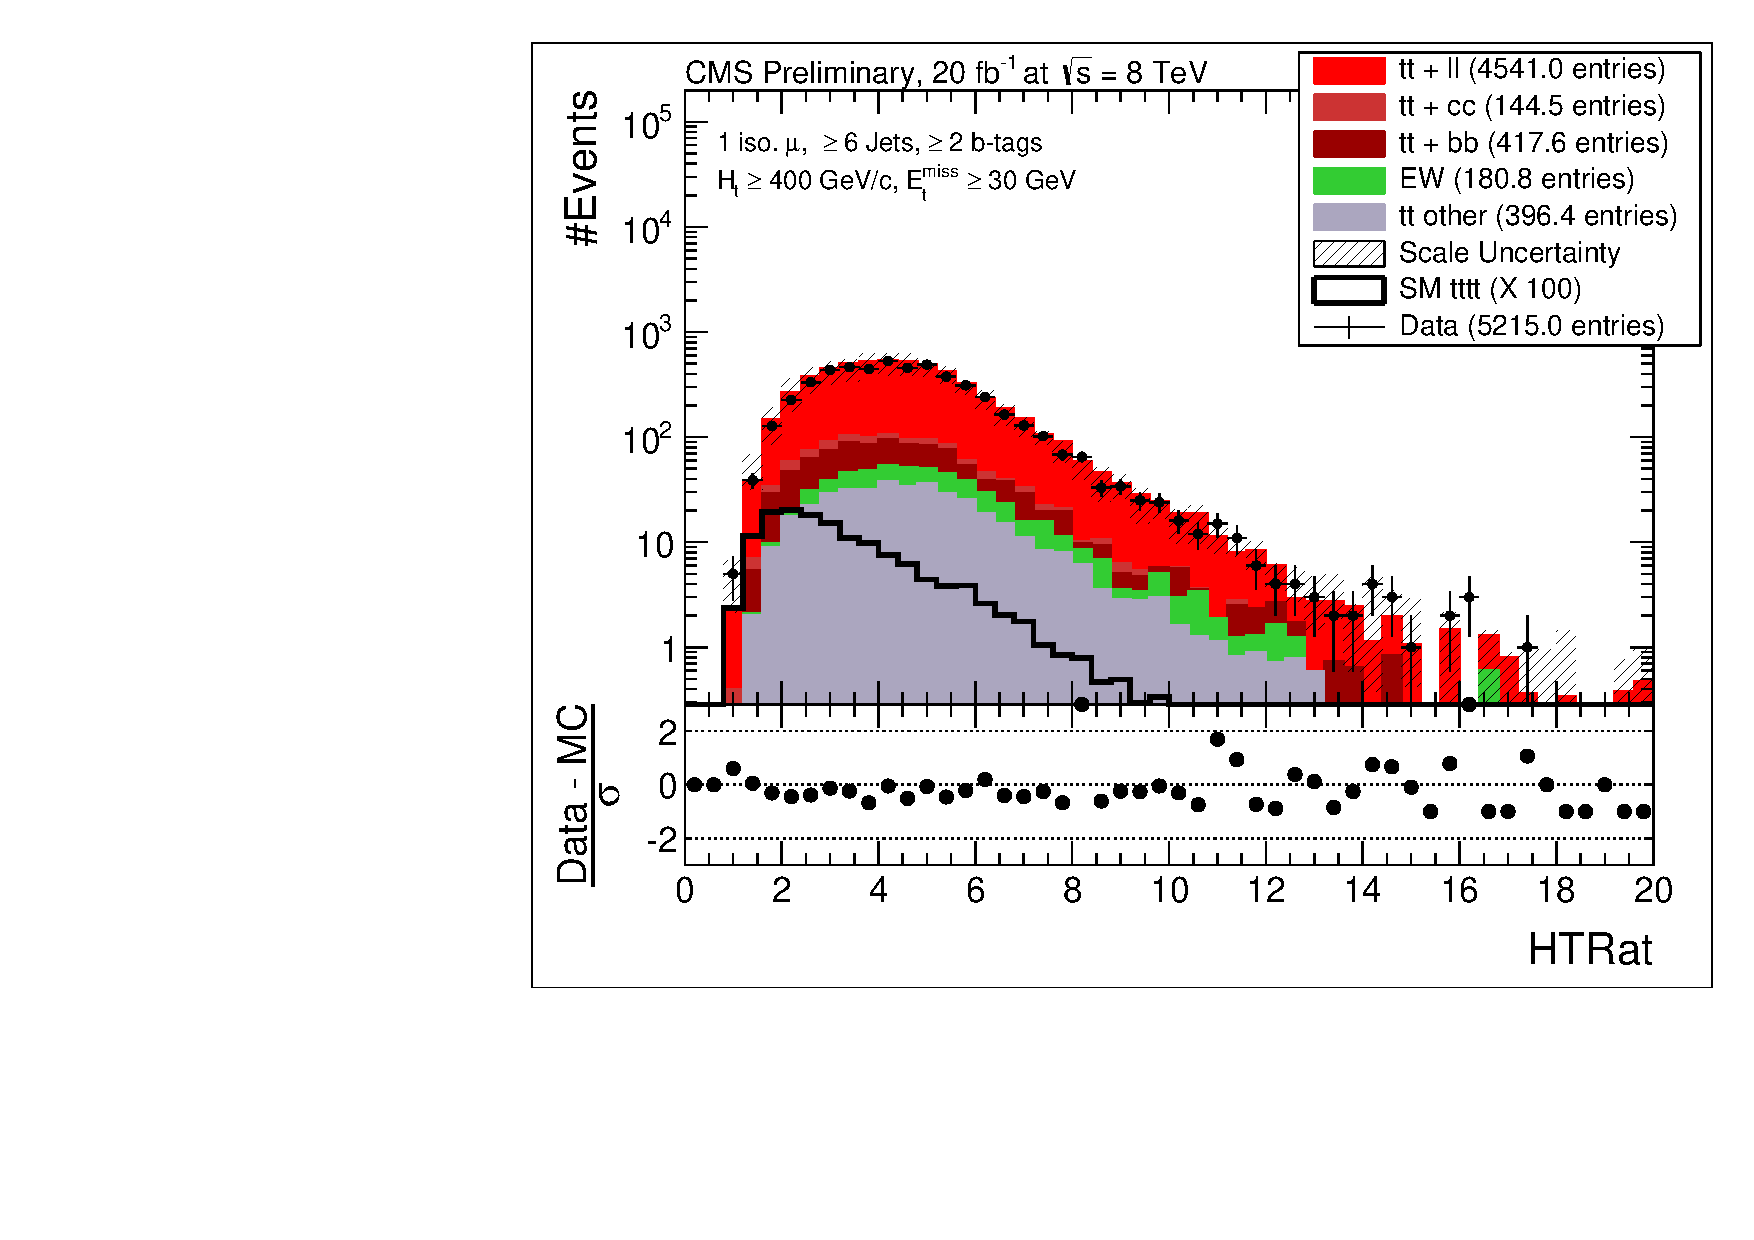
\includegraphics[width=0.49\textwidth]{images/Run1/HTRat_StackLogY_Mu.pdf}
    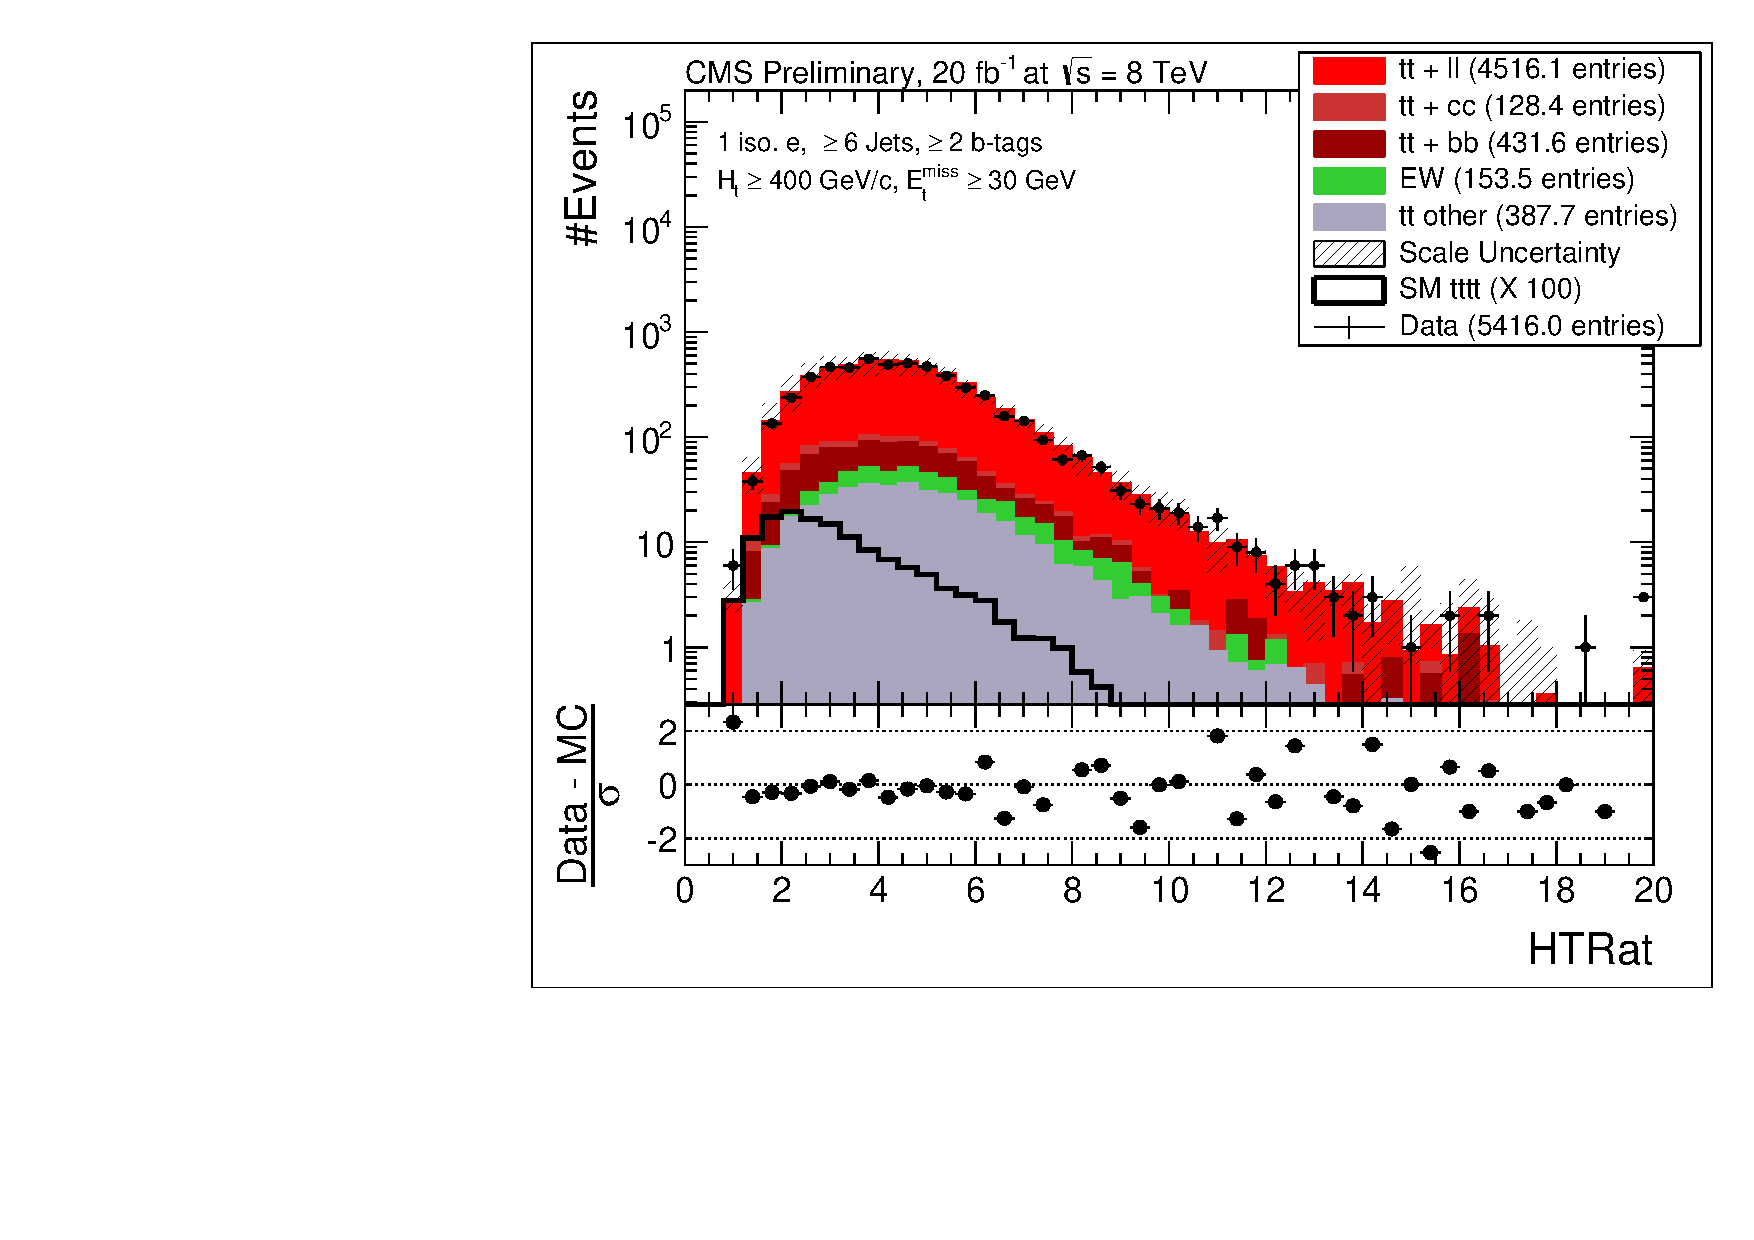
\includegraphics[width=0.49\textwidth]{images/Run1/HTRat_StackLogY_e.pdf}
    \caption{\HTrat for $\mu$ + jets (right) and e + jets (left).}
    \label{fig:HTrat}
\end{figure}

\begin{figure}[!ht]
    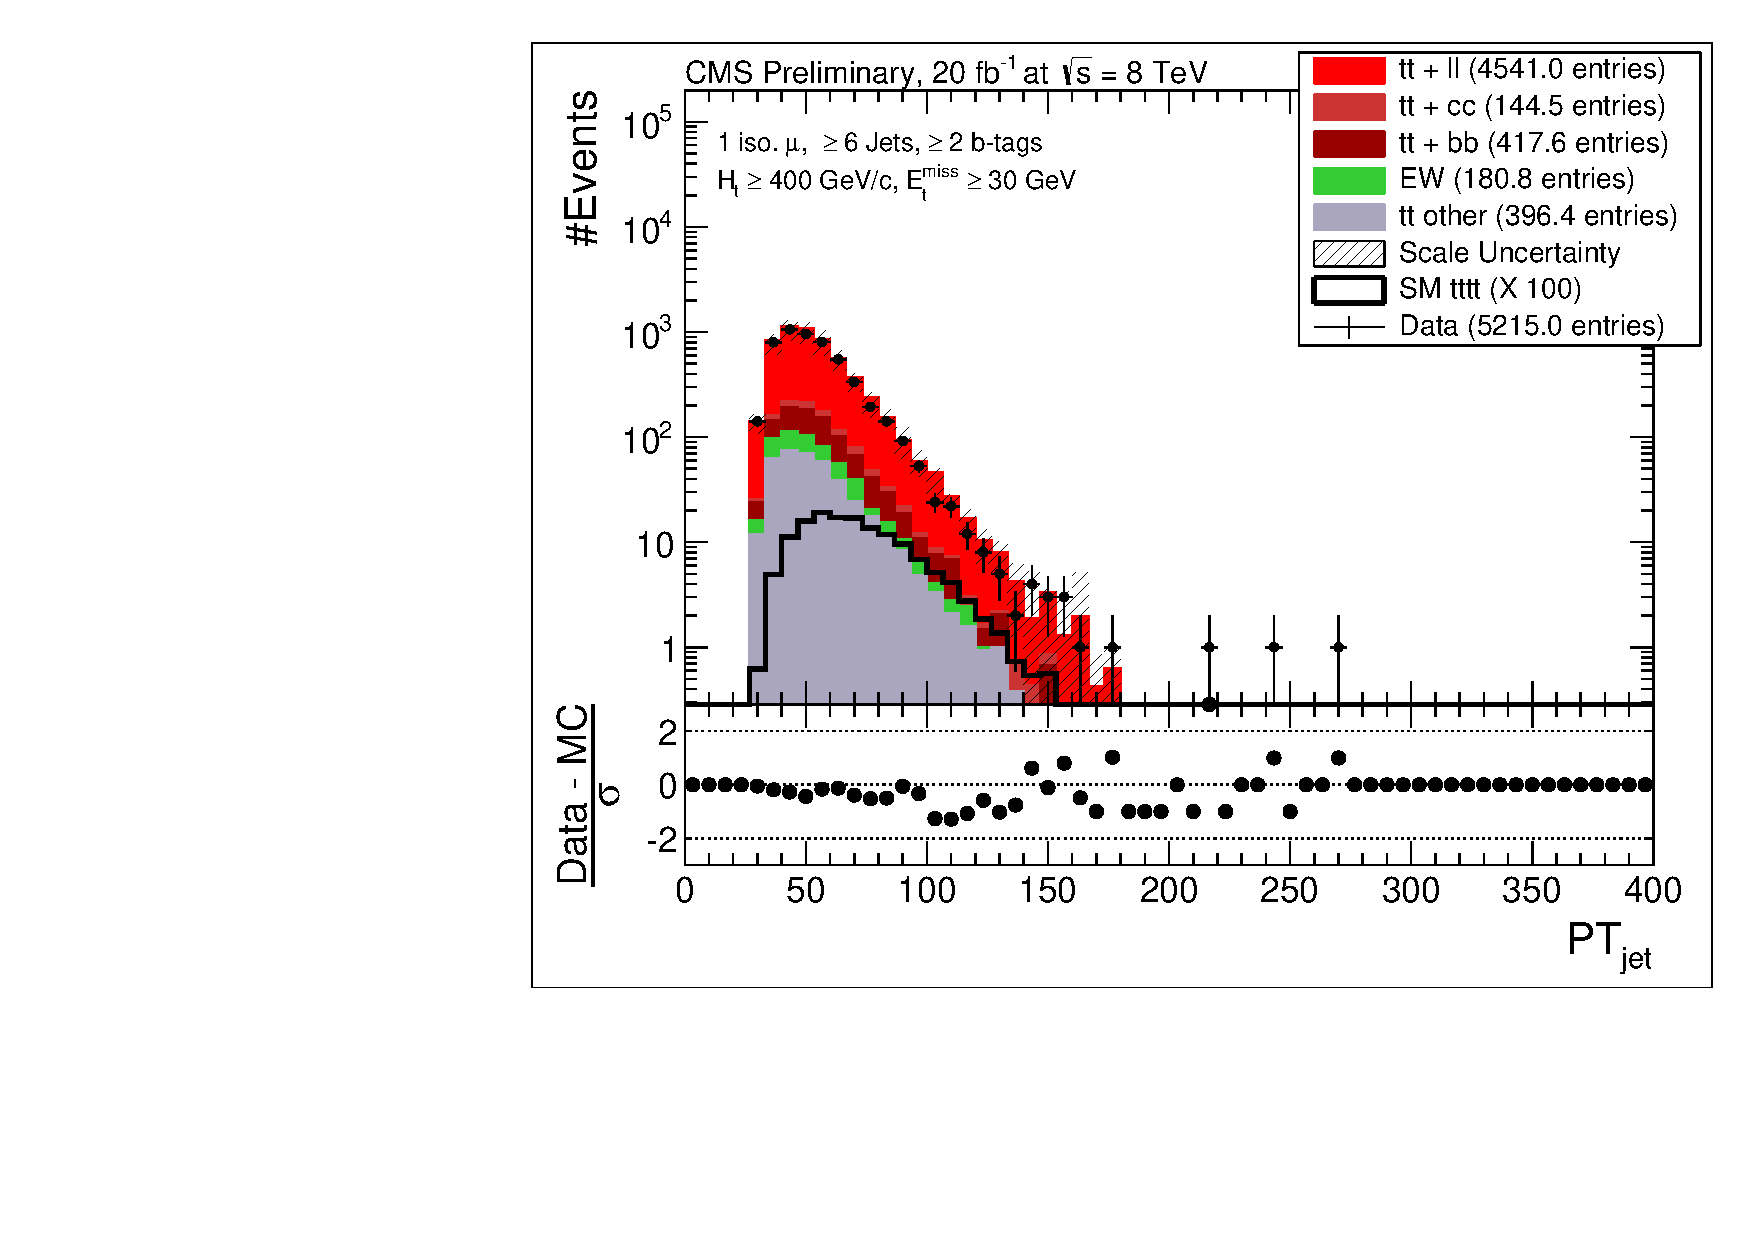
\includegraphics[width=0.49\textwidth]{images/Run1/5thJetPt_StackLogY_Mu.pdf}
    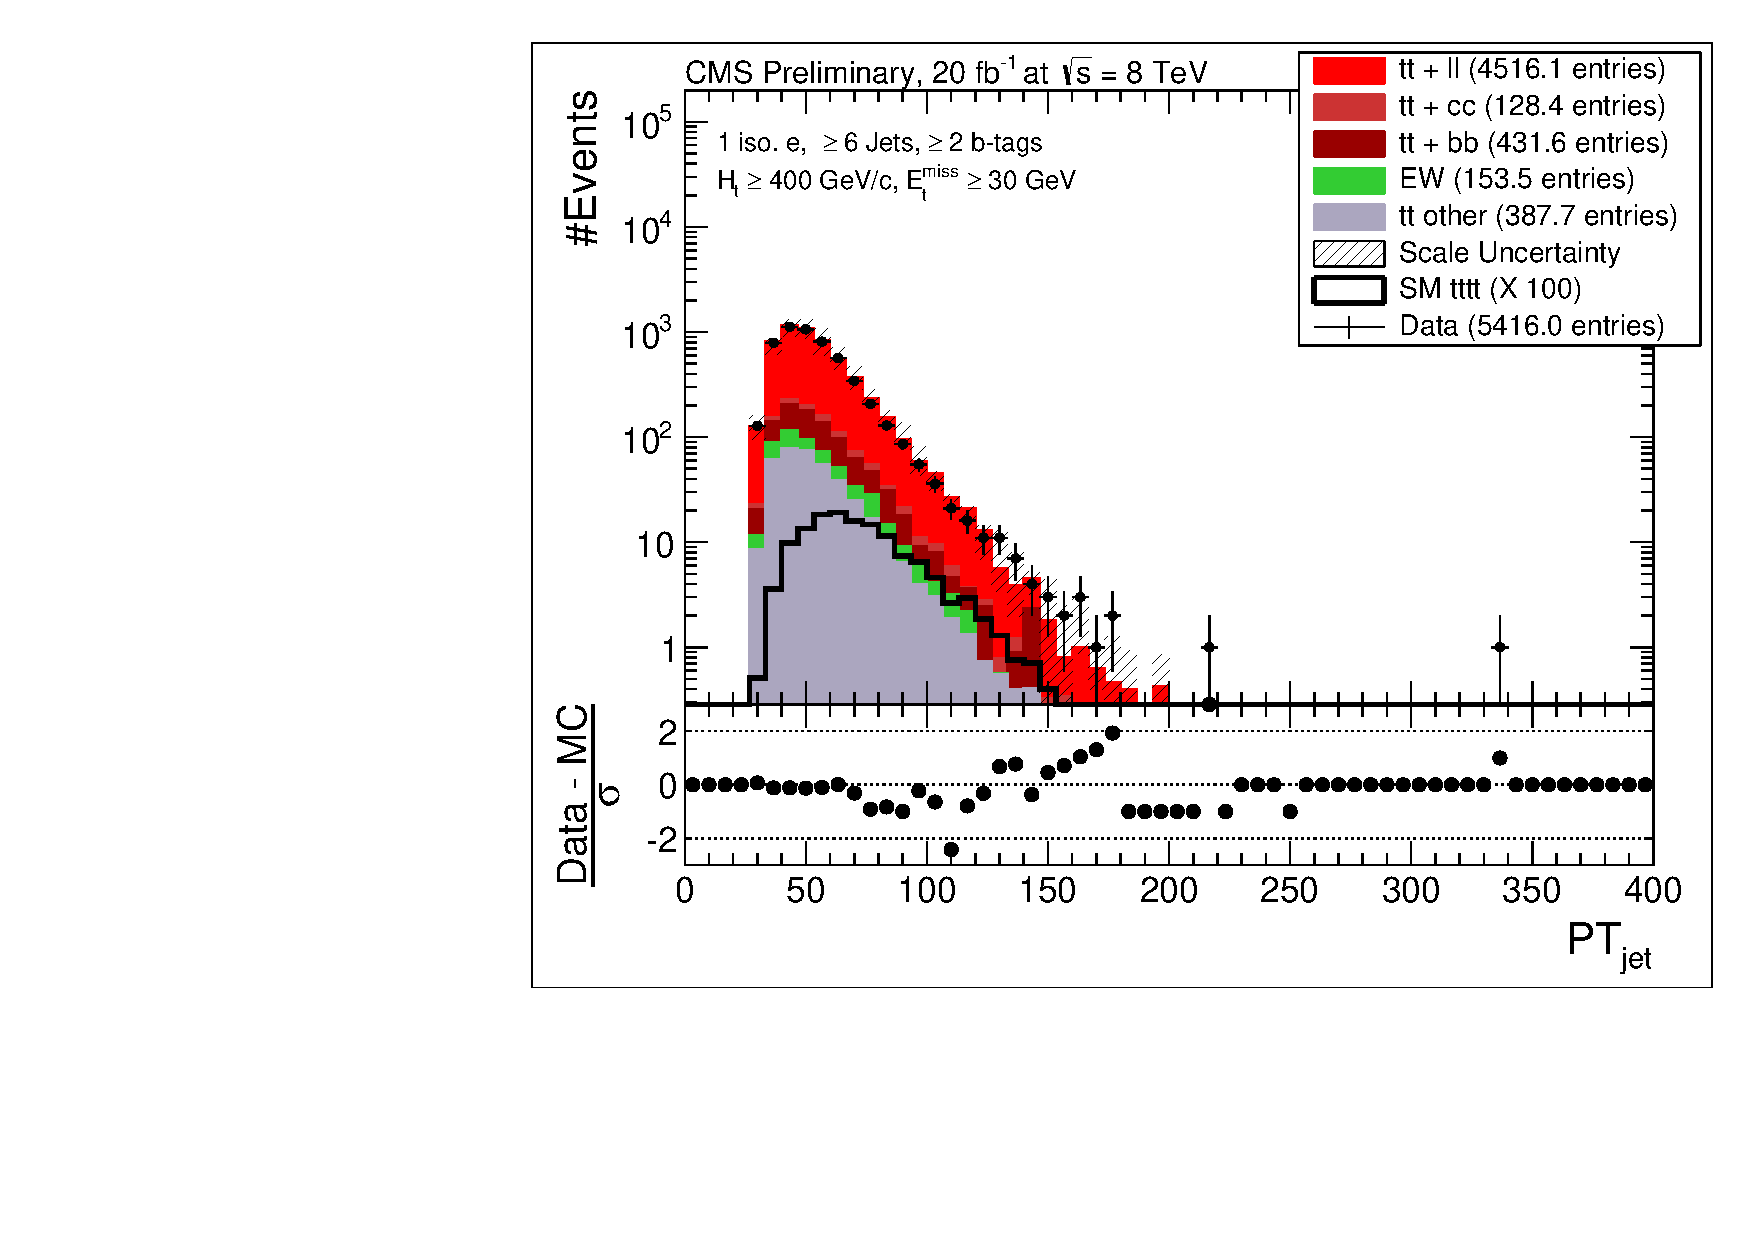
\includegraphics[width=0.49\textwidth]{images/Run1/5thJetPt_StackLogY_e.pdf}
    \caption{5th jet \pt for $\mu$ + jets (right) and e + jets (left).}
    \label{fig:5thjetpt}
\end{figure}

\begin{figure}[!ht]
    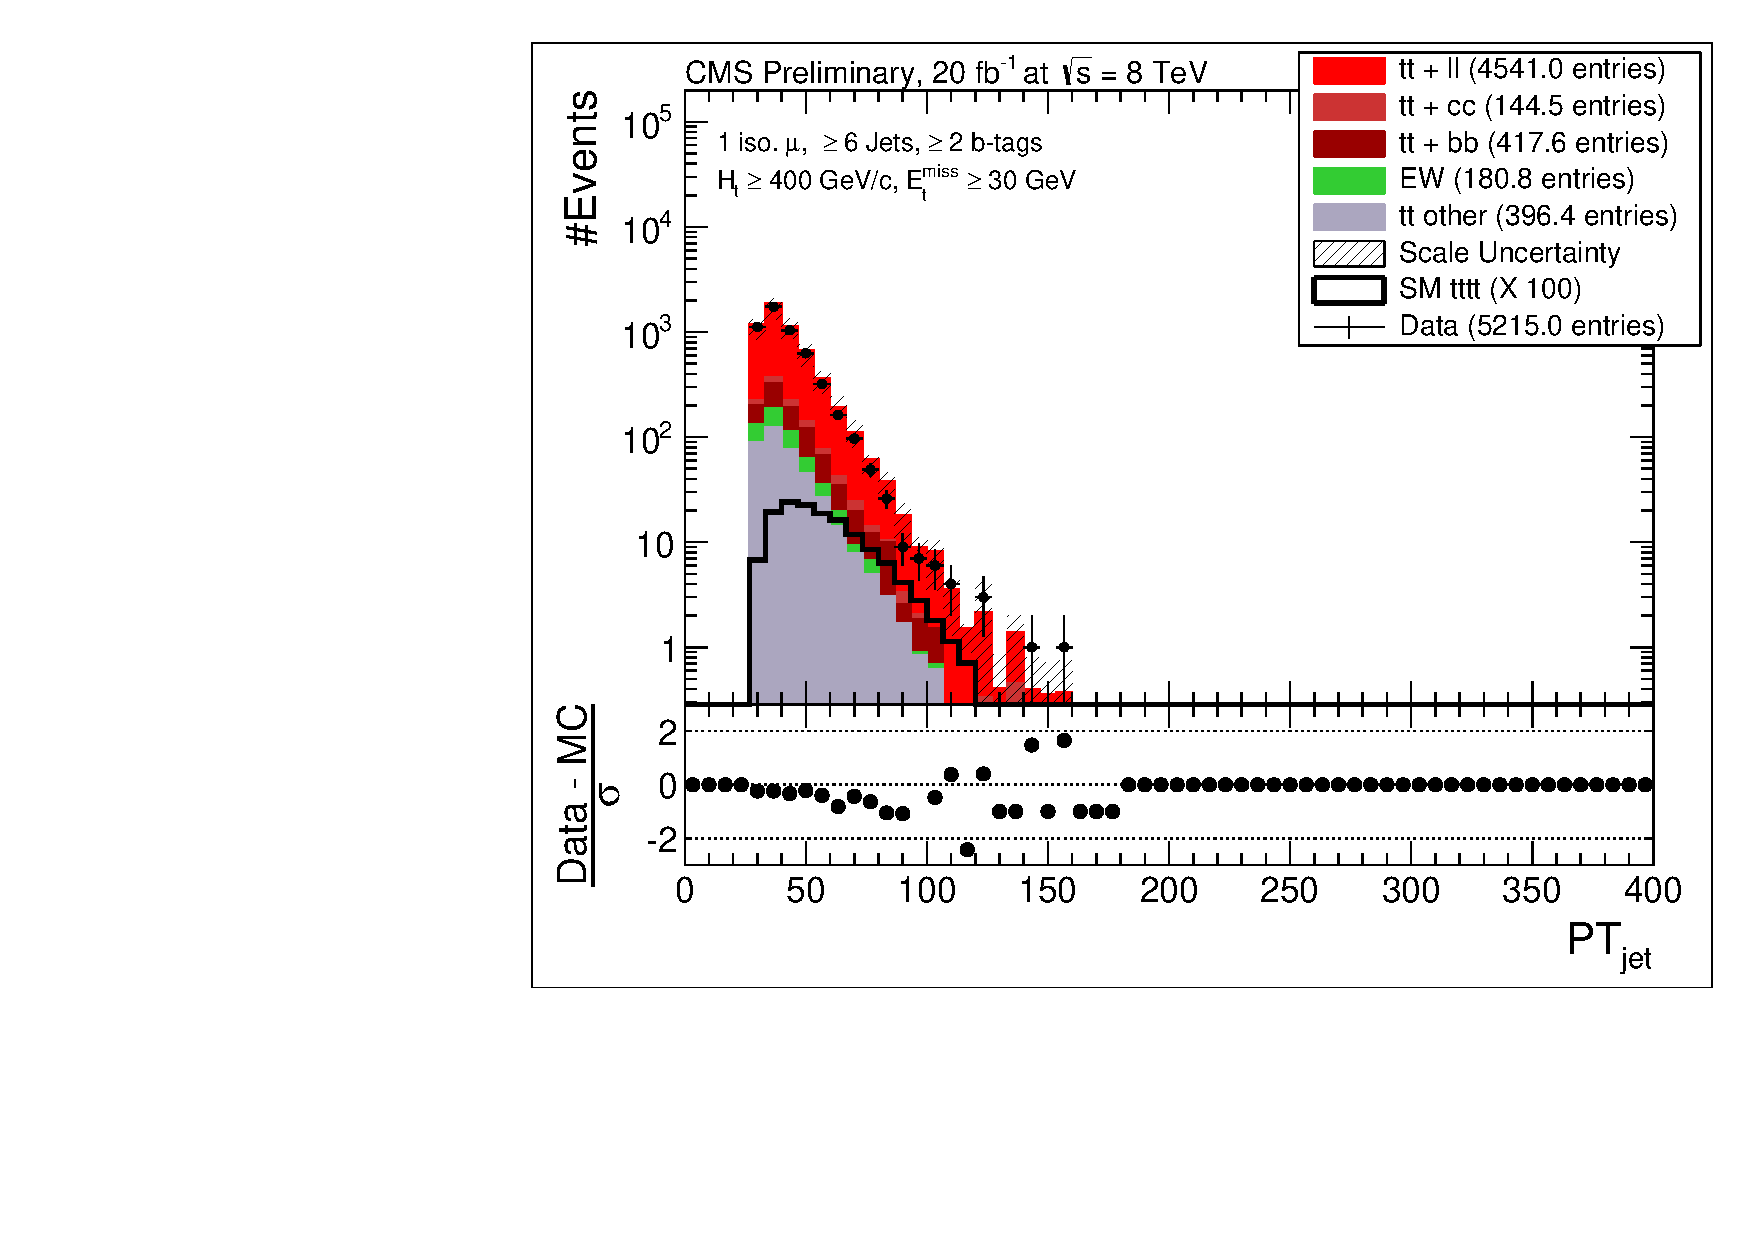
\includegraphics[width=0.49\textwidth]{images/Run1/6thJetPt_StackLogY_Mu.pdf}
    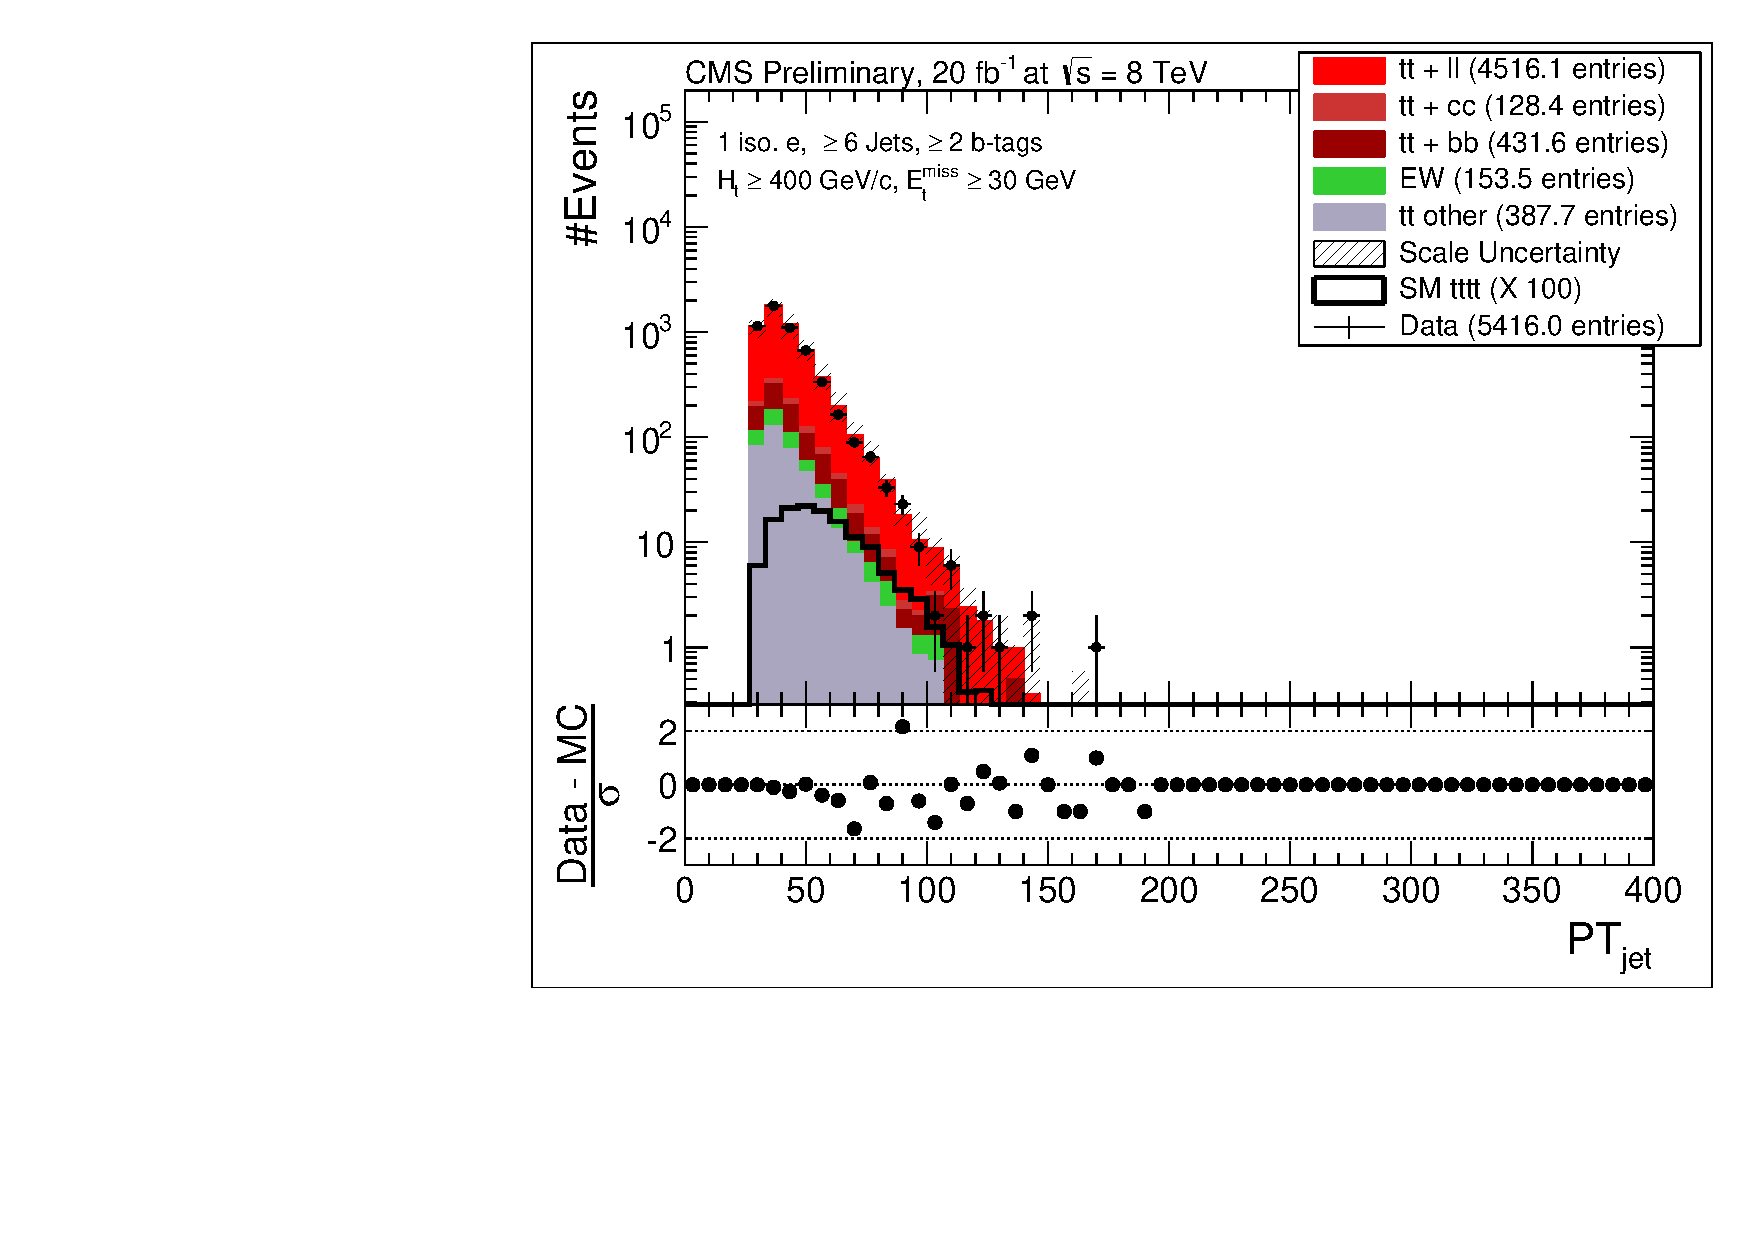
\includegraphics[width=0.49\textwidth]{images/Run1/6thJetPt_StackLogY_e.pdf}
    \caption{6th jet \pt for $\mu$ + jets (right) and e + jets (left).}
    \label{fig:6thjetpt}
\end{figure}

\subsection{Event-level BDT}
% All of the variables described in Sections~\ref{sec:topContent},~\ref{sec:bottomContent} \&~\ref{sec:eventActivity} are used in a BDT, known as the event-level BDT. It is necessary to use 
A sample of events which were not used to train the kinematic reconstruction of top quarks are used to train the event-level BDT so that an orthogonal training sample can be provided. 
% An additional set of events are used to test the performance of the BDT. 
The output distribution of the BDT discriminator can be seen in Fig.~\ref{fig:BDT}. Again, there is good agreement between the data and simulation and it can be seen that there is an improved separation between the background distributions and the \tttt distribution compared to the input variables to the BDT.
% \fxnote{Numbers of events for training?}

\begin{figure}[!ht]
    \includegraphics[width=0.49\textwidth]{images/Run1/MVA_Mu.pdf}
    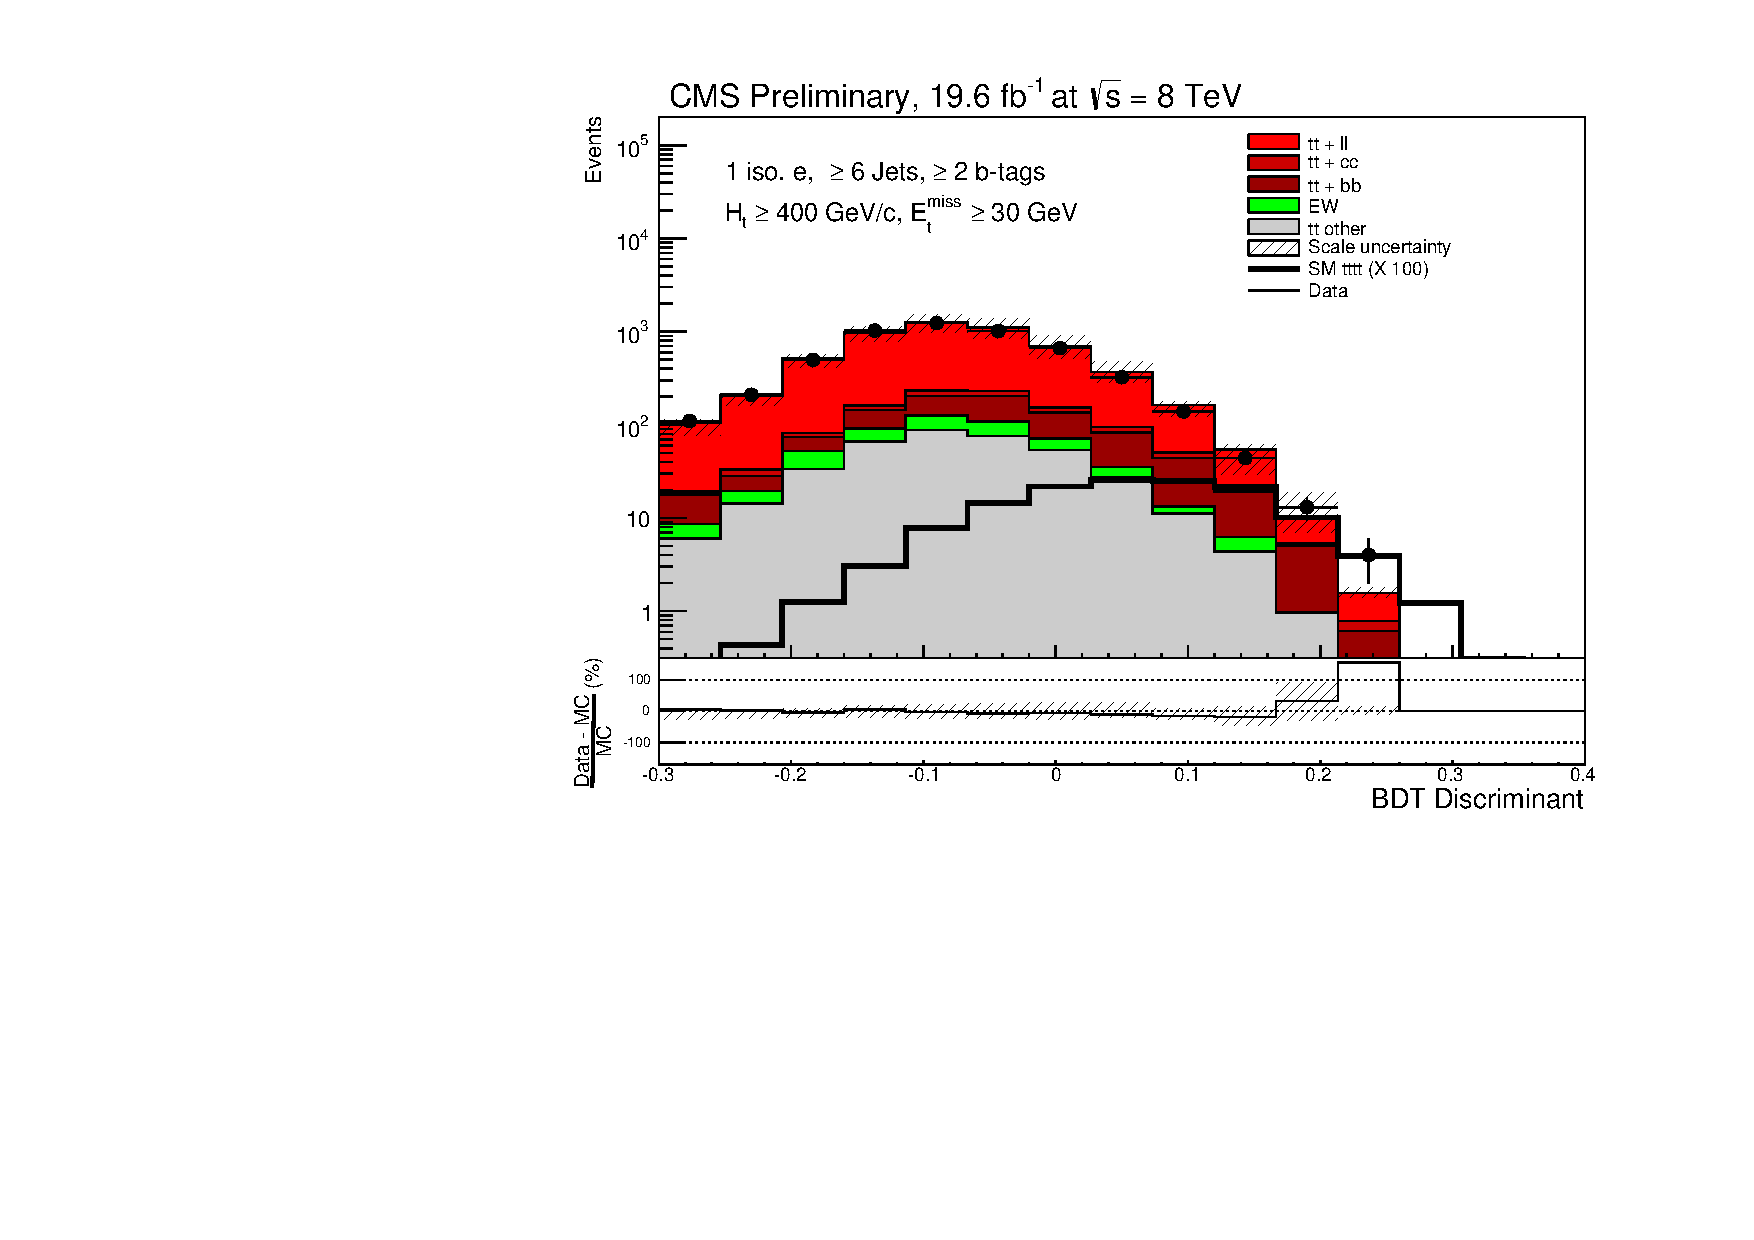
\includegraphics[width=0.49\textwidth]{images/Run1/MVA_e.pdf}
    \caption{BDT discriminator variable in data and simulation for $\mu$ + jets (right) and e + jets (left).}
    \label{fig:BDT}
\end{figure}

\section{Systematic uncertainties}
\label{sec:uncertainties8}
% There are two categories of systematic uncertainties; (i) Uncertainties which affect the normalisation of the distributions which are applied to signal and background and (ii) uncertainties which affect the shape of the distributions which are applied to the dominant background, in this case \ttbar. 

All systematic uncertainties are described in section~\ref{sec:uncertainties} and some further details about them are given below.

% \subsection{Normalisation uncertainties}
% %The normalisation uncertainties will only affect the uncertainty on the expected limit rather than the limit itself when it is used in the template fit and limit setting procedure described in Section~\ref{sec:limit}.
% Normalisation uncertainties include the following:
\begin{itemize}
\item \textbf{Luminosity}\\
The CMS Luminosity Group gave a recommendation of 2.6$\%$ uncertainty on the luminosity~\cite{CMS-PAS-LUM-12-001}.
\item \textbf{Monte Carlo cross sections}\\
As \ttbar is the main background to \tttt, the uncertainty on its MC cross-section is expected to be dominant over the other background processes. The uncertainty on \ttbar is ${}^{+2.5\%}_{-3.4\%} \left( \textrm{renormalisation and factorisation scale} \right)$ and ${}^{+2.5\%}_{-2.6\%} \left( \textrm{PDF} \right)$~\cite{PhysRevLett.110.252004}. The MC cross section uncertainties for the other background processes are modelled by assigning a $4\%$ uncertainty and a $10\%$ uncertainty is assigned to the signal process.
\item \textbf{Factorisation and renormalisation scales}\\
The alternative \ttbar samples with ME and PS scale (u) varied by 2u, 1/2u were used as the alternative shapes.
\item \textbf{Matching threshold}\\
The alternative \ttbar samples with the matching threshold changed between 20~GeV and 40~GeV were used as the alternative shapes.
\item \textbf{JES}\\
The JES uncertainty is derived by varying the JES by $\pm1\sigma$.
\item \textbf{JER}\\
The JER uncertainty is derived by varying the smearing by $\pm1\sigma$.
\item \textbf{b tagging}\\
The b tagging uncertainty is quantified by varying the scale factor by $\pm1\sigma$.
\item \textbf{Pile up}\\
The PU systematic uncertainty is found by varying the MinBias cross section by $\pm5\%$.
\item \textbf{\heavyflavourone / \heavyflavourtwo modelling}
The uncertainty on the measurement of \heavyflavourone / \heavyflavourtwo by CMS~\cite{Khachatryan2015132} is $\pm 0.4 \left( \textrm{stat.} \right) \pm 0.5 \left(\textrm{sys.} \right)$. Alternative event weights are derived for \heavyflavourone / \heavyflavourtwo which are used to provide the alternative systematic up and down templates.
 \end{itemize}
 
% The analysis procedure is repeated with \ttbar samples which have the respective quantity varied by $\pm 1 \sigma$ in order the produce new BDT templates with a deviated shape However, in the case of the matching threshold, the alternative shapes are produced by varying the matching threshold up to 40 GeV and down to 20 GeV.

\section{Template fit and upper limit}
\label{sec:limit}

An upper limit was calculated on the signal strength, $\sigmatttt~/~\sigmattttSM$ , as no excess was observed in the data. Firstly, a template fit of the BDT distributions is made using the Combine Tool~\cite{CMS-NOTE-2011-005} which is based on RooStats~\cite{RooStats:2010,Read:2002hq,Junk:1999kv,Cowan:2011js}.
% , where the systematic uncertainties are modelled as nuisance parameters. Shape uncertainties are constrained using gaussian terms with exponential interpolation whereas the normalisation uncertainties are constrained using lognormal terms. For the statistical uncertainties, a lightweight version of the {Beeston and Barlow method~\cite{Conway:2011in} was used. This gives one nuisance parameter for the total MC estimate and a statistical uncertainty on each bin. 
The background processes are grouped into the following templates for the fit: `\ttbar' for semi-leptonic \ttbar, `electroweak' for W $+$ jets and Z $+$ jets, and `\ttbar\textunderscore other' for all other \ttbar processes. Using the \CLS method~\cite{Junk1999435,0954-3899-28-10-313} with the asymptotic approximation, the best fit values of the nuisance parameters can be obtained along with the corresponding limit on $\sigmatttt~/~\sigmattttSM$. The cross section limit, \sigmatttt, can be derived by multiplying $\sigmatttt~/~\sigmattttSM$ by \sigmattttSM $\approx 1.3$.

\subsection{Splitting into \njets categories}
\label{sec:njetcatlimit}
To increase the sensitivity of the analysis, the BDT templates were split into three \njets categories (\njets $= 6$, \njets $= 7 $ \& \njets $\geq 8$) each for the muon and electron channel. The higher \njets categories benefit from better discrimination power between signal and background as \tttt events are likely to have a larger number of jets. The \njets $= 6$ category helps to constrain the main background of \ttbar. A simultaneous fit of these three \njets categories is made for the muon channel, the electron channel and a combination of the two. The limits extracted using the \CLS method are shown in Table~\ref{tab:lims}.


\begin{table}[ht!]
\centering
\begin{tabular}{| l | l | l | p{1cm} |}
 \hline 
 Channel & Exp.  &Obs. \\
   \hline
 $\mu$ + jets & $35.6\pm 18$ & 34 \\
  \hline
$e$ + jets &  $36.1\pm16$  & 36  \\
\hline
 combined & $24.6\pm13$  & 25   \\
\hline
\end{tabular}
\hspace{0.5cm}
\begin{tabular}{| l | l | l | p{1cm} |}
 \hline 
 Channel & Exp. (fb) &Obs. (fb) \\
   \hline
 $\mu$ + jets & $46.3\pm23$ & 44 \\
  \hline
$e$ + jets &  $47.0\pm20$  & 47  \\
\hline
 combined & $32.0\pm17$  & 32   \\
\hline
\end{tabular}
\caption{CLS limits on (\sigmatttt/(\sigmattttSM) (left) and \sigmatttt (right). }
\label{tab:lims}
\end{table}

In comparison, the corresponding limit for a simultaneous fit of the electron and muon channels in inclusive \njets categories was observed to be 63~fb with an expected limit of  $42^{+18}_{-13}$~fb~\cite{CMS-PAS-TOP-13-012}. Therefore, it can be seen that splitting into \njets categories provides a significant improvement in the sensitivity of the analysis.

\section{Systematics studies and tests on analysis\label{studies8}}

\subsection{Signal Injection Test}
\label{sec:signalinjection}
In order to validate the limit-setting method, the following closure test was performed. A range of signal strengths were injected into the data and the limit-setting procedure was repeated as in Section~\ref{sec:limit}. Figure~\ref{fig:SigInjection} shows the BDT discriminator distributions with injected signal strengths of 20fb, 40fb and 60fb. With the increasing signal strength, there is an increase for data in the bins with a higher BDT discriminator values as would be expected for signal events.
\begin{figure}[ht!]
\centering
    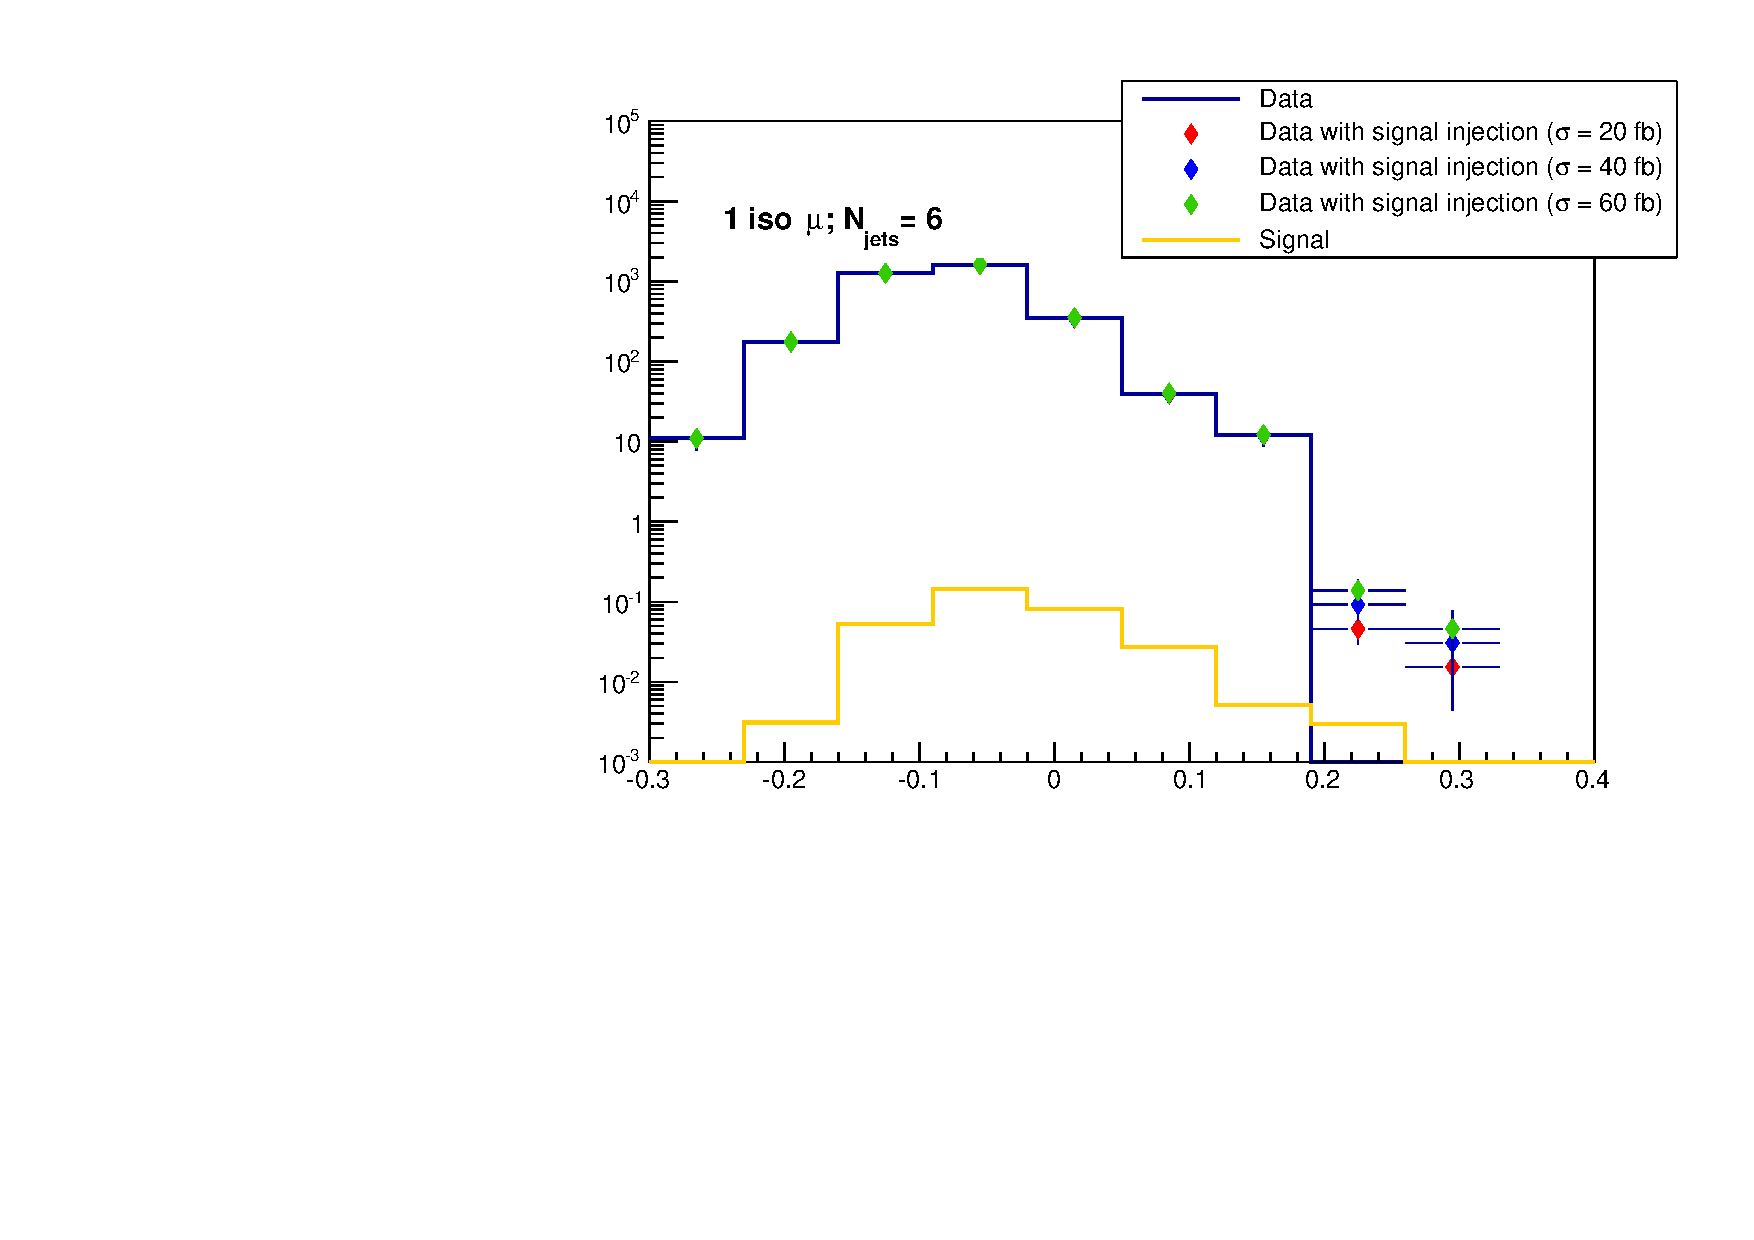
\includegraphics[width=0.49\textwidth]{images/Run1/SignalInjection_Mu_6j.pdf}
     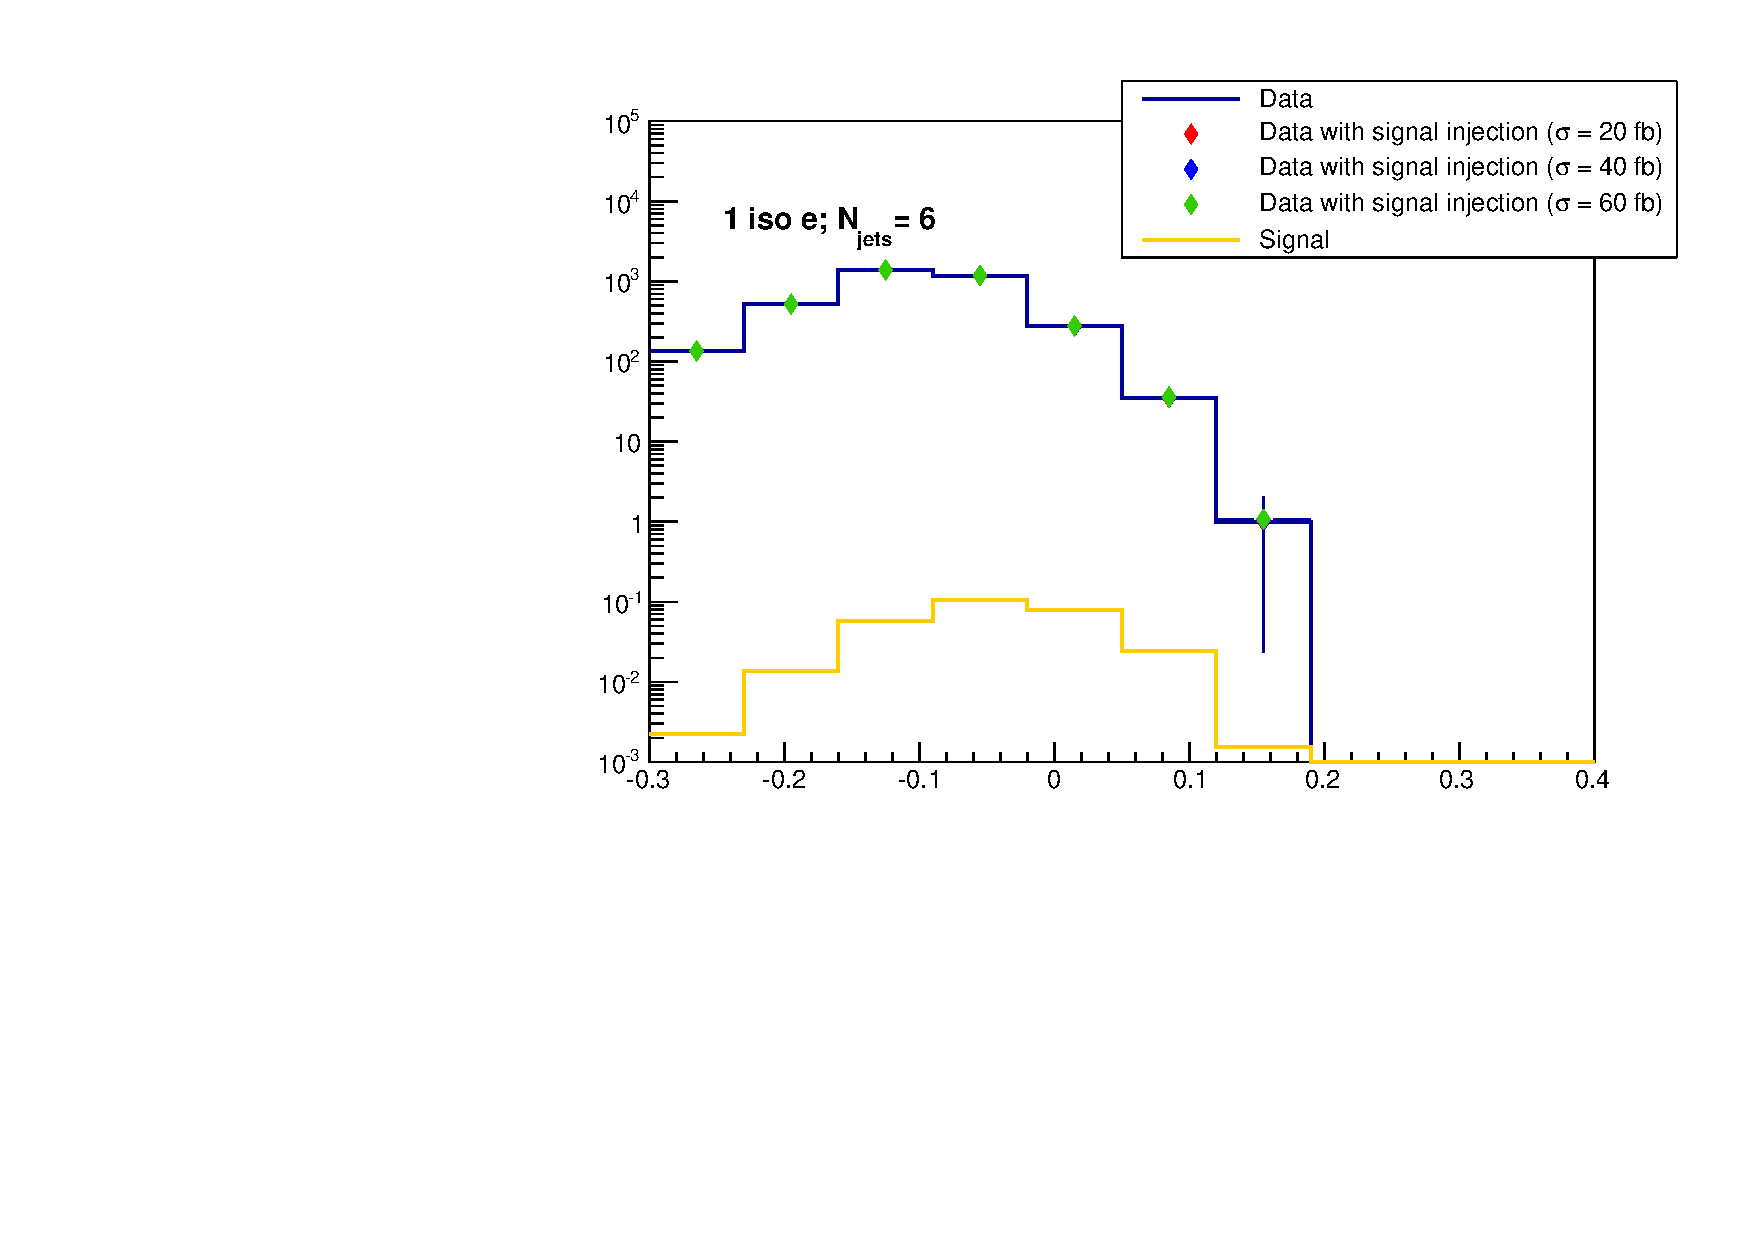
\includegraphics[width=0.49\textwidth]{images/Run1/SignalInjection_El_6j.pdf}
    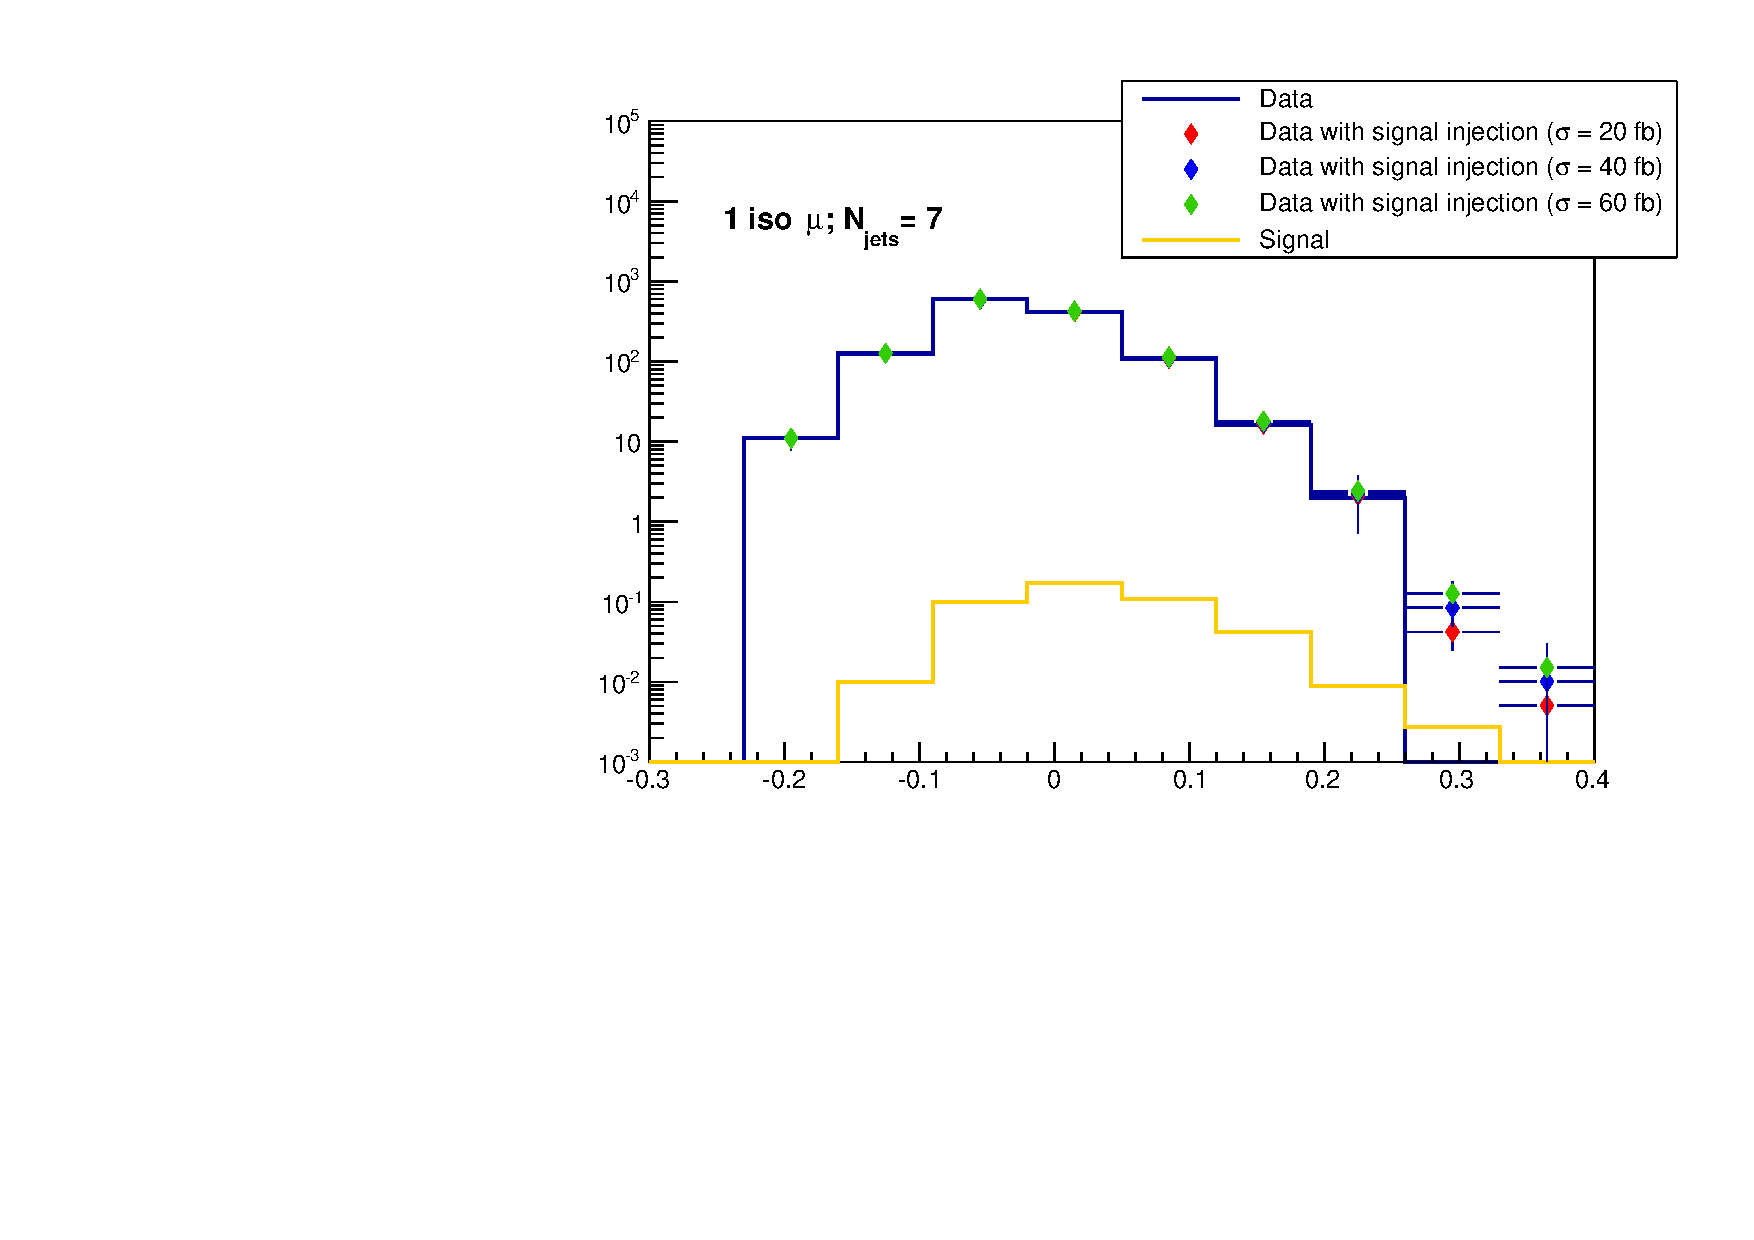
\includegraphics[width=0.49\textwidth]{images/Run1/SignalInjection_Mu_7j.pdf}
     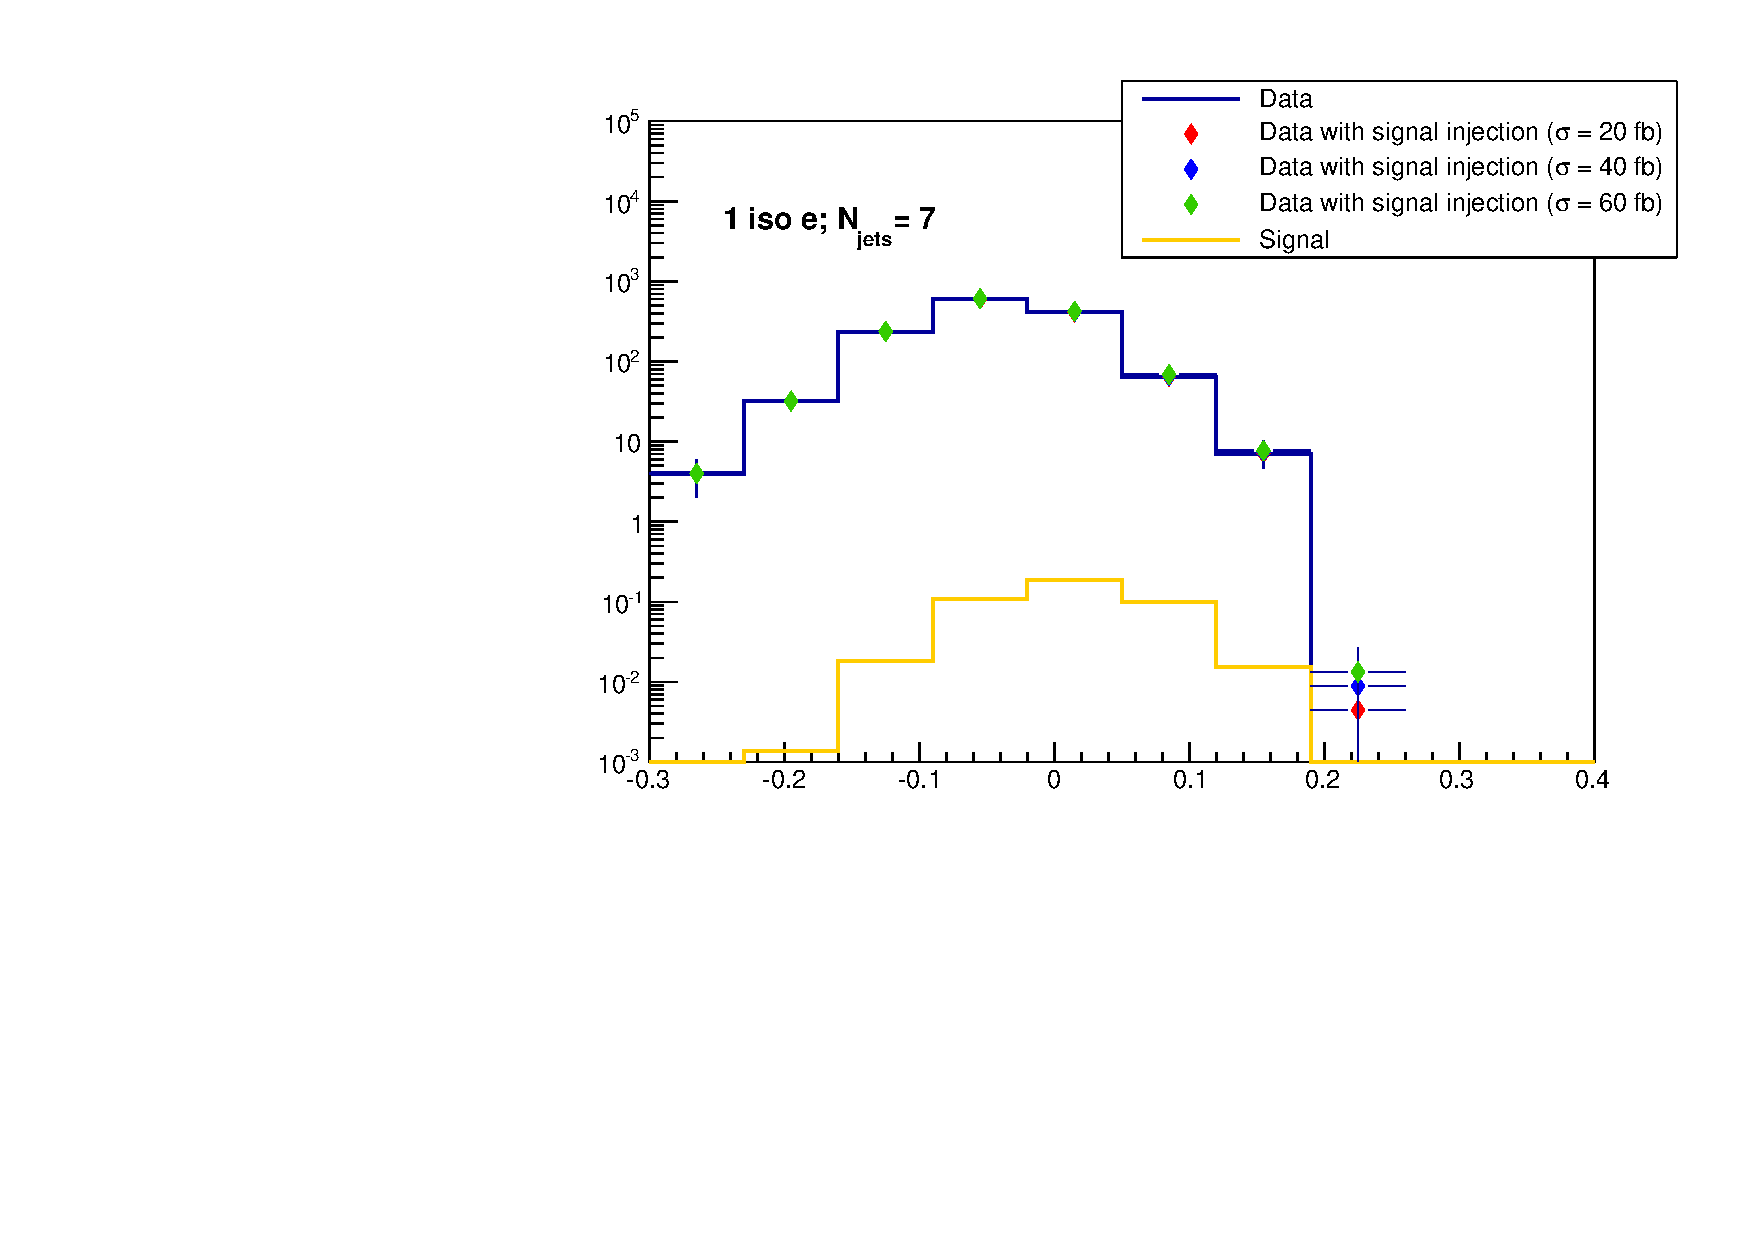
\includegraphics[width=0.49\textwidth]{images/Run1/SignalInjection_El_7j.pdf}
    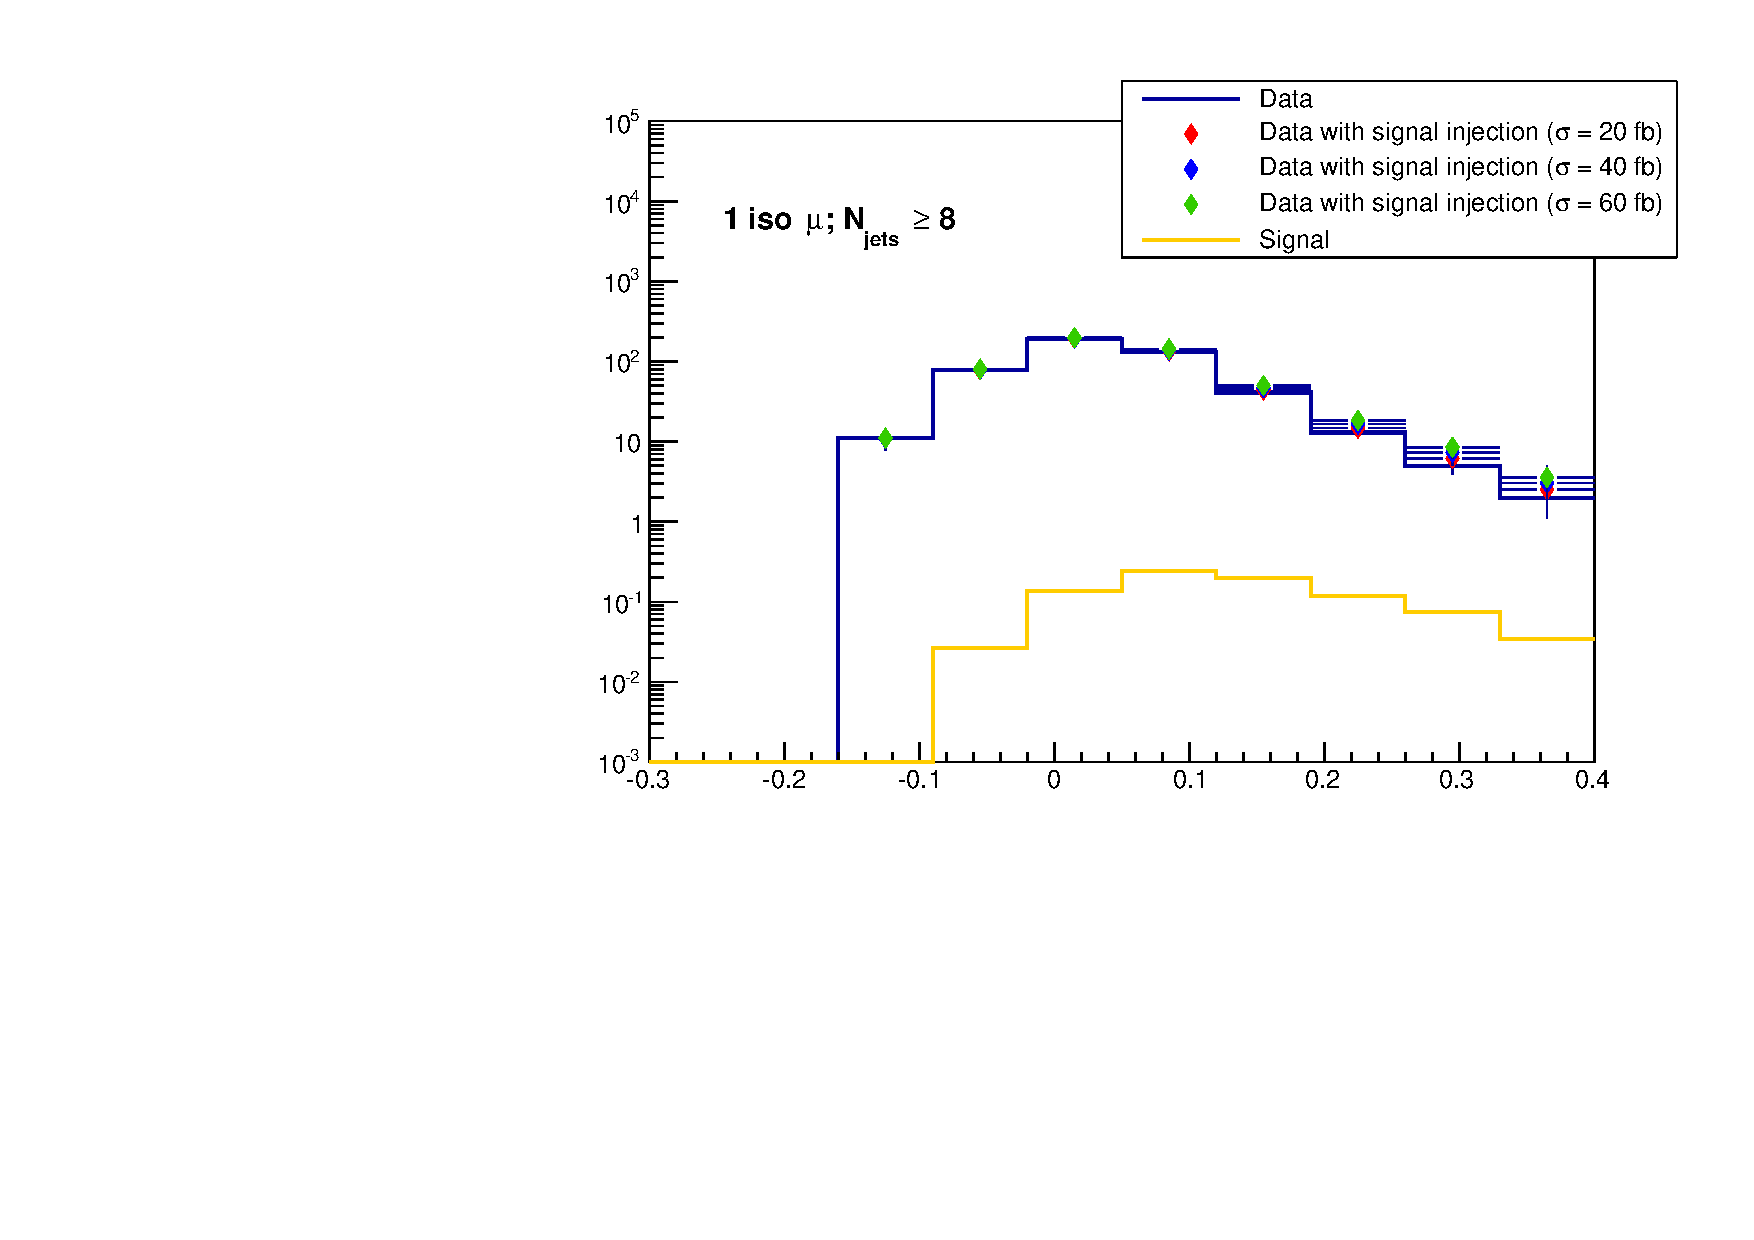
\includegraphics[width=0.49\textwidth]{images/Run1/SignalInjection_Mu_8j.pdf}
     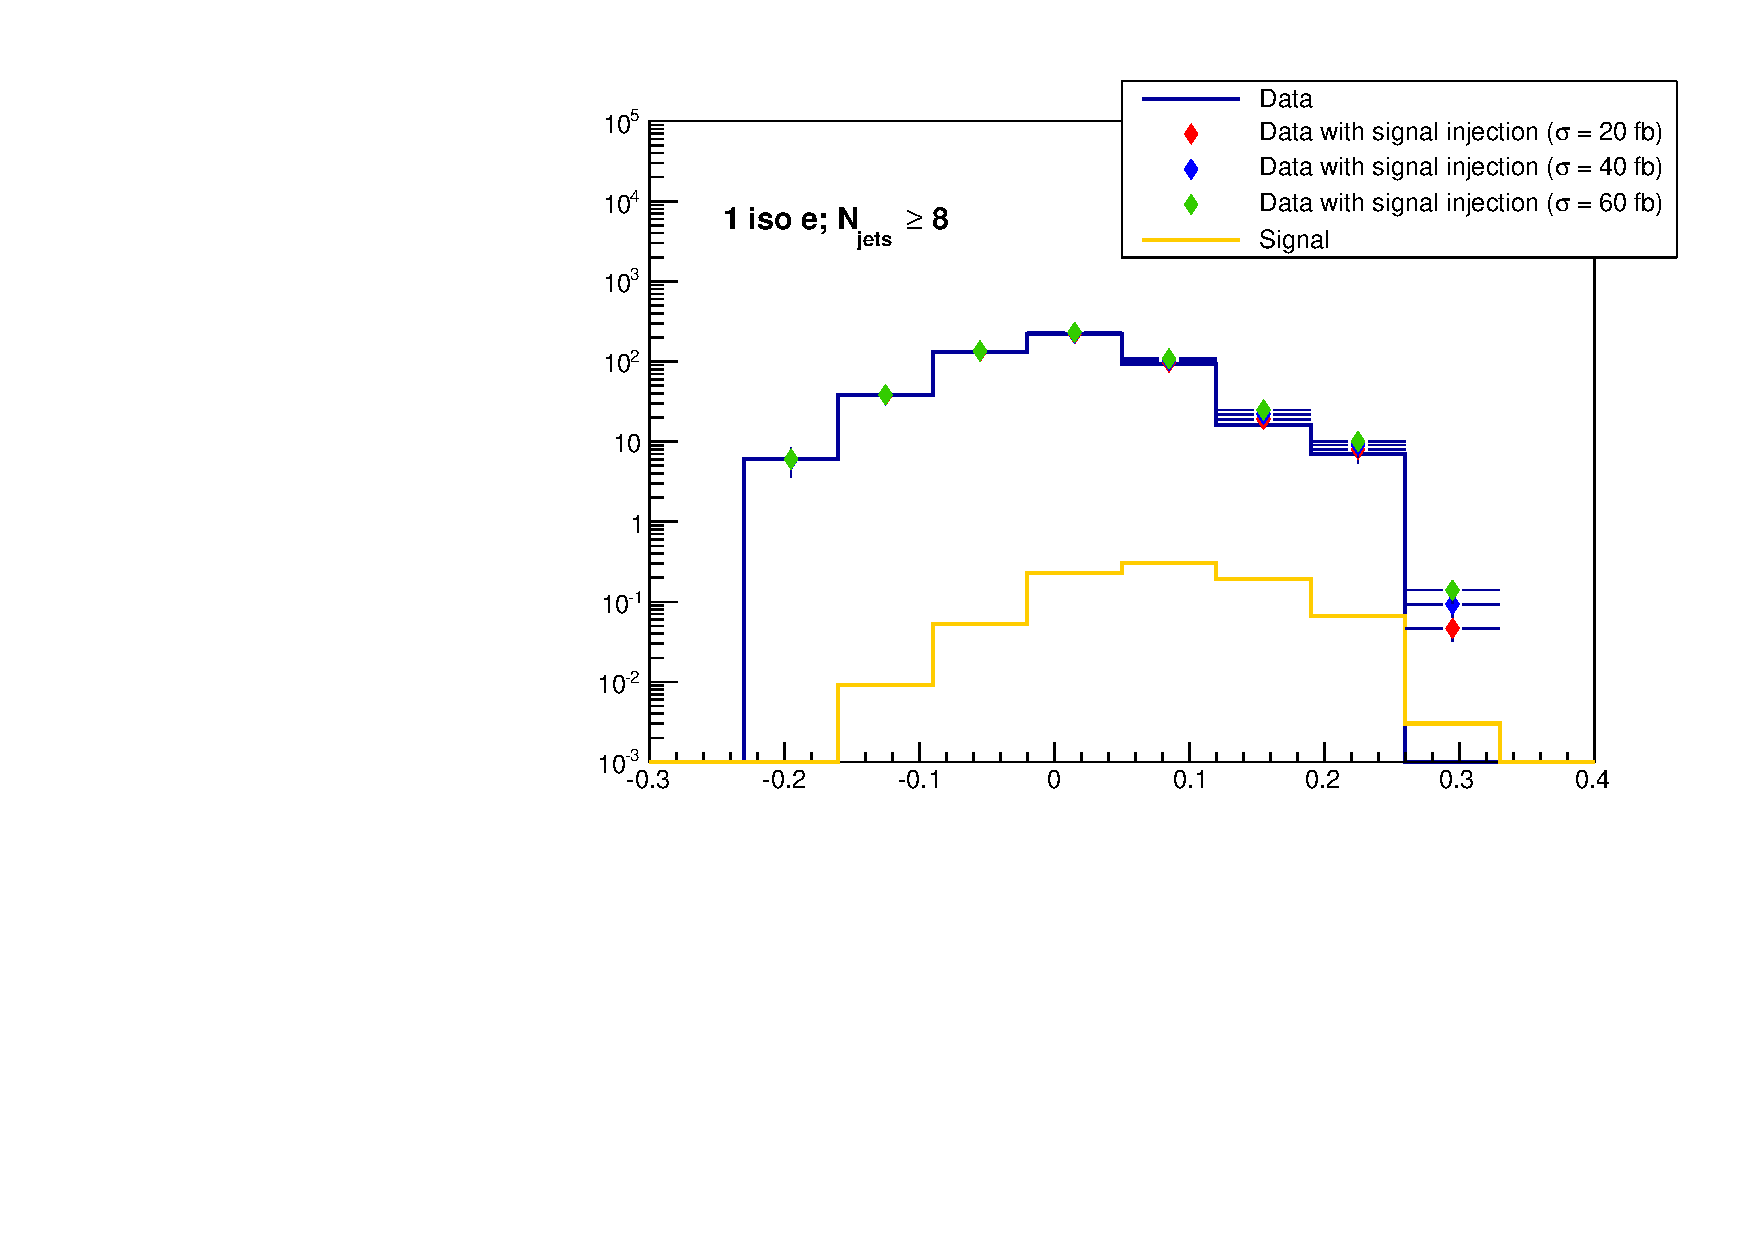
\includegraphics[width=0.49\textwidth]{images/Run1/SignalInjection_El_8j.pdf}          
    \caption{The BDT discriminator distributions of data and the mixtures of data and injected signal are compared for $\mu$ + jets channel $\left( \textrm{left} \right)$ and e + jets channel $\left( \textrm{right} \right)$. }
    \label{fig:SigInjection}
\end{figure}

\begin{figure}[!ht]
\centering
    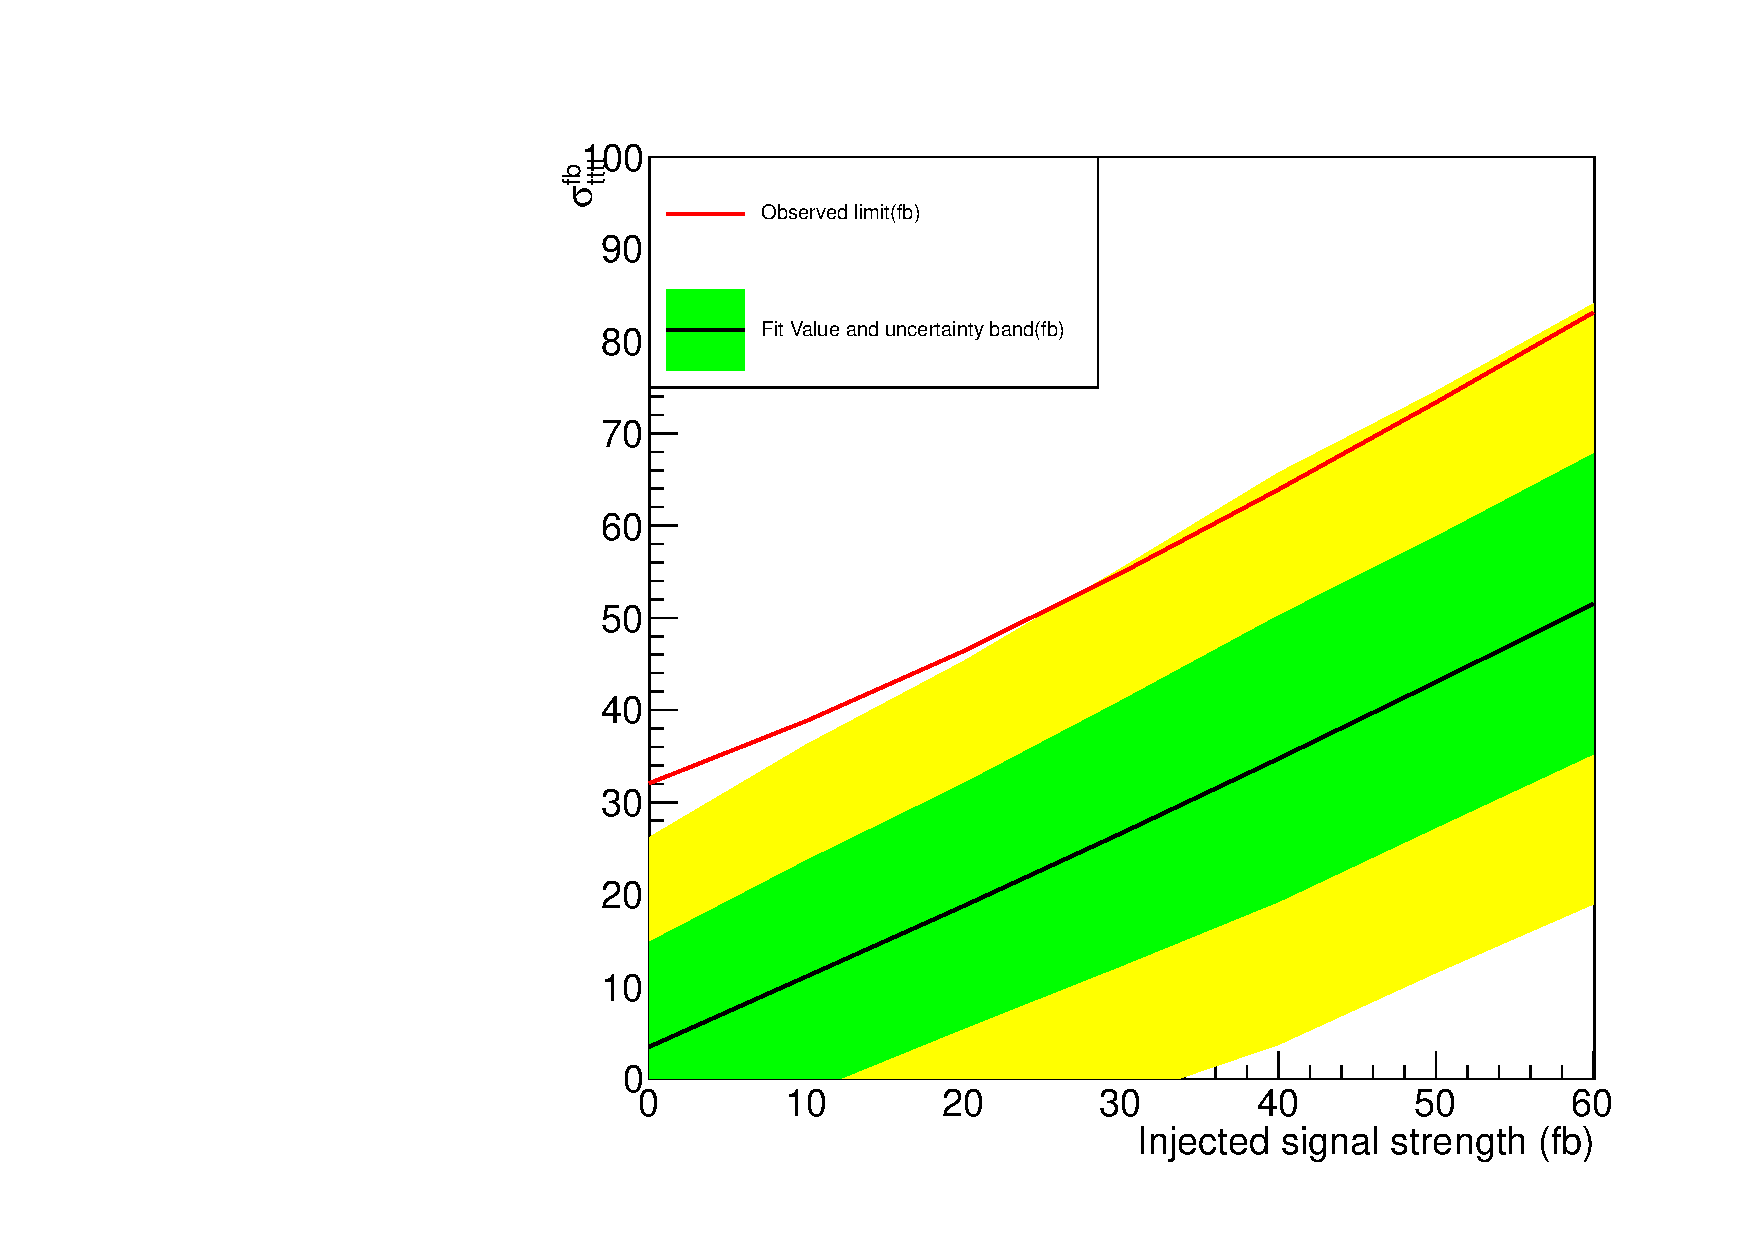
\includegraphics[width=0.6\textwidth]{images/Run1/SignalInjection_JS_Brazil.pdf}
    \caption{Fitted values(fb) and observed(fb) for various injected signal strength(fb).}
    \label{fig:SigInjectionBrazil}
\end{figure}

As can be seen in Fig.~\ref{fig:SigInjectionBrazil}, the fitted value for the signal strength and observed limit increase with increasing injected singal strength as expected. However, there appears to be some bias in the analysis towards selecting background as opposed to signal as can be seen from the gradient of the line, which is $<$1.

% \subsection{Systematics studies}

\subsection{Negligible uncertainties}
\emph{This study was undertaken before the decision was made the split the BDT templates by the \njets categories.}

A few systematatic uncertainties were studied which ultimately had so little impact on the analysis that they were not included in the final result.

In the 2012 CMS differential cross-section \ttbar analysis \cite{CMS:TopPt} the \pt spectrum of top quarks is harder in the \MADGRAPH simulation than it is in data. Scale factors were derived by CMS to compensate for this effect. The analysis was performed with and without the application of the top \pt scale factors and the observed effect was negligible, as seen in Fig.~\ref{fig:studies8}, and hence these scale factors were not applied for the final result.\\
The uncertainty on the parton distribution functions (PDFs) are a potential source of systematic uncertainty. The method used by CMS to model this effect is given here~\cite{ref:PDFUnc2}. The BDT distributions which correspond to the maximal downward and upward fluctuation due to the uncertainty on the PDFs have a very small effect on the shape of the BDT, as seen in Fig.~\ref{fig:studies8}, and are not considered further.\\
The uncertainty due to the choice of \PYTHIA tune used in the hadronisation of \ttbar events is considered. The nominal tune used is the $Z2^{*}$ tune which is compared to the alternative $P11$ tune. Again, there is a very small effect on the shape of the BDT, as seen in Fig.~\ref{fig:studies8}, so this uncertainty is not included in the final fit.

\begin{figure}[ht!]
\centering
    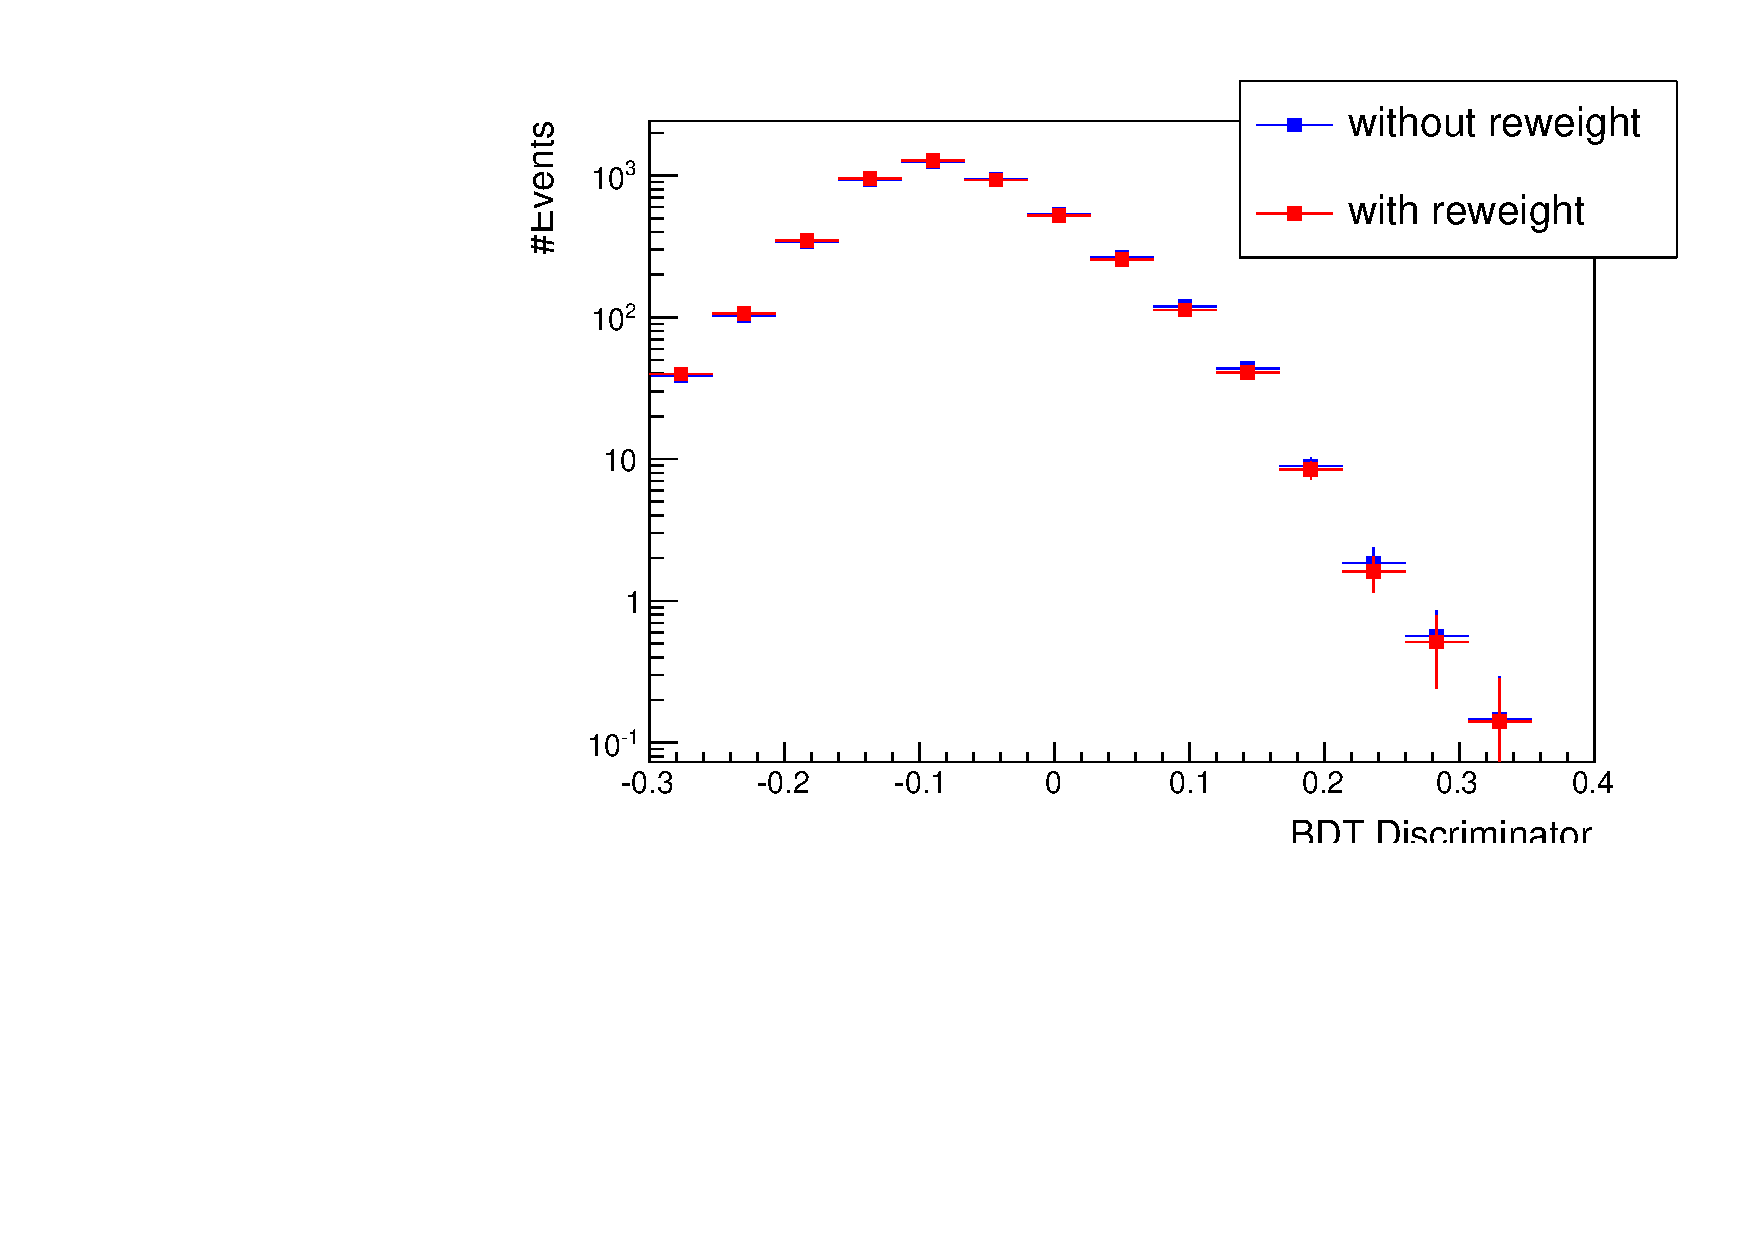
\includegraphics[width=0.49\textwidth]{images/Run1/ptrw_xcheck.pdf}
    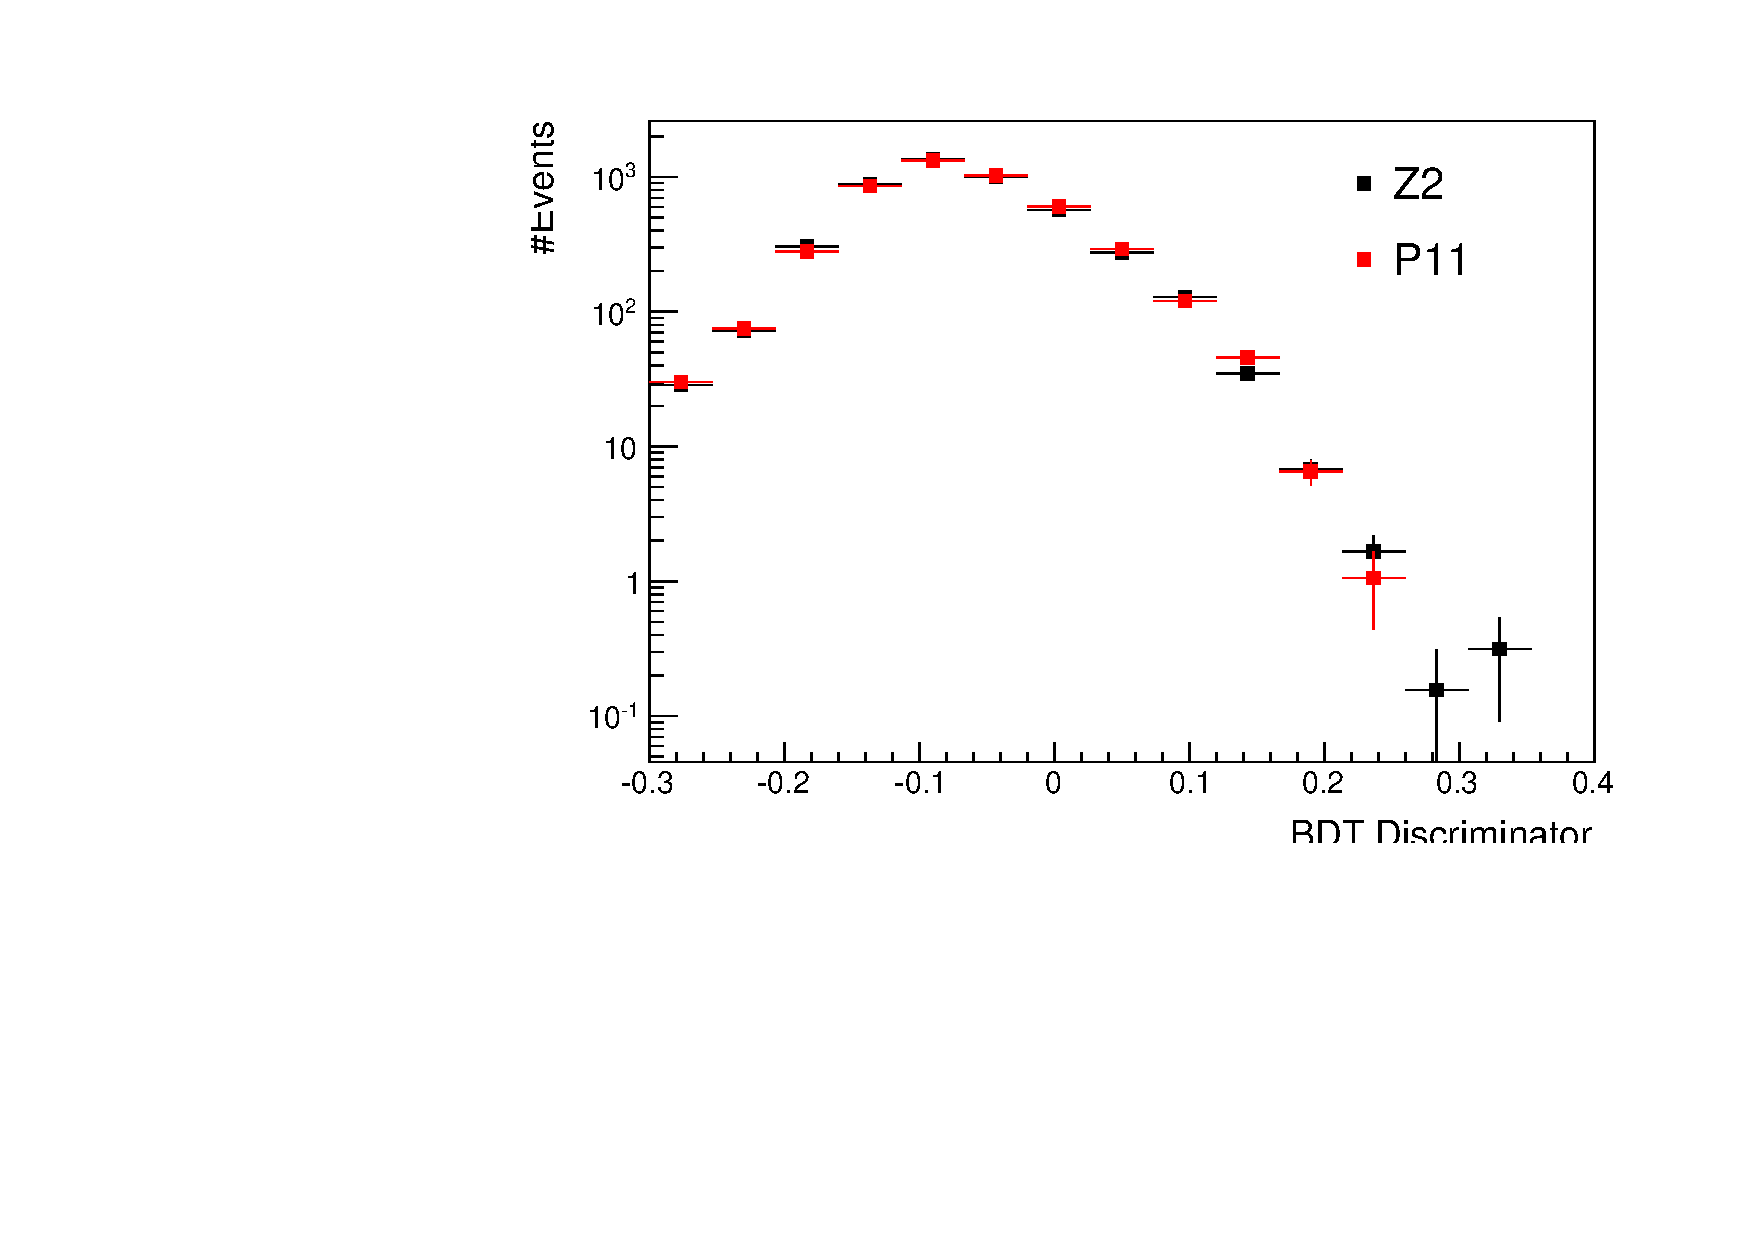
\includegraphics[width=0.49\textwidth]{images/Run1/NomTune_Mu_Log.pdf}\\
        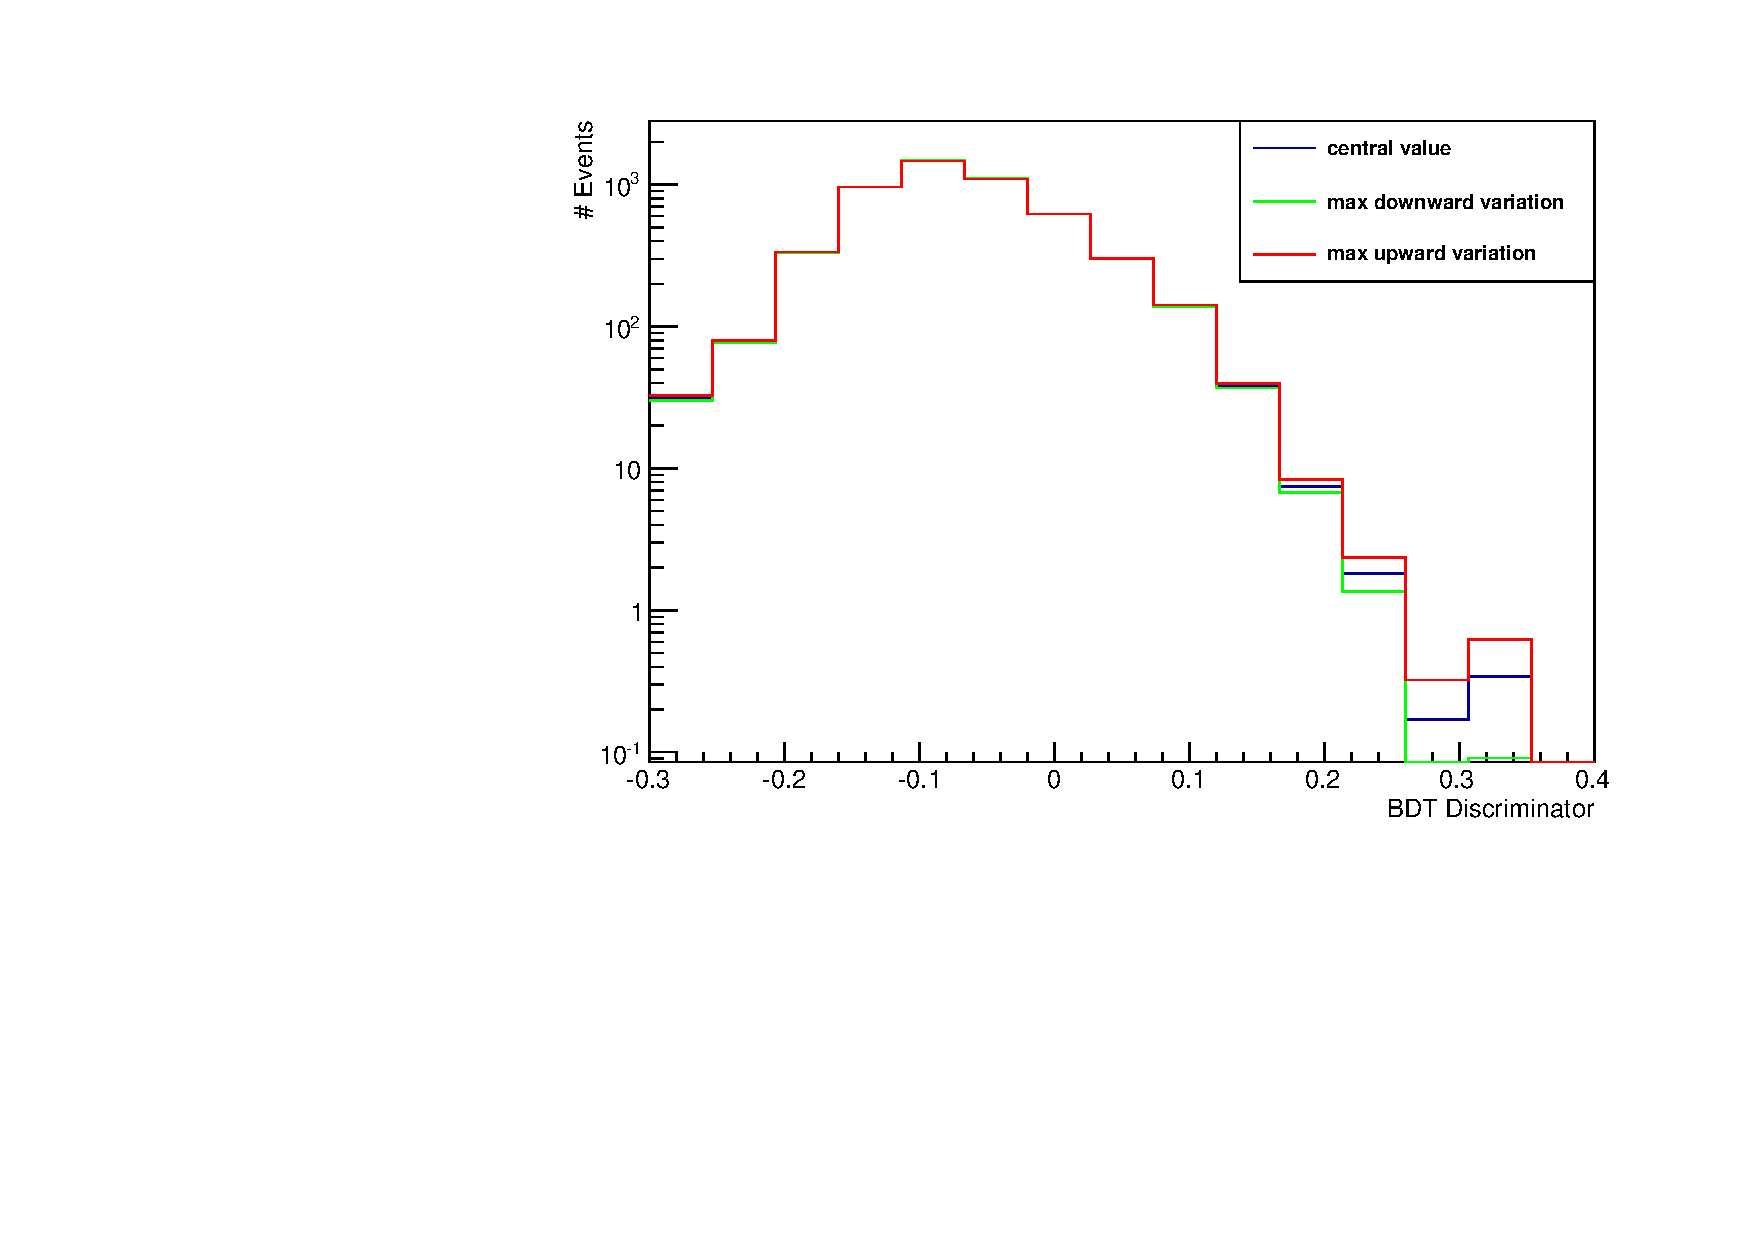
\includegraphics[width=0.7\textwidth]{images/Run1/PDF_uncertainty_mu.pdf}
    \caption{The BDT discriminator distributions of \ttbar simulation with and without the top quark \pt reweighting (top left), \PYTHIA tunes (top right) and PDF uncertainty (bottom)}
    \label{fig:studies8}
\end{figure}


\subsection{Individual effects of systematics}

To deduce how much of an effect each shape systematic has on the results, the expected limits were recalculated multiple times with one of the systematic effect removed. These limits are denoted lim.$_{1}$. In addition, another set of limits are calculated with only one of the systematic uncertainties included. These limits are denoted lim.$_{1}$. The values of lim.$_{1}$ and lim.$_{2}$ for each systematic uncertainty are detailed in Table~\ref{tab:effectLims}.

\begin{table}[ht!]
\small
\centering
\begin{tabular}{|c |c |c | c | c | c |}
\hline
 Sys. &  exp. lim.$_{1}$ & exp. lim.$_{2}$   \\
 \hline   
 JER &    $33.15^{+13.84}_{-10.35}$  &  $30.19^{+14.21}_{-9.66}$    \\
 \hline  
 JES  & $31.62^{+15.05}_{-9.16}$ &  $23.31^{+12.25}_{-8.05}$     \\
\hline  
Matching &  $32.79^{+14.37}_{-10.21}$ & $32.79^{+14.37}_{-10.21}$     \\  
 \hline  
 PU    &  $32.42^{+13.91}_{-10.00}$  &  $28.05^{+13.32}_{-8.93}$    \\
 \hline  
 Scale  &  $32.46^{+14.56}_{-10.35}$ & $24.80^{+13.21}_{-6.73}$       \\
 \hline  
 bTag &  $33.40^{+14.27}_{-10.48}$ & $23.32^{+12.71}_{-8.35}$       \\
 \hline  
 leptonSF &  $33.36^{+14.24}_{-10.39}$  &  $28.20^{+13.32}_{-8.96}$   \\  
 \hline  
 misTag &  $33.24^{+14.14}_{-10.34}$  &  $28.62^{+13.46}_{-9.13}$  \\
 \hline  
 ttbb  &  $33.23^{+13.87}_{-10.17}$  &  $27.97^{+13.26}_{-8.91}$  \\
 \hline
\end{tabular}
\caption{Effects of systematic uncertainties. }
\label{tab:effectLims}
\end{table}

\subsection{Cross checks with Theta package and the fully-frequentist approach using Combine}

A cross-check is performed using the Theta package~\cite{theta} to set a limit using \CLS with the asymptotic approximation. As another cross-check, the fully frequentist \CLS limit setting procedure is performed, using Combine, in place of the asymptotic limit setting used for the final results. Due to the extremely large CPU demands of the fully frequentist technique the range of values for the parameter of interest, $\frac{\sigma_{tttt}}{\sigma_{tttt}^{SM}}$, and the number of points investigated is reduced. The results, shown in Table~\ref{tab:ThetaFreq}, are consistent with the results obtained using the asymptotic approximation in Combine.


\begin{table}[ht!]
\centering
\begin{tabular}{|l|r|r|r|r|}
 \hline 
 Setup & Exp.$\frac{\sigma_{signal}}{\sigma_{SM}^{t\bar{t}t\bar{t}}}$ & Obs.$\frac{\sigma_{signal}}{\sigma_{SM}^{t\bar{t}t\bar{t}}}$ & Exp.(fb) &Obs.(fb) \\ 
\hline
{\color{blue}Combine (asymptotic.)} & {\color{blue} 24.6 $\pm$ 13}  & {\color{blue}24.7} & {\color{blue} 32  $\pm$ 17}  & {\color{blue}32} \\
\hline
%Theta (asymptotic) & 21.9^{+10}_{-6} & 22.33 & 28.47^{+13}_{-8} & 29.02 \\
Theta (asymptotic) & $27.4^{+12}_{-8}$ & 24.66 & $35.6^{+16}_{-10}$ & 32 \\
 \hline
%Combine (ful. freq.) &  -  & 20.52 &  -  & 26.68 \\
Combine (ful. freq.) &  -  & 23.78 &  -  & 31 \\
\hline
\end{tabular}
\caption{CL$_S$ limits on $\sigma_{t\bar{t}t\bar{t}}$ from combine (asymptotic + fully frequentist) and Theta approaches.}
\label{tab:ThetaFreq}
\end{table}


\subsection{Fitted nuisance parameters and uncertainties}

% As previously described in Section~\ref{sec:limitsJS}, the four largest shape uncertainties (Scale, Matching, JES and B-tag scale factor) are constrained in the fit using gaussian terms with exponential interpolation. The nuisance parameters associated to the other shape systematics are constrained in the fit using gaussian terms and the nuisance parameters associated to the normalisation uncertainties are constrained in the fit using lognormal terms. 

In Table~\ref{tab:nuisBSB} the fitted values, $\Delta x$, and the post-fit uncertainties, $\sigma_{\text{out}}$, in units of the input uncertainty, $\sigma_{\text{in}}$, are given for the background only (b-only) hypothesis and the signal + background (s+b) hypothesis. If the associated uncertainty is well modelled, the value of $\frac{\Delta x}{\sigma_{\text{in}}}$ should be close to zero and the value of $\frac{\sigma_{\text{out}}}{\sigma_{\text{in}}}$ should be close to one. The largest deviations in $\frac{\sigma_{\text{out}}}{\sigma_{\text{in}}}$ arise from the scale and matching uncertainties, which is expected as these uncertainties were assigned ad hoc variations. Table~\ref{tab:nuisBSB} shows that the results do not vary significantly between the b-only and s+b hypothesises which is consistent with no signal being present in the data.

\begin{table}[ht!]
\centering
\begin{tabular}{|l|r|r|r|r|} \hline 
&  \multicolumn{2}{c|}{$b$-only fit } & \multicolumn{2}{c|}{$s+b$ fit} \\ 
name  &  $\Delta x/\sigma_{\text{in}}$ & $\sigma_{\text{out}}/\sigma_{\text{in}}$ & $\Delta x/\sigma_{\text{in}}$ &$\sigma_{\text{out}}/\sigma_{\text{in}}$  \\  \hline
btag                        &   +0.16 &  1.15 &   +0.16 & 1.24  \\
ew\_norm               &    -0.01 &  0.99 &   -0.00  & 0.99  \\
JEE                           &    +0.64 &  0.48 &  +0.63 & 0.49  \\
JES                          &    +0.30 &  0.37 &  +0.29  & 0.37  \\
lepton sf                  &    -0.02  &  1.19 &  -0.02  & 1.29  \\
lumi                        &    -0.92  &  0.81 &  -0.93  & 0.82  \\
matching                &    -0.30  &  0.17 &   -0.30 & 0.17  \\
mistag                    &    +0.22  & 1.04 &  +0.27 & 1.05  \\
pu                           &    +0.27 &  0.82 &  +0.28 & 0.86  \\
scale                      &     +0.12 &  0.25 &  +0.11 & 0.27  \\
tt\_norm                 &     -1.34  &  0.61 &  -1.35  & 0.62 \\
ttbb                        &      +0.18 &  0.84 & +0.20 & 0.87  \\
ttother\_norm         &     -0.06   & 0.99 &  -0.06 & 0.99  \\
\hline
\end{tabular}
\caption{Fitted values and post-fit uncertainties in units of input uncertainties ($\sigma_{in}$) for nuisance parameters in $b$-only and $s+b$ fits.}
\label{tab:nuisBSB}
\end{table}

% \subsection{Goodness-of-fit test}

% A goodness-of-fit test for a maximum likelihood fit based on a saturated model \cite{ref:CousinsSat} is also performed. A likelihood ratio ($\lambda$) is calculated in which the numerator is the value of the maximised likelihood function in the fit and the denominator is the maximum value of a likelihood function of a \emph{saturated model} i.e., a model that fits the data exactly. The quantity $-2 ln(\lambda)$ asymptotically follows a $\chi^{2}$ distribution and hence can be used as a test of the goodness of fit. Distributions are shown  for the background only hypothesis and the signal+background hypothesis in Fig. \ref{fig:GOF}. The corresponding p-value obtained for the fit using the method just described are provided below and indicate a good fit.

% \begin{centering}
% \begin{equation*}
% \centering
% p-value^{b-only} = 0.65 , \;\;\;\; p-value^{s+b} = 0.64 
% \end{equation*}
% \end{centering}

% \begin{figure}[ht!]
% \centering
%     \includegraphics[width=0.49\textwidth]{goodnessoffit_bonly.pdf}
%      \includegraphics[width=0.49\textwidth]{goodnessoffit_floatingsignal.pdf}
%     \caption{$\lambda$ test-statistic distributions in the b-only(left) and s+b hypotheses(right). }
%     \label{fig:GOF}
% \end{figure}

% \clearpage

\subsection{Alternative parameterisations}

%\subsection{Scale uncertainty}
As the scale systematic may vary in shape across the \njets categories, another cross-check on the analysis was to allow the scale systematic to vary independently in each \njets category, as in ~\cite{ref:heavyquarksSplit, ref:B2G-12-004}. In this approach, both channels have three nuisance parameters for the scale systematic compared with one nuisance parameter used for all \njets categories. The results, shown in Table~\ref{tab:limsScale}, show no significant change in the limit compared with the original approach. The associated nuisance parameters and their uncertainties are show in Table~\ref{tab:ScaleParamUnc}.

\begin{table}[ht!]
\centering
\begin{tabular}{| l | l | l | p{1cm} |}
 \hline 
$N_{scale \; params.}$ & Exp. (fb) &Obs. (fb) \\
\hline
%1 & 26.3\pm{13}$ & 27 \\
1&{\color{blue} 32  $\pm$ 17}  & {\color{blue}32}\\
 \hline
3  &  $31.8\pm{12}$ & 32.5 \\
\hline
\end{tabular}
\caption{CLS limits on $\sigma_{t\bar{t}t\bar{t}}$ for the nominal result (top row) and with scale uncertainty fit independently in each \njets bin (bottom row). }
\label{tab:limsScale}
\end{table}

\begin{table}[ht!]
\centering
\small
\begin{tabular}{|l|r|r|r|r|} \hline 
 &  \multicolumn{2}{c|}{$b$-only fit } & \multicolumn{2}{c|}{$s+b$ fit} \\
name        &  $\Delta x/\sigma_{\text{in}}$ & $\sigma_{\text{out}}/\sigma_{\text{in}}$ & $\Delta x/\sigma_{\text{in}}$ &$\sigma_{\text{out}}/\sigma_{\text{in}}$  \\  \hline
btag          &    +0.04& 1.35 & -0.04& 1.51 \\
jer             &      +0.43& 0.53 &     +0.42& 0.54 \\
jes            &   +0.30& 0.37 &  +0.28& 0.39  \\
leptonsf    &      -0.01& 1.36 &  -0.02& 1.56 \\
lumi          &      -0.92& 0.81 &     -0.94& 0.82  \\
matching  &   -0.27& 0.19 &  -0.26& 0.19  \\
mistag      &      +0.18& 1.17 &     +0.27& 1.13  \\
pu            &      +0.29& 0.87 &     +0.28& 0.95  \\
scale6j     &   +0.31& 0.23 &  +0.31& 0.23  \\
scale7j     &   +0.31& 0.25 &  +0.31& 0.25  \\
scale8j     &   -0.71& 0.34 &  -0.70& 0.36  \\
tt\_norm   &      -1.33& 0.61 &     -1.36& 0.62  \\
ttbb          &      +0.40& 0.71 &     +0.44& 0.75  \\
 \hline
\end{tabular}
\vspace{-0.2cm}
\caption{Fitted values and post-fit uncertainties in units of input uncertainties ($\sigma_{in}$) for all nuisance parameters in $b$-only and $s+b$ fits.}
\label{tab:ScaleParamUnc}
\end{table}

A separate check was made where the normalisation uncertainty on the $\ttbar$ component was allowed to vary independently in each  \njets category. In each channel, three nuisance parameters are associated to the normalisation uncertainty on the $\ttbar$ for each \njets category compared to the one nuisance parameter across all \njets categories in the original approach. The results, shown in Table~\ref{tab:limsTTnorm}, also show no significant change to the original limit.

%\subsection{t\bar{t}$ normalisation uncertainty}

\begin{table}[ht!]

\centering
\begin{tabular}{| l | l | l | p{1cm} |}
 \hline 
& Exp. (fb) &Obs. (fb) \\
\hline
%1 & 26.3\pm{13}$ & 27 \\
nominal&{\color{blue} 32  $\pm$ 17}  & {\color{blue}32}\\
 \hline
varying tt in \njets bins  &  36 $\pm {17}$ & 41 \\
\hline
\end{tabular}
\caption{CLS limits on $\sigma_{t\bar{t}t\bar{t}}$ for the nominal result (top row) and with tt normalisation uncertainty fit independently in each \njets bin (bottom row). }
\label{tab:limsTTnorm}
\end{table}


\subsection{Using \njets$\geq$8jet category only}

The greatest separation of signal and background occurs in the \njets$\geq$8jet category as $\tttt$ events are typically higher jet multiplicity events than $\ttbar$. In order to ascertain whether the analysis could benefit from a higher jet multiplicity cut, the limit setting procedure is repeated using only the \njets$\geq$8jet category . The results are shown in Table \ref{tab:lims8}, where it can be seen that the limit is made worse by removing the \njets$=6$ and \njets$=7$ categories. This confirms that including the \njets$=6$ category aids in constraining the $\ttbar$ in the fit. The \njets$=7$ category also has some discrimination between signal and background and simultaneously fitting the \njets$=6$, \njets$=7$ and \njets$\geq8$ categories provides a better limit.

\begin{table}[ht!]
\centering
\begin{tabular}{| l | l | l | p{1cm} |}
 \hline 
  & Exp. (fb) &Obs. (fb) \\
\hline
%nominal result & 26.3\pm{13}$ & 27 \\
 {\color{blue} nominal result}&{\color{blue} 32  $\pm$ 17}  & {\color{blue}32}\\
 \hline
8 jet bin only  &  $45 \pm{ 17}$  & 47 \\
\hline
\end{tabular}
\caption{CLS limits on $\sigma_{t\bar{t}t\bar{t}}$ for nominal scenario and 8 jet bin only. }
\label{tab:lims8}
\end{table}

\subsection{Investigation of binning in BDT distributions \label{appsub:binning}}

In order to ascertain what the optimum binning should be within each BDT distribution, a variety a values are plotted in Fig.~\ref{fig:Binning}. Both the inclusive result before splitting the templates into \njets categories and exclusive \njets categories results are shown, where the significant improvement in the limit by the latter method can be seen. The limit does not appear the improve significantly by increasing the number of bins in the BDT distributions so in order to ensure that most bins were well populated, the number of bins was chosen to be ten in the exclusive analysis.

\begin{figure}[ht!]
\centering
    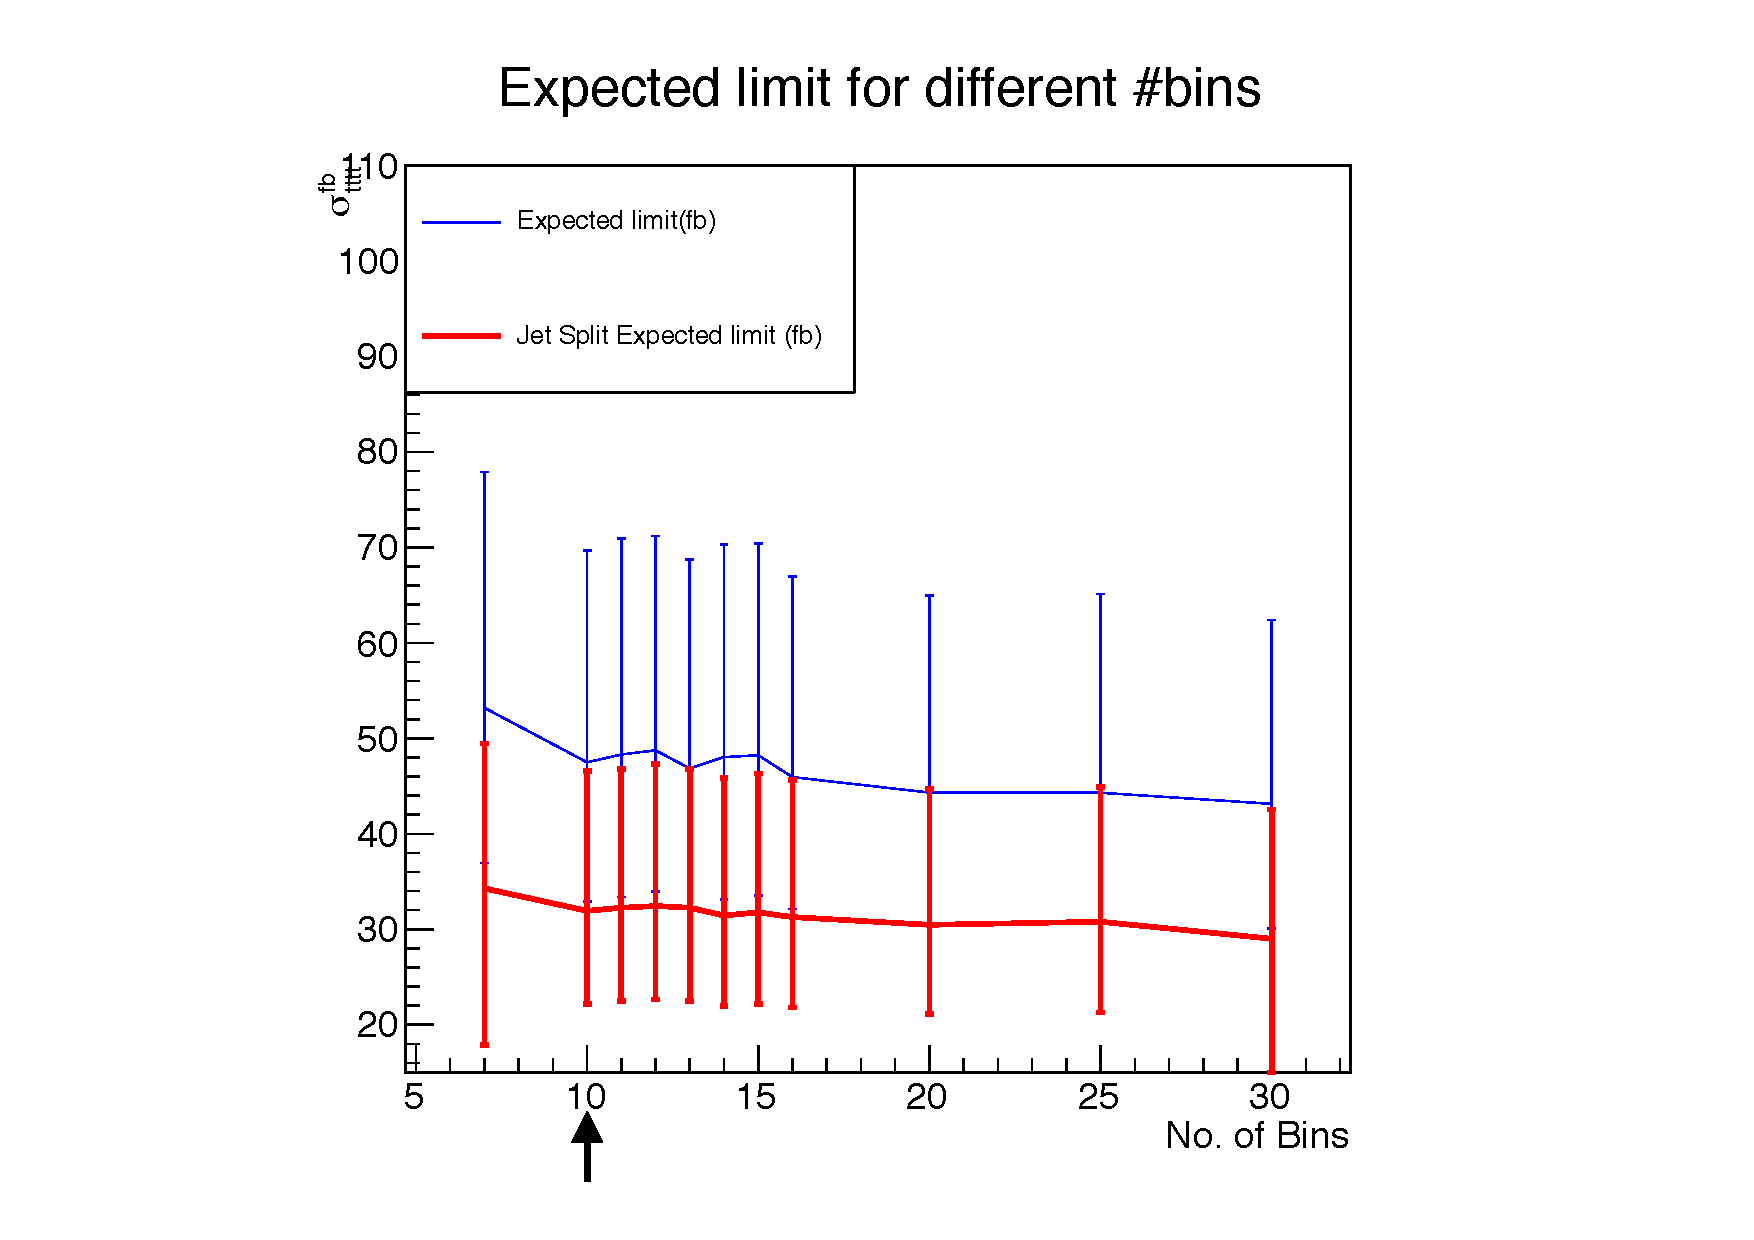
\includegraphics[width=0.69\textwidth]{images/Run1/BinningPrint.pdf}
    \caption{Fitted values(fb) and observed(fb) for various injected signal strength(fb).}
    \label{fig:Binning}
\end{figure}

\section{Summary and conclusion}
\label{sec:summary8}
The full 2012 data set of proton-proton collisions at $\sqrt{s}=8$~TeV with 19.7~\fbinv of data was used to set limits on the production of \tttt in the single muon and single electron final states in the absence of a signal. After a baseline selection the dominant background is \ttbar production. The simulation is corrected with scale factors. Two BDTs are used in the analysis, one for reconstructing hadronically decaying top quarks and one event-level BDT to separate the signal and background using discriminators derived from the hadronic top quark reconstruction BDT. Analysis of the systematic uncertainties showed the factorisation and renormalisation scale on the \ttbar background to be the largest uncertainty. A template fit was performed on the templates of the event-level BDT discriminator output which was separated into \njets categories. A simulataneous fit of the templates for the single electron and single muon histograms, each split into \njets categories, was performed and a \CLS limit on $\sigmatttt~/~\sigmattttSM$ of 25 observed and $24.6\pm13$ expected was found. This corresponds to 32~\fb observed with $32.0\pm17$~\fb expected.

\section{Discussion of ATLAS four-top-quark production studies at $\sqrt{s} =$~8~TeV}
\label{sec:ATLASresult}
% \fxnote{Possible comparison with atlas requirements put into our framework}

\section{MANY TABLES FROM AN}

\fxnote*{?}{These were performed by James so not sure whether to include. Maybe they have useful information}


\begin{table}[ht!]
\centering
\begin{tabular}{|c lc |c |c l p{1cm} |}
 \hline 
Parameter &   Value & $\sigma_{parabolic}$  \\
  \hline   
 $\frac{\sigma_{\tttt}}{\sigma^{SM}_{\tttt}}$  & 0.0034   & 65.7 \\
  \hline  
 Lumi    &     0.96 &  0.03   \\
   \hline  
  $\alpha_{JER}$ &   0.7 &  0.07  \\ 
  \hline  
  $\beta_{JES}$  & 1.00   & 0.01    \\
  \hline  
  $\beta_{Matching}$ & 0.999 &  0.0062\\  
  \hline  
  $\alpha_{PU}$    & 0.41  & 0.79 \\
  \hline  
  $\beta_{Scale}$  & 1.00 & 0.006  \\ 
  \hline  
  $\beta_{bTag}$ & 1.00  & 0.007  \\
  \hline  
  $\alpha_{leptonSF}$ & 0.00031 & 0.17 \\   
  \hline  
  $\alpha_{misTag}$ & -0.00005  & 0.19 \\
  \hline  
  $\alpha_{ttbb}$  & -0.32  & 0.12  \\
  \hline
\end{tabular}
\begin{tabular}{|c lc |c |c l p{1cm} |}
 \hline 
 Parameter &   Value & $\sigma_{parabolic}$  \\
  \hline   
 $\frac{\sigma_{\tttt}}{\sigma^{SM}_{\tttt}}$  & 21.7  & 23.4  \\
  \hline  
  Lumi    &     0.98 &  0.028   \\
  \hline  
  $\alpha_{JER}$ &   -0.0083 &  0.53  \\ 
  \hline  
  $\beta_{JES}$  & 0.92   & 0.056   \\
  \hline  
  $\beta_{Matching}$ & 0.99 &  0.005   \\  
  \hline  
  $\alpha_{PU}$    & -0.00012  & 0.15  \\
  \hline  
  $\beta_{Scale}$  & 1.00 & 0.01   \\ 
  \hline  
  $\beta_{bTag}$ & 0.99     & 0.03   \\
  \hline  
  $\alpha_{leptonSF}$ & 0.3 &0.91  \\   
  \hline  
  $\alpha_{misTag}$ & 0.26  & 0.89  \\
  \hline  
  $\alpha_{ttbb}$  & 0.38  & 0.86   \\
  \hline
\end{tabular}
\caption{The fitted values and errors of the parameters resulting from fits to the BDT discriminator distributions for the $\mu$ + jets channel (left) and $e$ + jets channel (right). Lognormal pdfs are used to model the source of large systematic uncertainty (Scale, Matching, JES, B-tag). Truncated gaussian pdfs are used to model the other sources of systematic uncertainty. }
\label{tab:fittedparams1}
\end{table}



\begin{table}[ht!]
\centering
\begin{tabular}{| c c cc c |}
\hline  
%Parameter &   Value & Parabolic Error (approx.) & MINOS errors \\
  Parameter &   Value & $\sigma_{parabolic}$ &    $\frac{Value-Nominal}{\sigma_{parabolic}}$ &    $\frac{Value-Nominal}{\sigma_{prior}}$ \\
\hline   
$\frac{\sigma_{\tttt}}{\sigma^{SM}_{\tttt}}$  & 14.2  & 20.5 & 0.695 & - \\
    \hline  
    Lumi  &   0.98 &  0.022  & 0.91 & 0.77 \\
    \hline  
    $\alpha_{JER}$ &   0.26 &  0.62   & 0.42 & 0.26 \\  
    \hline  
    $\beta_{JES}$  & 0.97  & 0.05   & 0.6  &  0.3  \\
    \hline   
    $\beta_{Matching}$ & 0.99 &  0.005   & 2  & 0.5 \\  
    \hline  
    $\alpha_{PU}$  & 0.012  & 0.67 &  0.02 & 0.012 \\
    \hline  
    $\beta_{Scale}$  & 1.0001  & 0.0433   & 0.002  & 0.0005 \\ 
    \hline  
    $\beta_{bTag}$ & 0.99    & 0.027   & 0.37   &  0.25 \\
    \hline  
    $\alpha_{leptonSF}$ & 0.23 & 0.85    & 0.27    &  0.23 \\   
    \hline  
    $\alpha_{misTag}$ & 0.095   & 0.817   & 0.12  & 0.095 \\
    \hline  
    $\alpha_{ttbb}$  & 0.55  & 0.74 & 0.74  & 0.55\\
    \hline
\end{tabular}
\caption{Combined: The fitted values and errors of the parameters resulting from the combined fit to the BDT discriminator distributions. Lognormal pdfs are used to model the source of large systematic uncertainty (Scale, Matching, JES, B-tag). Truncated gaussian pdfs are used to model the other sources of systematic uncertainty. }
\label{tab:fittedparams2}
\end{table}

\begin{table}[ht!]
\centering
\begin{tabular}{| c c cc c |}
 \hline  
    Parameter &   Value & $\sigma_{parabolic}$ &    $\frac{Value-Nominal}{\sigma_{parabolic}}$ &    $\frac{Value-Nominal}{\sigma_{prior}}$ \\
    \hline   
    $\alpha_{\ttbar}$ &   -1.08 &  0.64 &  -1.69 & -1.08 \\  
    \hline  
    $\alpha_{\ttbar other}$  & -0.11  & 0.99 & -.11  & -0.11  \\
    \hline   
    $\alpha_{EW}$ & -0.073 &  0.99 &  -0.073 & -0.073  \\  
    \hline  
\end{tabular}
\caption{Combined: The fitted values and errors of the parameters resulting describing the normalisation uncertainties of the background components from the combined fit to the BDT discriminator distributions. Truncated gaussian pdfs are used to model these uncertainties. }
\label{tab:fittedparams3}
\end{table}


\begin{table}[ht!]
\centering
\begin{tabular}{| c c cc c |}
\hline  
  Parameter &   Value & $\sigma_{parabolic}$ &    $\frac{Value-Nominal}{\sigma_{parabolic}}$ &    $\frac{Value-Nominal}{\sigma_{prior}}$ \\
\hline   
$\frac{\sigma_{\tttt}}{\sigma^{SM}_{\tttt}}$  & 1.09  & 0.19 & 0.47 & - \\
    \hline  
    Lumi  &   0.98 &  0.022  & 0.91 & 0.77 \\
    \hline  
    $\alpha_{JER}$ &   0.16 &  0.76   & 0.21 & 0.16 \\  
    \hline  
    $\beta_{JES}$  & 0.96  & 0.05   & 0.8  &  0.4  \\
    \hline   
    $\beta_{Matching}$ & 0.99 &  0.004   & 2.5  & 0.5 \\  
    \hline  
    $\alpha_{PU}$  & 0.047  & 0.7 &  0.07 & 0.047 \\
    \hline  
    $\beta_{Scale}$  & 1.00007  & 0.01   & 0.007  & 0.0004 \\ 
    \hline  
    $\beta_{bTag}$ & 0.99    & 0.23   & 0.04   &  0.25 \\
    \hline  
    $\alpha_{leptonSF}$ & 0.15 & 7.4    & 0.002    &  0.15 \\   
    \hline  
    $\alpha_{misTag}$ & -0.005   & 0.78   & 0.0064  & -0.005 \\
    \hline  
    $\alpha_{ttbb}$  & 0.48  & 1.2 & 0.38  & 0.48\\
    \hline
\end{tabular}
\caption{Combined: The fitted values and errors of the parameters resulting from the combined fit to the BDT discriminator distributions in the null hypothesis.}
\label{tab:fittedparams4}
\end{table}

\begin{table}[ht!]
\centering
\begin{tabular}{| c c cc c |}
 \hline  
    Parameter &   Value & $\sigma_{parabolic}$ &    $\frac{Value-Nominal}{\sigma_{parabolic}}$ &    $\frac{Value-Nominal}{\sigma_{prior}}$ \\
    \hline   
    $\alpha_{\ttbar}$ &   -1.02 &  0.62 &  -1.69 & -1.02 \\  
    \hline  
    $\alpha_{\ttbar other}$  & -0.1  & 0.99 & -0.11  & -0.1  \\
    \hline   
    $\alpha_{EW}$ & -0.07 &  0.99 &  -0.073 & -0.07  \\  
    \hline  
\end{tabular}
\caption{Combined: The fitted values and errors of the parameters resulting describing the normalisation uncertainties of the background components from the combined fit to the BDT discriminator distributions in the null hypothesis. }
\label{tab:fittedparams5}
\end{table}



\begin{figure}[ht!]
    \includegraphics[width=0.49\textwidth]{images/Run1/FitParams_compare_lognorm.pdf}
      \includegraphics[width=0.49\textwidth]{images/Run1/FitParams_compare_truncgaus.pdf}
    \caption{The fitted values and approximate errors for the lognormal (left) and truncated gaussian (right) nuisance parameters describing the shape systematics.}
    \label{fig:comparefittedparams}
\end{figure}




\begin{table}[ht!]
\centering
\begin{tabular}{| c c cc c |}
\hline  
  Parameter &   Value & $\sigma_{parabolic}$ &    $\frac{Value-Nominal}{\sigma_{parabolic}}$ &    $\frac{Value-Nominal}{\sigma_{prior}}$ \\
\hline   
$\frac{\sigma_{\tttt}}{\sigma^{SM}_{\tttt}}$  & 0.4  & 21.3 &  0.03 & - \\
    \hline  
    Lumi  &   0.98 &  0.01  & 1.4 & 0.76  \\
    \hline  
    $\alpha_{linear}$ & -0.17 &  0.38   & -0.45  & -0.17  \\  
    \hline  
    $\alpha_{parabolic}$ & -0.25 &  0.28   & -0.9  & -0.25  \\  
    \hline  
    $\alpha_{JER}$ & 0.11 &  0.43   & 0.26  & 0.11  \\  
    \hline  
    $\beta_{JES}$  & 0.97  & 0.02   &  1.5 & 0.3   \\
    \hline   
    $\beta_{Matching}$ & 0.99 &  0.003   & 2.3   & 0.35 \\  
    \hline  
    $\alpha_{PU}$  & 0.016  & 0.43 & 0.04 &  0.016 \\
    \hline  
    $\beta_{Scale}$  & 0.9992 & 0.17   & 0.005  & 0.004 \\ 
    \hline  
    $\beta_{bTag}$ & 1.002    & 0.02   &  0.1  &  0.05 \\
    \hline  
    $\alpha_{leptonSF}$ & 0.05 & 0.45    &  0.11   & 0.05   \\   
    \hline  
    $\alpha_{misTag}$ & 0.071   & 0.48   & 0.15  &   0.071 \\
    \hline  
    $\alpha_{ttbb}$  & 0.34  & 0.44 &  0.77 & 0.34 \\
    \hline
\end{tabular}
\caption{Combined: The fitted values and errors of the parameters resulting from the combined fit to the BDT discriminator distributions with extra nuisance parameters ($\alpha_{linear}$ and $\alpha_{parabolic}$) included.  }
\label{tab:extraparams1}
\end{table}


\begin{table}[ht!]
\centering
\begin{tabular}{| c c cc c |}
 \hline  
    Parameter &   Value & $\sigma_{parabolic}$ &    $\frac{Value-Nominal}{\sigma_{parabolic}}$ &    $\frac{Value-Nominal}{\sigma_{prior}}$ \\
    \hline   
    $\alpha_{\ttbar}$ &   -1.04 &  0.42 & -2.47  & -1.04  \\  
    \hline  
    $\alpha_{\ttbar other}$  & -0.08  &0.73 & -0.11 & -0.08 \\
    \hline   
    $\alpha_{EW}$ & -0.07 &  0.75 &  -0.1 &  -0.07\\  
    \hline  
\end{tabular}
\caption{Combined: The fitted values and errors of the parameters resulting describing the normalisation uncertainties of the background components from the combined fit to the BDT discriminator distributions after the inclusion of extra nuisance parameters. }
\label{tab:extraparams2}
\end{table}




\begin{table}[ht!]
\small
\centering
\begin{tabular}{|c |c |c | c | c | c |}
 \hline 
Sys. &   \% $\Delta N_{events}$ (\ttbar) &  \% $\Delta N_{events}$ (\tttt)   \\
\hline  
Lumi &  4 &  4    \\
\hline  
JER &   $^{+3.7}_{-0.40}$ &  -    \\ 
\hline  
JES  & $^{+11}_{-12}$  & -   \\
\hline  
Matching &$^{+4}_{-6}$ &  -     \\  
\hline  
PU    & $\pm 1.5$   & -    \\
\hline  
Scale  & $^{+27}_{-20}$  & -     \\ 
\hline  
bTag &  $\pm 3.9 $    & -        \\
\hline  
leptonSF & $\pm .4 $& -    \\   
\hline  
misTag & $\pm 6.9 $    & - \\
\hline  
ttbb  & $\pm 1.4$  & - \\
\hline
\end{tabular}
\begin{tabular}{|c |c |c | c | c | c |}
 \hline 
Sys. &   \% $\Delta N_{events}$ (\ttbar) &  \% $\Delta N_{events}$ (\tttt)   \\
\hline  
Lumi &  $\pm 4$ &  $\pm 4$    \\
\hline  
JER &  $\pm 1.3$ &  $\pm 0.5$    \\ 
\hline  
JES  & $\pm 10$  & $\pm 2.1$    \\
\hline  
Matching &$^{+5}_{-2}$  &   -    \\  
\hline  
PU    & $\pm 0.4$  &   $\pm 0.2$   \\
\hline  
Scale  & $^{+31}_{-15}$  & -    \\ 
\hline  
bTag & $\pm 3.8$     &       $\pm 1.9$   \\
\hline  
leptonSF & $\pm 0.5$&  $\pm 0.5$  \\   
\hline  
misTag & $\pm 0.7$  &  $\pm 0.5$  \\
\hline  
ttbb  & $\pm 1.5$  & - \\
\hline
\end{tabular}
\caption{Effects of systematic uncertainties. }
\label{tab:yields}
\end{table}

